\chapter{薄板问题HR}
本章进一步介绍了带有挠度和弯矩双变量时薄板问题Hellinger-Reissner变分原理,随后通过对挠度采用再生核近似离散,弯矩在每个背景积分单元建立局部多项式离散的方式
构造了一种基于Hellinger-Reissner变分原理的变分一致性本质边界条件施加方法,最后通过数值算例进一步验证在高阶薄板问题时所提方法的变分一致性、计算精度和计算效率。
\section{Hellinger-Reissner变分原理}
Hellinger-Reissner变分原理不仅适用于解决弹性力学问题中的位移和应力之间的耦合现象,并且在结构力学中也广泛应用于薄板和壳体等问题的数值求解,
Hellinger-Reissner变分原理基于能量泛函的最小化原理,在薄板问题中引入了两个变分函数:挠度场的变分函数和弯矩场的变分函数。
通过构造能量泛函和变分操作,得到平衡方程和边界条件的弱形式,并通过数值方法求解离散化的方程组获得薄板的挠度和弯矩分布。
\par
基于Hellinger-Ressiner变分原理\cite{},四阶薄板问题控制方程式(\ref{P control equation})对应的余能泛函表达式为:
\begin{equation}\label{pfanhan}
\begin{split}
    \Pi_{H\!R}(M_{\alpha\beta},w)&=\int_{\Omega}\frac{1}{2}M_{\alpha\beta}C^{-1}_{\alpha\beta\gamma\eta}M_{\gamma\eta}d\Omega-\int_{\Gamma_w}V_{\pmb n}\bar{w}d\Gamma+\int_{\Gamma_{\theta}}M_{\pmb{nn}}\bar{\theta}_nd\Gamma-p\bar{w}\vert_{x\in{c_w}}\\
&+\int_{\Omega}w(M_{\alpha\beta,\alpha\beta}+\bar{q})d\Omega+\int_{\Gamma_M}w_{,\pmb n}(M_{\pmb{nn}}-\bar{M}_{\pmb{nn}})d\Gamma\\
&-\int_{\Gamma_V}w(V_{\pmb n}-\bar{V}_{\pmb n})d\Gamma-w(P-\bar{P})\vert_{x\in{c_P}}
\end{split}
\end{equation}\par
对余能泛函$\Pi_{H\!R}$进行变分得到式(\ref{P control equation})中带有挠度$w$和弯矩$M$双变量的伽辽金弱形式:
\newpage
\begin{equation}\label{Pweakfrom}
\begin{split}
    \delta\Pi_{H\!R}(M_{\alpha\beta,w})&=\int_{\Omega}\delta M_{\alpha\beta}D^{-1}_{\alpha\beta\gamma\eta}M_{\gamma\eta}d\Omega-\int_{\Gamma_w}\delta V_{\pmb n}\bar{w}d\Gamma+\int_{\Gamma_{\theta}}\delta M_{\pmb{nn}}\bar{\theta}_nd\Gamma-\delta P\bar{w}_{x\in{c_w}}\\
    &+\int_{\Omega}\delta M_{\alpha\beta,\alpha\beta}wd\Omega+\int_{\Gamma_M}\delta M_{\pmb{nn}}w_{,\pmb n}d\Gamma-\int_{\Gamma_V}\delta V_{\pmb n}wd\Gamma-\delta Pw\vert_{x\in{c_P}}\\
    &+\int_{\Omega}\delta w(M_{\alpha\beta,\alpha\beta}+\bar{q})d\Omega+\int_{\Gamma_M}\delta w_{,n}(M_{nn}-\bar{M}_{nn})d\Gamma\\
    &-\int_{\Gamma_V}\delta w(V_{\pmb n}-\bar{V}_{\pmb n})d\Gamma-\delta w(P-\bar{P})\vert_{x\in{c_P}}\\
    &=0
\end{split}
\end{equation}\par
对能量泛函$\Pi_{H\!R}$取极值时,要求对任意的$\delta w$、$\delta M_{\alpha\beta}$关于$\delta\Pi_{H\!R}$都要恒成立,此时利用几何关系式:
\begin{equation}
    \begin{split}
    \Gamma=\Gamma_w\cup\Gamma_V\cup\Gamma_{\theta}\cup\Gamma_M,c=c_w\cup c_P\\
    \Gamma_w\cap\Gamma_V=\Gamma_{\theta}\cap\Gamma_M=c_w\cap c_P=\varnothing
\end{split}
\end{equation}
进一步将弱形式(\ref{Pweakfrom})根据$\delta w$、$\delta M_{\alpha\beta}$改写为下列两式:
\begin{equation}\label{Pweakform1}
    \begin{split}
        \int_\Omega {\delta {M_{\alpha \beta }}D_{\alpha \beta \gamma \eta }^{ - 1}{M_{\gamma \eta }}d\Omega }&=\int_\Gamma  {\delta {V_{\bf{n}}}wd\Gamma }  - \int_\Gamma  {\delta {M_{{\bf{nn}}}}{w_{,{\bf{n}}}}d\Gamma }+{\left. {\delta Pw} \right|_{{\bf{x}} \in c}} - \int_\Omega  {\delta {M_{\alpha \beta ,\alpha \beta }}wd\Omega } \\
        &-\int_{{\Gamma _w}} {\delta {V_{\bf{n}}}wd\Gamma }  + \int_{{\Gamma _\theta }} {\delta {M_{{\bf{nn}}}}{w_{,{\bf{n}}}}d\Gamma }  - {\left. {\delta Pw} \right|_{{\bf{x}} \in {c_w}}}\\
        &+\int_{{\Gamma _w}} {\delta {V_{\bf{n}}}\bar wd\Gamma }  - \int_{{\Gamma _\theta }} {\delta {M_{{\bf{nn}}}}{{\bar \theta }_{\bf{n}}}d\Gamma }  + {\left. {\delta P\bar w} \right|_{{\bf{x}} \in {c_w}}}
    \end{split}
\end{equation}
\begin{equation}
        \begin{split}\label{Pweakform2}
            &\int_\Gamma  {\delta w{V_{\bf{n}}}d\Gamma } - \int_\Gamma  {\delta {w_{,{\bf{n}}}}{M_{{\bf{nn}}}}d\Gamma }  + {\left. {\delta wP} \right|_{{\bf{x}} \in c}} - \int_\Omega  {\delta w{M_{\alpha \beta ,\alpha\beta}}d\Omega }\\
            &- \int_{{\Gamma _w}} {\delta w{V_{\bf{n}}}d\Gamma }  + \int_{{\Gamma _\theta }} {\delta {w_{,{\bf{n}}}}{M_{{\bf{nn}}}}d\Gamma }  - {\left. {\delta wP} \right|_{{\bf{x}} \in {c_w}}}\\
            &= \int_{{\Gamma _V}} {\delta w{{\bar V}_{\bf{n}}}d\Gamma }  - \int_{{\Gamma _M}} {\delta {w_{,{\bf{n}}}}{{\bar M}_{{\bf{nn}}}}d\Gamma }  + {\left. {\delta w\bar P} \right|_{{\bf{x}} \in {c_P}}} + \int_\Omega  {\delta w\bar qd\Omega} 
    \end{split}
\end{equation} 
\section{挠度-弯矩混合离散}
薄板挠度$w$采用基于再生核近似的无网格形函数进行离散。无网格法通过如图(\ref{PPSI})所示在薄板中面$\Omega$和边界$\Gamma$上布置一系列无网格节点$\{\pmb{x}_I\}^{N\!P}_{I=1}$进行离散,
不失为一般性,考虑任意薄板挠度$w$的近似表达式$w^h$及其虚位移$\delta w^h$可表示为:
\begin{equation}\label{w}
\begin{split}
    w^h(\pmb{x})=\sum_{I=1}^{N\!P}\Psi_I(\pmb{x})d_{I},\delta w^h(\pmb{x})=\sum_{I=1}^{N\!P}\Psi_I(\pmb{x})\delta d_I
\end{split}
\end{equation}
其中$N\!P$表示无网格节点数量,$d_I$、$\Psi_I(\pmb{x})$为无网格节点$\pmb{x}_I$上的节点系数和无网格形函数。
根据再生核近似理论\cite{}以及满足多项式一致性条件,无网格形函数的表达式为:
\begin{equation}
\begin{split}
    \Psi_I(\pmb{x})=\pmb{p}^T(\pmb{0})\pmb{A}^{-1}(\pmb{x})\pmb{p}(\pmb{x}_I-\pmb{x})\phi_s(\pmb{x}_I-\pmb{x})
\end{split}
\end{equation}
其中$\pmb{p}$为$p$阶的多项式基函数向量,$\pmb{A}$为矩量矩阵,核函数$\phi_s(\pmb{x}_I-\pmb{x})$选取五次样条函数。具体求解过程见第一章。\par
% \begin{figure}[H]
%     \centering
%     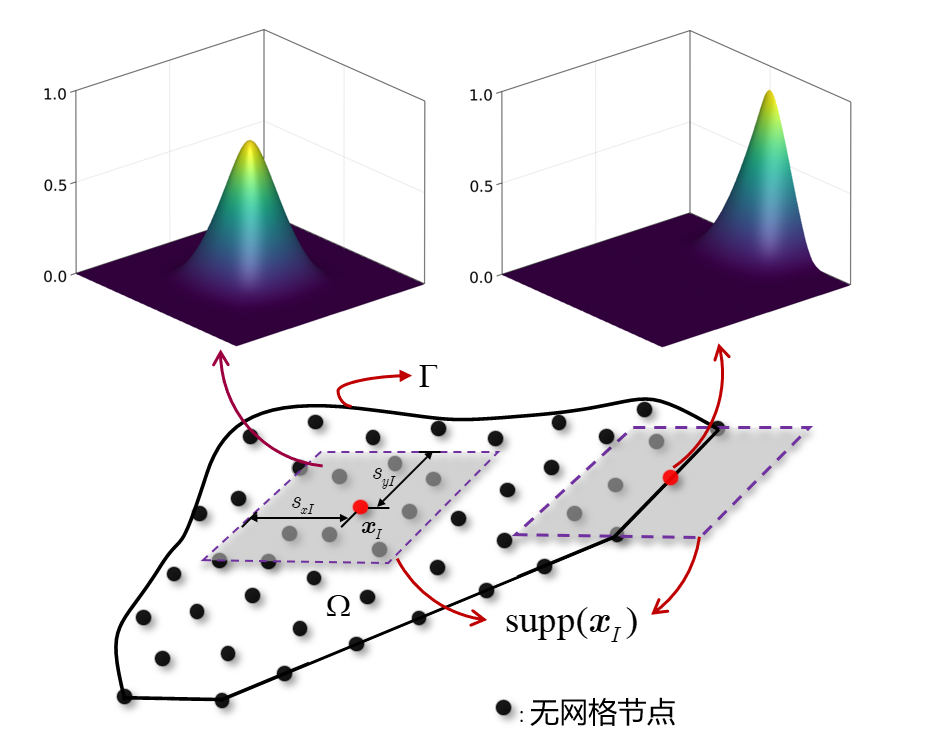
\includegraphics[scale=0.6]{figure/PHR/PSI.png}
%     \caption{薄板无网格离散}\label{PPSI}
% \end{figure}
弯矩分量$M_{\alpha\beta}$在每个背景积分单元建立局部的多项式进行离散。
如图(\ref{Pintegralscheme})所示,将薄板中面$\Omega$划分为一系列背景积分单元$\Omega_C,C=1,2,\dotsb,n_C$,并且存在$\cup_{C=1}^{N\!C}\Omega_C\thickapprox\Omega$。
在背景积分单元$\Omega_C$内,假定弯矩分量$M_{\alpha\beta}$以任意的多项式进行离散,并将离散后的弯矩分量$M_{\alpha\beta}$记为$M_{\alpha\beta}^h$
\begin{equation}\label{moment}
\begin{split}
    M^h_{\alpha\beta}(\pmb{x})=\pmb{a}_{\alpha\beta}^T\tilde{\pmb{q}}(\pmb{x})
\end{split}
\end{equation}
$\tilde{\pmb{q}}(\pmb{x})$是比多阶基函数向量$\pmb{p}(\pmb{x})$低两阶的单项式向量,具体表达式为:
\begin{equation}
\begin{split}
    \tilde{\pmb{q}}(\pmb{x})=\{1,\;x,\;y,\;\dots,\;x^iy^j,\;\dots,\;y^{p-2}\}^T,0 \le i+j \le p-2
\end{split}
\end{equation}\par
$\pmb{a}_{\alpha\beta}$为弯矩分量$M_{\alpha\beta}$在积分域$\Omega_C$内的常系数向量,此时将离散的弯矩分量表达式(\ref{moment})代入式(\ref{Pweakform1})同时根据式(\ref{MVP})和线弹性本构关系式(\ref{Malphabeta})可以得到:
\begin{equation}
\begin{split}
    \int_{\Omega}\delta\pmb{a}_{\alpha\beta}^T\tilde{\pmb{q}}D^{-1}_{\alpha\beta\gamma\eta}\pmb{a}_{\gamma\eta}^T\tilde{\pmb{q}}d\Omega&=
    -\int_{\Gamma}D_{\alpha\beta\gamma\eta}^{-1}\mathcal{V}_{\alpha\beta}\delta\pmb{a}_{,\alpha\beta}^T\tilde{\pmb{q}}wd\Gamma
    +\int_{\Gamma}D_{\alpha\beta\gamma\eta}^{-1}\mathcal{M}_{\alpha\beta}\delta\pmb{a}_{,\alpha\beta}^T\tilde{\pmb{q}}w_{,\pmb{n}}d\Gamma\\
    &-D_{\alpha\beta\gamma\eta}^{-1}\mathcal{P}_{\alpha\beta}\delta\pmb{a}_{,\alpha\beta}^T\tilde{\pmb{q}}w\vert_{x\in c}
    -\int_{\Omega}\delta\pmb{a}_{\alpha\beta,\alpha\beta}^T\tilde{\pmb{q}}wd\Omega\\
    &+\int_{\Gamma_w}D_{\alpha\beta\gamma\eta}^{-1}\mathcal{V}_{\alpha\beta}\delta\pmb{a}_{,\alpha\beta}^T\tilde{\pmb{q}}d\Gamma
    -\int_{\Gamma_{\theta}}D_{\alpha\beta\gamma\eta}^{-1}\mathcal{M}_{\alpha\beta}\delta\pmb{a}_{,\alpha\beta}^T\tilde{\pmb{q}}w_{,\pmb{n}}d\Gamma\\
    &+D_{\alpha\beta\gamma\eta}^{-1}\mathcal{P}_{\alpha\beta}\delta\pmb{a}_{,\alpha\beta}^T\tilde{\pmb{q}}wx\vert_{x\in{c_w}}
    -\int_{\Gamma_w}D_{\alpha\beta\gamma\eta}^{-1}\mathcal{V}_{\alpha\beta}\delta\pmb{a}_{,\alpha\beta}^T\tilde{\pmb{q}}\bar{w}d\Gamma\\
    &+\int_{\Gamma_{\theta}}D_{\alpha\beta\gamma\eta}^{-1}\mathcal{M}_{\alpha\beta}\delta\pmb{a}_{,\alpha\beta}^T\tilde{\pmb{q}}\bar{\theta}_{\pmb{n}}d\Gamma
    -D_{\alpha\beta\gamma\eta}^{-1}\mathcal{P}_{\alpha\beta}\delta\pmb{a}_{,\alpha\beta}^T\tilde{\pmb{q}}\bar{w}\vert_{x\in{c_w}}
\end{split}
\end{equation}
进一步将等式两边同时消去$\delta\pmb{a}^T_{\alpha\beta}$:
\begin{equation}
\begin{split}
        \int_{\Omega}\tilde{\pmb{q}}D^{-1}_{\alpha\beta\gamma\eta}\pmb{a}_{\gamma\eta}^T\tilde{\pmb{q}}d\Omega&=
        -\int_{\Gamma}D_{\alpha\beta\gamma\eta}^{-1}\mathcal{V}_{\alpha\beta}\tilde{\pmb{q}}wd\Gamma
        +\int_{\Gamma}D_{\alpha\beta\gamma\eta}^{-1}\mathcal{M}_{\alpha\beta}\tilde{\pmb{q}}w_{,\pmb{n}}d\Gamma\\
        &-D_{\alpha\beta\gamma\eta}^{-1}\mathcal{P}_{\alpha\beta}\tilde{\pmb{q}}w\vert_{x\in c}
        -\int_{\Omega}\delta\tilde{\pmb{a}}_{\alpha\beta,\alpha\beta}^T\tilde{\pmb{q}}wd\Omega\\
        &+\int_{\Gamma_w}D_{\alpha\beta\gamma\eta}^{-1}\mathcal{V}_{\alpha\beta}\tilde{\pmb{q}}d\Gamma
        -\int_{\Gamma_{\theta}}D_{\alpha\beta\gamma\eta}^{-1}\mathcal{M}_{\alpha\beta}\tilde{\pmb{q}}w_{,\pmb{n}}d\Gamma\\
        &+D_{\alpha\beta\gamma\eta}^{-1}\mathcal{P}_{\alpha\beta}\tilde{\pmb{q}}wx\vert_{x\in{c_w}}
        -\int_{\Gamma_w}D_{\alpha\beta\gamma\eta}^{-1}\mathcal{V}_{\alpha\beta}\tilde{\pmb{q}}\bar{w}d\Gamma\\
        &+\int_{\Gamma_{\theta}}D_{\alpha\beta\gamma\eta}^{-1}\mathcal{M}_{\alpha\beta}\tilde{\pmb{q}}\bar{\theta}_{\pmb{n}}d\Gamma
        -D_{\alpha\beta\gamma\eta}^{-1}\mathcal{P}_{\alpha\beta}\tilde{\pmb{q}}\bar{w}\vert_{x\in{c_w}}
\end{split}
\end{equation}
对上式进行移项得到常系数向量$\pmb{a}_{\alpha\beta}$的具体表达式:
\begin{equation}\label{aalphabeta}
\begin{split}
    \pmb{a}_{\gamma\eta}=-D_{\alpha\beta\gamma\eta}\tilde{\pmb{G}}^{-1}(\sum_{I=1}^{N\!P}(\tilde{g}_{\alpha\beta I}-\bar{g}_{\alpha\beta I})d_I+\hat{g}_{\alpha\beta})
\end{split}
\end{equation}
其中:
\begin{align}
\label{PG}&\tilde{\pmb{G}}=\int_{\Omega_C}\tilde{\pmb{q}}\tilde{\pmb{q}}^Td\Omega\\
\label{Pg1}&\tilde{g}_{\alpha\beta I}=\int_{\Gamma_C}\Psi_{I,n}\tilde{\pmb{q}}n_{\alpha}n_{\beta}d\Gamma-\int_{\Gamma_C}\Psi_I(n_{\alpha}\tilde{\pmb{q}}_{,\beta}+\tilde{\pmb q}_{,\gamma}s_{\alpha}n_{\beta}s_{\gamma})d\Gamma+[[\Psi_I\tilde{\pmb q}n_{\alpha}s_{\beta}]]\vert_{x\in c_C}+\int_{\Omega_C}\Psi_I\tilde{\pmb{q}}_{,\alpha\beta}d\Omega\\
\label{Pg2}&\bar{g}_{\alpha\beta I}=\int_{{\Gamma_{\theta}}\cap{\Gamma_C}}\Psi_{I,n}\tilde{\pmb{q}}n_{\alpha}n_{\beta}d\Gamma-\int_{{\Gamma_w}\cap{\Gamma_C}}\Psi_I(n_{\alpha}\tilde{\pmb{q}}_{,\beta}+\tilde{\pmb q}_{,\gamma}s_{\alpha}n_{\beta}s_{\gamma})d\Gamma+[[\Psi_I\tilde{\pmb q}n_{\alpha}s_{\beta}]]\vert_{x\in{c_w}\cap{c_C}}\\
\label{Pg3}&\hat{g}_{\alpha\beta I}=\int_{{\Gamma_{\theta}}\cap{\Gamma_C}}\tilde{\pmb{q}}n_{\alpha}n_{\beta}\bar{\theta}_nd\Gamma-\int_{{\Gamma_w}\cap{\Gamma_C}}(n_{\alpha}\tilde{\pmb{q}}_{,\beta}+\tilde{\pmb q}_{,\gamma}s_{\alpha}n_{\beta}s_{\gamma})\bar{w}d\Gamma+[[\bar{w}\tilde{\pmb q}n_{\alpha}s_{\beta}]]\vert_{x\in{c_w}\cap{c_C}}
\end{align}
式中$\Gamma_C$是$\Omega_C$的边界,此时将$\pmb{a}_{\alpha\beta}$代入到式(\ref{moment})中得到近似的弯矩分量$M^h_{\alpha\beta}(\pmb{x})$的表达式:
\begin{equation}
\begin{split}
M^h_{\alpha\beta}(\pmb{x})&=\tilde{\pmb{q}}^T(\pmb{x})\pmb a_{\alpha\beta}\\
&=-D_{\alpha\beta\gamma\eta}(\sum_{I=1}^{N\!P}(\tilde{\pmb q}^T(\pmb x)\tilde{\pmb G}^{-1}\tilde{g}_{\gamma\eta I}-\tilde{\pmb q}^T(\pmb x)\tilde{\pmb G}^{-1}\bar{g}_{\gamma\eta I})d_I+\tilde{\pmb q}^T(\pmb x)\tilde{\pmb G}^{-1}\hat{g}_{\gamma\eta})\\
&=-D_{\alpha\beta\gamma\eta}(\sum_{I=1}^{N\!P}\tilde{\Psi}_{I,\gamma\eta}(\pmb x)d_I-\sum_{I=1}^{N\!P}\bar{\Psi}_{I,\gamma\eta}(\pmb{x})d_I+\tilde{\pmb q}^T(\pmb x)\tilde{\pmb G}^{-1}\hat{g}_{\gamma\eta})
\end{split}
\end{equation}
其中:
\begin{align}
 \label{PTPSI}&\tilde{\Psi}_{I,\alpha\beta}=\tilde{\pmb q}^T(\pmb x)\tilde{\pmb G}^{-1}\tilde{g}_{\alpha\beta I}\\
 \label{PBPSI}&\bar{\Psi}_{i,\alpha\beta}=\tilde{\pmb q}^T(\pmb x)\tilde{\pmb G}^{-1}\bar{g}_{\alpha\beta I}\quad \pmb{x}\in\Omega_C
\end{align}\par
此时,弯矩分量表达式中的$\tilde{\Psi}_{I,\alpha\beta}$是根据再生光滑梯度理论\cite{}构造的二阶再生光滑梯度,可以避免传统无网格形函数梯度的复杂计算从而提高梯度计算效率,而$\tilde{\mathfrak{g}}_{\alpha\beta I}$是满足Galerkin变分一致性的积分约束条件,进而保证算法的计算精度和误差收敛性。
同时$\bar{\Psi}_{I,\alpha\beta}$为在本质边界条件上求值的新型光滑梯度表达式。
% \begin{figure}[H]
%     \centering
%     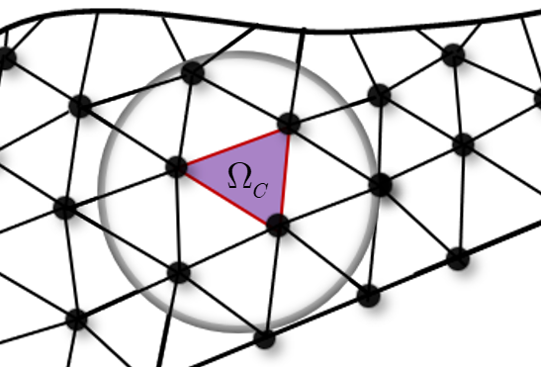
\includegraphics[scale=0.6]{figure/PHR/momentlisan.png}
%     \caption{背景积分单元示意图}\label{momentlisan}
% \end{figure}
\section{Hellinger-Reissner变分原理下的本质边界条件施加方法}
通过式(\ref{Pweakfrom})看出在四阶薄板问题上基于Hellinger-Reissner变分原理得到的弱形式中已经考虑了本质边界条件和自然边界条件。
为了更好的研究Hellinger-Reissner变分原理在求解薄板问题上的本质边界条件施加方法,此时将挠度离散表达式(\ref{w})和弯矩离散表达式(\ref{moment})代入到式(\ref{Pweakform2})中得到:
{\setlength\abovedisplayskip{0.5cm}
\setlength\belowdisplayskip{0.5cm}
\begin{equation}
\begin{split}
    &\int_{\Gamma}\sum_{I=1}^{N\!P}\Psi_I\delta{d_I}\mathcal{V}_{\alpha\beta}w_{,\alpha\beta}d\Gamma-\int_{\Gamma}\sum_{I=1}^{N\!P}\Psi_{I,n}\delta{d_I}\mathcal{M}_{\alpha\beta}w_{,\alpha\beta}d\Gamma+\sum_{I=1}^{N\!P}\Psi_I\delta{d_I}\mathcal{P}_{\alpha\beta}w_{,\alpha\beta}\vert_{x\in c}\\
    &-\int_{\Omega}\sum_{I=1}^{N\!P}\Psi_I\delta{d_I}\pmb{a}^T_{\alpha\beta,\alpha\beta}\tilde{\pmb q}d\Omega-\int_{\Gamma_w}\sum_{I=1}^{N\!P}\Psi_I\delta{d_I}\mathcal{V}_{\alpha\beta}w_{,\alpha\beta}d\Gamma\\
    &+\int_{\Gamma_{\theta}}\sum_{I=1}^{N\!P}\Psi_{I,n}\delta{d_I}\mathcal{M}_{\alpha\beta}w_{,\alpha\beta}d\Gamma
    -\sum_{I=1}^{N\!P}\Psi_I\delta{d_I}\mathcal{P}_{\alpha\beta}w_{,\alpha\beta}\vert_{x\in c_w}\\
    &=\sum_{I=1}^{N\!P}\int_{\Gamma_V}\Psi_I\delta{d_I}\bar{V}_{\pmb n}d\Gamma-\sum_{I=1}^{N\!P}\int_{\Gamma_M}\Psi_{I,n}\delta{d_I}\bar{M}_{\pmb{nn}}d\Gamma\\
    &+\sum_{I=1}^{N\!P}\Psi_I\delta{d_I}\bar{P}\vert_{x\in{c_P}}+\sum_{I=1}^{N\!P}\int_{\Omega}\Psi_I\delta{d_I}\bar{q}d\Omega
\end{split}
\end{equation}}
此时引入式(\ref{MVP1})并根据薄板问题线弹性本构关系式(\ref{Malphabeta})得出:
\begin{equation}\label{2}
\begin{split}
  -\sum_{C=1}^{N\!C}(\tilde{g}_{\alpha\beta I}^T-\tilde{g}_{\alpha\beta I}^T)\pmb a_{\alpha\beta}=\pmb{f}
\end{split}
\end{equation}
其中$\pmb{f}$为外力向量,具体表达式为:
\begin{equation}
\begin{split}
    \pmb{f}=\int_{\Gamma_V}\Psi_I\bar{V}_{\pmb n}d\Gamma-\int_{\Gamma_M}\Psi_{I,n}\bar{M}_{\pmb{nn}}d\Gamma+\Psi_I\bar{P}\vert_{x\in{c_P}}+\int_{\Omega}\Psi_I\bar{q}d\Omega
\end{split}
\end{equation}
此时,进一步将式(\ref{aalphabeta})中的$\pmb{a}_{\alpha\beta}$代入到式(\ref{2})中可以得到:
\begin{equation}
\begin{split}\label{Pzuzhuang}
    &-\sum_{C=1}^{N\!C}(\tilde{g}_{\alpha\beta I}^T-\bar{g}_{\alpha\beta I}^T)a_{\alpha\beta}\\
    &=\sum_{C=1}^{N\!C}(\tilde{g}_{\alpha\beta I}^T-\bar{g}_{\alpha\beta I}^T)D_{\alpha\beta\gamma\eta}\tilde{\pmb{G}}^{-1}(\sum_{J=1}^{N\!P}(\tilde{g}_{\gamma\eta J}-\bar{g}_{\gamma\eta J})d_I+\hat{g}_{\gamma\eta})\\
    &=\sum_{C=1}^{N\!C}\sum_{J=1}^{N\!P}D_{\alpha\beta\gamma\eta}\tilde{g}_{\alpha\beta I}^T\tilde{\pmb G}^{-1}\tilde{g}_{\gamma\eta J}d_J\\
    &+\sum_{C=1}^{N\!C}\sum_{J=1}^{N\!P}D_{\alpha\beta\gamma\eta}(-\bar{g}_{\alpha\beta I}^T\tilde{\pmb G}^{-1}\tilde{g}_{\gamma\eta J}-\tilde{g}_{\alpha\beta I}^T\tilde{\pmb G}^{-1}\tilde{g}_{\gamma\eta J})d_J\\
    &-(-\sum_{C=1}^{N\!C}D_{\alpha\beta\gamma\eta}\tilde{g}_{\alpha\beta I}^T\tilde{\pmb G}^{-1}\hat{g}_{\gamma\eta })\\
    &+\sum_{C=1}^{N\!C}\sum_{J=1}^{N\!P}D_{\alpha\beta\gamma\eta}\bar{g}_{\alpha\beta I}^T\tilde{\pmb G}^{-1}\tilde{g}_{\gamma\eta J}d_J\\
    &-\sum_{C=1}^{N\!C}D_{\alpha\beta\gamma\eta}\bar{g}_{\alpha\beta I}^T\tilde{\pmb G}^{-1}\hat{g}_{\gamma\eta }
\end{split}
\end{equation}
通过引入式(\ref{PG})、(\ref{PTPSI})对式(\ref{Pzuzhuang})中的第一项进行推导可以得到:
\begin{equation}
\begin{split}
    &\sum_{C=1}^{N\!C}D_{\alpha\beta\gamma\eta}\tilde{g}_{\alpha\beta I}^T\tilde{\pmb G}^{-1}\tilde{g}_{\gamma\eta J}\\
    &=\sum_{C=1}^{N\!C}D_{\alpha\beta\gamma\eta}\tilde{g}_{\alpha\beta I}^T\tilde{\pmb G}^{-1}\int_{\Omega_C}\tilde{\pmb q}\tilde{\pmb q}^Td\Omega\tilde{\pmb G}^{-1}\tilde{g}_{\gamma\eta J}\\
    &=\sum_{C=1}^{N\!C}D_{\alpha\beta\gamma\eta}\int_{\Omega_C}\tilde{g}_{\alpha\beta I}^T\tilde{\pmb G}^{-1}\tilde{\pmb q}\tilde{\pmb q}^T\tilde{\pmb G}^{-1}\tilde{g}_{\gamma\eta J}d\Omega \\
    &=\int_{\Omega}\tilde{\Psi}_{I,\alpha\beta}D_{\alpha\beta\gamma\eta}\tilde{\Psi}_{J,\gamma\eta}d\Omega \\
    &=\pmb{K}
\end{split}
\end{equation}
\newpage
通过引入式(\ref{PTPSI})、(\ref{MVP1})对式(\ref{Pzuzhuang})中的第二项进行推导可以得到:
\begin{equation}
\begin{split}
    &-\sum_{C=1}^{N\!C}D_{\alpha\beta\gamma\eta}(\bar{g}_{\alpha\beta I}^T\tilde{\pmb G}^{-1}\tilde{g}_{\gamma\eta J}+\tilde{g}_{\alpha\beta I}^T\tilde{\pmb G}^{-1}\tilde{g}_{\gamma\eta J})\\
    &=\sum_{C=1}^{N\!C}D_{\alpha\beta\gamma\eta}\int_{{\Gamma_w}\cap{\Gamma_C}}\Psi_I(n_{\alpha}
    \tilde{\pmb q}_{,\beta}^T\tilde{\pmb G}^{-1}\tilde{g}_{\gamma\eta J}+\tilde{\pmb q}_{,\xi}^T\tilde{\pmb G}^{-1}\tilde{g}_{\gamma\eta J}s_{\alpha}n_{\beta}s_{\xi})d\Gamma\\
    &+\sum_{C=1}^{N\!C}D_{\alpha\beta\gamma\eta}\int_{{\Gamma_w}\cap{\Gamma_C}}(n_{\gamma}
    \tilde{g}_{\alpha\beta I}^T\tilde{\pmb G}^{-1}\tilde{\pmb q}_{,\eta}+\tilde{g}_{\alpha\beta I}^T
    \tilde{\pmb G}^{-1}\tilde{\pmb q}_{,\xi}s_{\gamma}n_{\eta}s_{\xi})\Psi_Jd\Gamma\\
    &-\sum_{C=1}^{N\!C}D_{\alpha\beta\gamma\eta}\int_{{\Gamma_{\theta}}\cap{\Gamma_C}}\Psi_{I,n}
    \tilde{\pmb q}^T\tilde{\pmb G}^{-1}\tilde{g}_{\gamma\eta J}n_{\alpha}n_{\beta}d\Gamma
    -\sum_{C=1}^{N\!C}D_{\alpha\beta\gamma\eta}\int_{{\Gamma_{\theta}}\cap{\Gamma_C}}
    \tilde{g}_{\alpha\beta I}^T\tilde{\pmb G}^{-1}\tilde{\pmb q}n_{\gamma}n_{
    \eta}\Psi_{J,n}d\Gamma\\
    &-\sum_{C=1}^{N\!C}D_{\alpha\beta\gamma\eta}[[\Psi_I\tilde{\pmb q}^T\tilde{\pmb G}^{-1}\tilde{g}_{\gamma\eta J}n_{\alpha}s_{\beta}]]_{x\in{c_w}\cap{c_C}}
    -\sum_{C=1}^{N\!C}D_{\alpha\beta\gamma\eta}[[\tilde{g}_{\alpha\beta I}^T\tilde{\pmb G}^{-1}\tilde{\pmb q}n_{\gamma}s_{\eta}\Psi_J]]_{x\in{c_w}\cap{c_C}}\\
    &=-\sum_{C=1}^{N\!C}\int_{{\Gamma_w}\cap{\Gamma_C}}\Psi_I(-D_{\alpha\beta\gamma\eta}(n_{\alpha}\frac{\partial}{\partial x_{\beta}}+s_{\alpha}n_{\beta}s_{\xi}\frac{\partial}{\partial x_{\xi}}))\tilde{\Psi}_{J,\gamma\eta}d\Gamma\\
    &-\sum_{C=1}^{N\!C}\int_{{\Gamma_w}\cap{\Gamma_C}}(-D_{\alpha\beta\gamma\eta}(n_{\gamma}\frac{\partial}{\partial x_{\eta}}+s_{\gamma}n_{\eta}s_{\xi}\frac{\partial}{\partial x_{\xi}}))\tilde{\Psi}_{I,\alpha\beta}\Psi_Jd\Gamma\\
    &+\sum_{C=1}^{N\!C}\int_{{\Gamma_{\theta}}\cap{\Gamma_C}}\Psi_{I,n}(-D_{\alpha\beta\gamma\eta}n_{\alpha}n_{\beta})\tilde{\Psi}_{J,\gamma\eta}d\Gamma
    +\sum_{C=1}^{N\!C}\int_{{\Gamma_{\theta}}\cap{\Gamma_C}}(-D_{\alpha\beta\gamma\eta}n_{\gamma}n_{\eta})\tilde{\Psi}_{I,\alpha\beta}\Psi_{J,n}d\Gamma\\
    &+\sum_{C=1}^{N\!C}[[\Psi_I(-D_{\alpha\beta\gamma\eta}n_{\gamma}s_{\eta})\tilde{\Psi}_{J,\gamma\eta}]]_{x\in{c_w}\cap{c_C}}+\sum_{C=1}^{N\!C}[[(-D_{\alpha\beta\gamma\eta}n_{\gamma}s_{\eta})\tilde{\Psi}_{I,\alpha\beta}\Psi_J]]_{x\in{c_w}\cap{c_C}}\\
    &=-\int_{\Gamma_w}\Psi_I\mathcal{V}_{\alpha\beta}\tilde{\Psi}_{J,\alpha\beta}d\Gamma+\int_{\Gamma_{\theta}}\Psi_{I,n}\mathcal{M}_{\alpha\beta}\tilde{\Psi}_{J,\alpha\beta}d\Gamma+[[\Psi_I\mathcal{P}_{\alpha\beta}\tilde{\Psi}_{J,\alpha\beta}]]_{x\in{c_w}}\\
    &-\int_{\Gamma_w}\mathcal{V}_{\alpha\beta}\tilde{\Psi}_{I,\alpha\beta}\Psi_Jd\Gamma+\int_{\Gamma_{\theta}}\mathcal{M}_{\alpha\beta}\tilde{\Psi}_{I,\alpha\beta}\Psi_{J,n}d\Gamma+[[\mathcal{P}_{\alpha\beta}\tilde{\Psi}_{I,\alpha\beta}\Psi_J]]_{x\in{c_w}}\\
    &=\tilde{\pmb K}
\end{split}
\end{equation}
\newpage
通过引入式(\ref{PTPSI})、(\ref{MVP1})对式(\ref{Pzuzhuang})中的第三项进行推导可以得到:
\begin{equation}
\begin{split}
    &-\sum_{C=1}^{N\!C}D_{\alpha\beta\gamma\eta}\tilde{g}^T_{\alpha\beta I}\tilde{\pmb G}^{-1}\hat{g}_{\gamma\eta}\\
    &=\sum_{C=1}^{N\!C}D_{\alpha\beta\gamma\eta}\int_{{\Gamma_w}\cap{\Gamma_C}}(n_{\gamma}
    \tilde{g}_{\alpha\beta I}^T\tilde{\pmb G}^{-1}\tilde{\pmb q}_{,\eta}+\tilde{g}_{\alpha\beta I}^T
    \tilde{\pmb G}^{-1}\tilde{\pmb q}_{,\xi}s_{\gamma}n_{\eta}s_{\xi})\bar{w}d\Gamma\\
    &-\sum_{C=1}^{N\!C}D_{\alpha\beta\gamma\eta}\int_{{\Gamma_{\theta}}\cap{\Gamma_{C}}}\tilde{g}^T_{\alpha\beta I}\tilde{\pmb G}^{-1}\tilde{\pmb q}n_{\gamma}n_{\eta}\bar{\theta}_nd\Gamma-[[\tilde{g}_{\alpha\beta I}\tilde{\pmb G}^{-1}\tilde{\pmb q}n_{\gamma}s_{\eta}\bar{w}]]_{x\in{c_w}\cap{c_C}}\\
    &=-\sum_{C=1}^{N\!C}\int_{{\Gamma_w}\cap{\Gamma_C}}(-D_{\alpha\beta\gamma\eta}(n_{\gamma}\frac{\partial}{\partial x_{\eta}}+s_{\gamma}n_{\eta}s_{\xi}\frac{\partial}{\partial x_{\xi}}))\tilde{\Psi}_{I,\alpha\beta}\bar{w}d\Gamma\\
    &+\sum_{C=1}^{N\!C}\int_{{\Gamma_{\theta}}\cap{\Gamma_C}}(-D_{\alpha\beta\gamma\eta}n_{\gamma}n_{\eta})\tilde{\Psi}_{I,\alpha\beta}\bar{\theta}_{\pmb n}d\Gamma-[[(-D_{\alpha\beta\gamma\eta}n_{\gamma}s_{\eta}\tilde{\Psi}_{I,\alpha\beta}\bar{w})]]_{x\in{c_w}\cap{c_C}}\\
    &=\int_{\Gamma_w}\mathcal{V}_{\alpha\beta}\tilde{\Psi}_{I,\alpha\beta}\bar{w}d\Gamma+\int_{\Gamma_{\theta}}\mathcal{M}_{\alpha\beta}\tilde{\Psi}_{I,\alpha\beta}\bar{\theta}_{\pmb n}d\Gamma+[[\mathcal{P}_{\alpha\beta}\tilde{\Psi}_{I,\alpha\beta}\bar{w}]]_{x\in{c_w}}\\
    &=\tilde{\pmb f}
\end{split}
\end{equation}
通过引入式(\ref{PBPSI})、(\ref{MVP1})对式(\ref{Pzuzhuang})中的第四项进行推导可以得到:
\begin{equation}
\begin{split}
    &\sum_{C=1}^{N\!C}D_{\alpha\beta\gamma\eta}\bar{g}_{\alpha\beta I}^T\tilde{\pmb G}^{-1}\tilde{g}_{\gamma\eta J}\\
    &=\sum_{C=1}^{N\!C}D_{\alpha\beta\gamma\eta}\int_{{\Gamma_w}\cap{\Gamma_C}}(n_{\gamma}
    \bar{g}_{\alpha\beta I}^T\tilde{\pmb G}^{-1}\bar{\pmb q}_{,\eta}+\tilde{g}_{\alpha\beta I}^T
    \tilde{\pmb G}^{-1}\tilde{\pmb q}_{,\xi}s_{\gamma}n_{\eta}s_{\xi})\Psi_Jd\Gamma\\
    &-\sum_{C=1}^{N\!C}D_{\alpha\beta\gamma\eta}\int_{{\Gamma_{\theta}}\cap{\Gamma_C}}
    \bar{g}_{\alpha\beta I}^T\tilde{\pmb G}^{-1}\tilde{\pmb q}n_{\gamma}n_{
    \eta}\Psi_{J,n}d\Gamma
    -\sum_{C=1}^{N\!C}D_{\alpha\beta\gamma\eta}[[\bar{g}_{\alpha\beta I}^T\tilde{\pmb G}^{-1}\tilde{\pmb q}n_{\gamma}s_{\eta}\Psi_J]]_{x\in{c_w}\cap{c_C}}\\
    &=\sum_{C=1}^{N\!C}\int_{{\Gamma_w}\cap{\Gamma_C}}(-D_{\alpha\beta\gamma\eta}(n_{\gamma}\frac{\partial}{\partial x_{\eta}}+s_{\gamma}n_{\eta}s_{\xi}\frac{\partial}{\partial x_{\xi}}))\bar{\Psi}_{I,\alpha\beta}\Psi_Jd\Gamma\\
    &-\sum_{C=1}^{N\!C}\int_{{\Gamma_{\theta}}\cap{\Gamma_C}}(-D_{\alpha\beta\gamma\eta}n_{\gamma}n_{\eta})\bar{\Psi}_{I,\alpha\beta}\Psi_{J,n}d\Gamma
    -[[(-D_{\alpha\beta\gamma\eta}n_{\gamma}s_{\eta})\bar{\Psi}_{I,\alpha\beta}\Psi_J]]_{x\in{c_w}\cap{c_C}}\\
    &=\int_{\Gamma_w}\mathcal{V}_{\alpha\beta}\bar{\Psi}_{I,\alpha\beta}\Psi_Jd\Gamma-\int_{\Gamma_{\theta}}\mathcal{M}_{\alpha\beta}\bar{\Psi}_{I,\alpha\beta}\Psi_{J,n}d\Gamma+[[\mathcal{P}_{\alpha\beta}\bar{\Psi}_{I,\alpha\beta}\Psi_J]]_{x\in{c_w}}\\
    &=\bar{\pmb K}
\end{split}
\end{equation}
通过引入式(\ref{PBPSI})、(\ref{MVP1})对式(\ref{Pzuzhuang})中的第五项进行推导可以得到:
\begin{equation}
 \begin{split}
    &-\sum_{C=1}^{N\!C}D_{\alpha\beta\gamma\eta}\bar{g}_{\alpha\beta I}^T\tilde{\pmb G}^{-1}\hat{g}_{\gamma\eta }\\
    &=\sum_{C=1}^{N\!C}D_{\alpha\beta\gamma\eta}\int_{{\Gamma_w}\cap{\Gamma_C}}(n_{\eta}
    \bar{g}_{\alpha\beta I}^T\tilde{\pmb G}^{-1}\tilde{\pmb q}_{,\gamma}+\bar{g}_{\alpha\beta I}^T
    \tilde{\pmb G}^{-1}\tilde{\pmb q}_{,\xi}s_{\gamma}n_{\eta}s_{\xi})\bar{w}d\Gamma\\
    &-\sum_{C=1}^{N\!C}D_{\alpha\beta\gamma\eta}\int_{{\Gamma_{\theta}}\cap{\Gamma_{C}}}\bar{g}^T_{\alpha\beta I}\tilde{\pmb G}^{-1}\tilde{\pmb q}n_{\gamma}n_{\eta}\bar{\theta}_nd\Gamma-[[\bar{g}_{\alpha\beta I}\tilde{\pmb G}^{-1}\tilde{\pmb q}n_{\gamma}s_{\eta}\bar{w}]]_{x\in{c_w}\cap{c_C}}\\
    &=\sum_{C=1}^{N\!C}\int_{{\Gamma_w}\cap{\Gamma_C}}(-D_{\alpha\beta\gamma\eta}(n_{\gamma}\frac{\partial}{\partial x_{\eta}}+s_{\gamma}n_{\eta}s_{\xi}\frac{\partial}{\partial x_{\xi}}))\bar{\Psi}_{I,\alpha\beta}\bar{w}d\Gamma\\
    &-\sum_{C=1}^{N\!C}\int_{{\Gamma_{\theta}}\cap{\Gamma_C}}(-D_{\alpha\beta\gamma\eta}n_{\gamma}n_{\eta})\bar{\Psi}_{I,\alpha\beta}\bar{\theta}_{\pmb n}d\Gamma-[[(-D_{\alpha\beta\gamma\eta}n_{\gamma}s_{\eta}\bar{\Psi}_{I,\alpha\beta}\bar{w})]]_{x\in{c_w}\cap{c_C}}\\
    &=\int_{\Gamma_w}\mathcal{V}_{\alpha\beta}\bar{\Psi}_{I,\alpha\beta}\bar{w}d\Gamma+\int_{\Gamma_{\theta}}\mathcal{M}_{\alpha\beta}\bar{\Psi}_{I,\alpha\beta}\bar{\theta}_{\pmb n}d\Gamma+[[\mathcal{P}_{\alpha\beta}\bar{\Psi}_{I,\alpha\beta}\bar{w}]]_{x\in{c_w}}\\
    &=\bar{\pmb f}
\end{split}
\end{equation}
通过上述所进行的推导,式(\ref{Pzuzhuang})通过化简可以得到:
\begin{equation}
\begin{split}
    &-\sum_{C=1}^{N\!C}(\tilde{g}_{\alpha\beta I}^T-\bar{g}_{\alpha\beta I}^T)a_{\alpha\beta}\\
    &=\sum_{C=1}^{N\!C}(\tilde{g}_{\alpha\beta I}^T-\bar{g}_{\alpha\beta I}^T)D_{\alpha\beta\gamma\eta}\tilde{\pmb{G}}^{-1}(\sum_{J=1}^{N\!P}(\tilde{g}_{\gamma\eta J}-\bar{g}_{\gamma\eta J})d_I+\hat{g}_{\gamma\eta})\\
    &=\sum_{J=1}^{N\!P}(\pmb{K}+\tilde{\pmb K}+\bar{\pmb K})d_J-\tilde{\pmb f}-\bar{\pmb f}
\end{split}
\end{equation}
将上式带入到式(\ref{2})得到薄板问题的离散平衡方程为:
\begin{equation}\label{equationP}
\begin{split}
    (\pmb{K}+\tilde{\pmb K}+\bar{\pmb K})\pmb{d}=\pmb{f}+\tilde{\pmb f}+\bar{\pmb f}
\end{split}
\end{equation}\par
同样,Hellinger-Reissner变分原理下的薄板问题离散平衡控制方程式中的修正变分项$\tilde{K}_{IJ}$、$\tilde{f}_I$和满足变分一致性的Nitsche法中的$K_{IJ}^n$、$f_I^n$相比,用再生光滑梯度$\tilde{\pmb{B}}_I$替代传统无网格形函数梯度$\pmb{B}_I$,进而提高计算效率。
Hellinger-Reissner变分原理下的离散平衡控制方程式中的稳定项$\bar{K}_{IJ}$、$\bar{f}_I$和传统的Nitshche法中的$K^{\alpha}_{IJ}$、$f^{\alpha}_I$相比,无限额外施加人工参数,提高计算精度。\par
为了保证离散弱形式的变分一致性在求解式(\ref{equationP})的过程中,同样引入的数值积分在求解的各个过程中也需要保存一致。
如图(\ref{Pintegralscheme})所示,求解薄板问题时基于Hellinger-Reissner变分原理下的本质边界条件施加方法需要两套数值积分点\cite{}。
\begin{figure}[H]
    \centering
    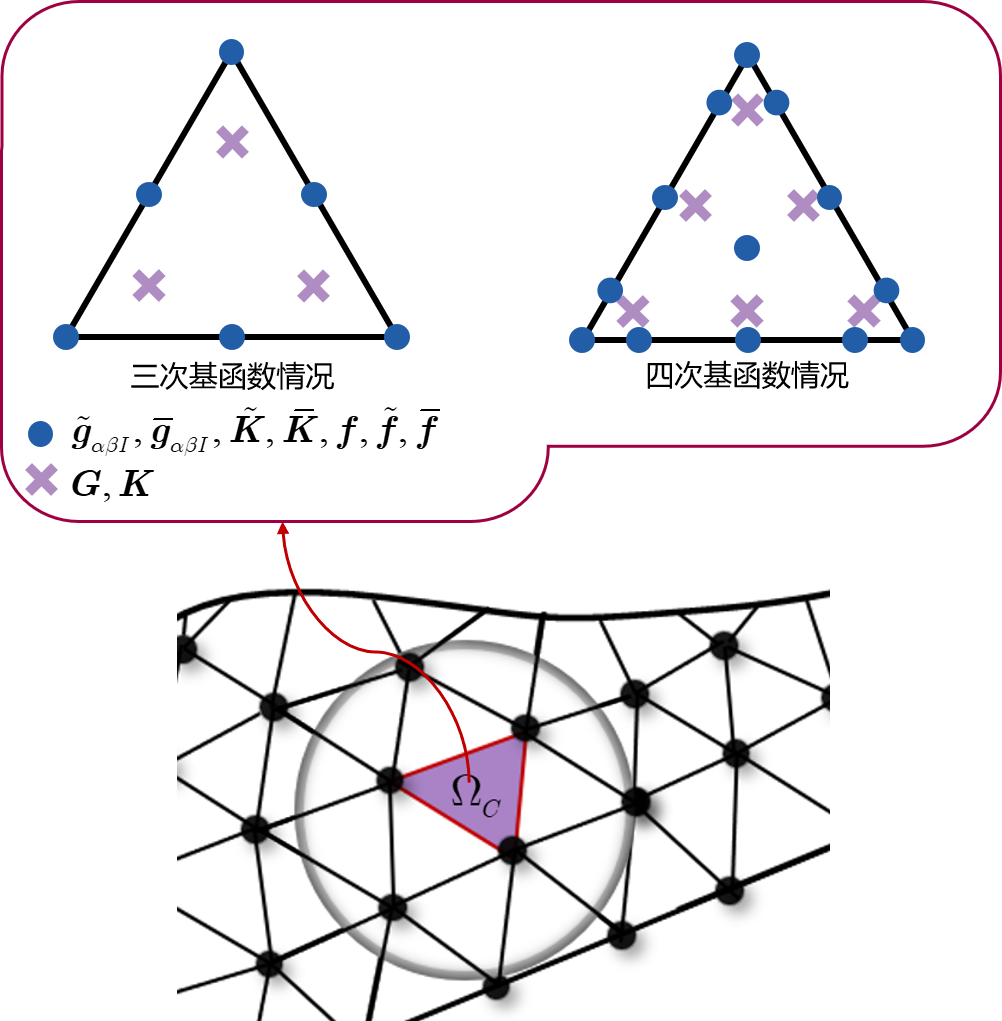
\includegraphics[scale=0.5]{figure/PHR/Pintegralscheme.png}
    \caption{优化的数值积分方案}\label{Pintegralscheme}
\end{figure}
\section{数值算例}
\subsection{分片实验}
关于薄板问题,采用二次、三次和四次高阶薄板分片实验验证采用传统高斯积分法和再生光滑梯度积分法的不同本质边界条件施加方法是否和二阶弹性力学问题相同
满足积分约束条件。此时分片实验考虑求解域为$\Omega=(0,1)\otimes(0,1)$的正方形薄板,求解域的四边施加本质边界条件。其分片实验的精确解如下:
\begin{equation}
\begin{split}
    w(\pmb{x})=\begin{cases}
        x_1^2+2x_1x_2\quad &\text{二次分片实验}\\
        x_1^3+2x_1^2x_2+3x_1x_2^2\quad &\text{三次分片实验}\\
        x_1^4+2x_1^3x_2+3x_1^2x_2^2+4x_1x_2^3\quad&\text{四次分片实验}
    \end{cases}
\end{split}
\end{equation}\par
如图所示(\ref{fenpian}),薄板问题的分片实验由49个无网格节点进行离散。针对三次基函数的无网格近似,采用二次和三次分片实验进行测试,核函数的相对影响域在三次基函数的情况下设为3.5;
而四次基函数的无网格近似采用三次和四次分片实验进行测试,核函数的相对影响域在四次基函数的情况下设为4.5。\par
\begin{figure}[H]
    \centering
    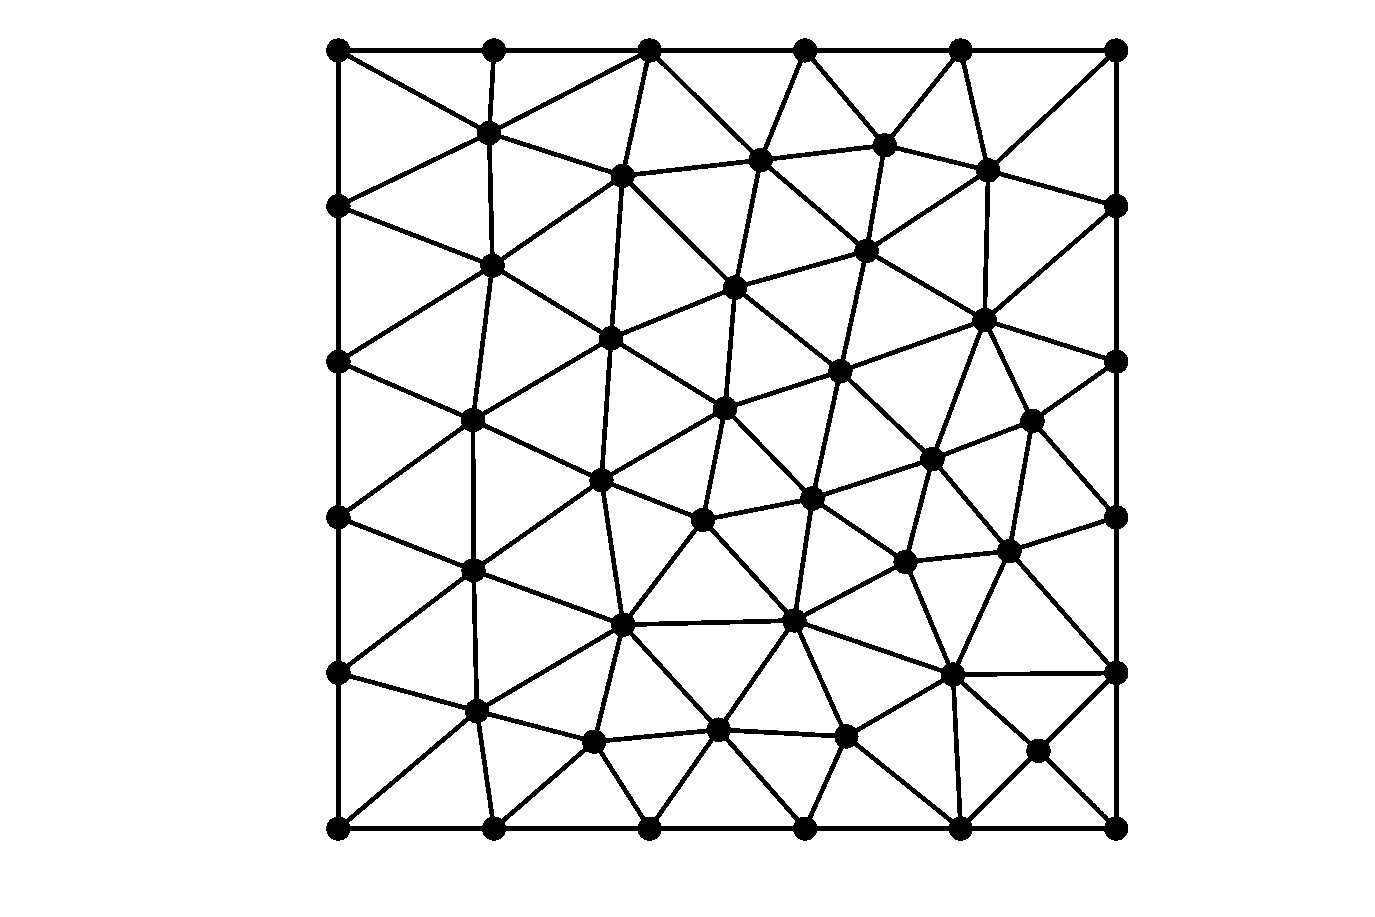
\includegraphics[scale=0.7]{figure/PHR/fenpian.png}
    \caption{分片实验无网格离散模型}\label{fenpian}
\end{figure}
为了更好的对比所提方法的计算精度,针对四阶薄板问题分别采用如下位移误差$L_2-\text{Error}$和能量误差$H_i-\text{Error}$进行分析:
\begin{equation}
\begin{split}
    &L_2-\text{Error}=\frac{\sqrt{\int_{\Omega}(w-w^h)^2d\Omega}}{\sqrt{\int_{\Omega}w^2d\Omega}}\\
    &H_i-\text{Error}=\frac{\sum_{j=0}^{i}\sqrt{\int_{\Omega}(w_{,\alpha_1\dotsb \alpha_j}-w_{,\alpha_1\dotsb \alpha_j})^2}d\Omega}{\sum_{j=0}^{i}\sqrt{\int_{\Omega}w_{,\alpha_1\dotsb \alpha_j}w_{,\alpha_1\dotsb \alpha_j}d\Omega}}
\end{split}
\end{equation}\par
针对薄板问题,三次基函数的求解计算时高斯积分法“GI”的求解域$\Omega$的积分采用13点高斯积分,边界$\Gamma$积分采用3点高斯积分;
四次基函数的求解计算时高斯积分法“GI”的求解域$\Omega$的积分采用16点高斯积分,边界$\Gamma$积分采用5点高斯积分;
再生光滑梯度积分法“RKGSI”计算时采用的积分点数和高斯积分法一致。三次和四次基函数的无网格分片试验结果如下表:
\newpage
\begin{table}[H]
    \caption{\textbf{三次基函数无网格法分片实验结果}}
    \centering\label{cubic}
   \begin{tabular}{ccccc}
   \toprule
   &$\quad$ &二次分片实验 &$\quad$ &三次分片实验\\
   \midrule
   &$L_2$-Error$\quad$&$H_2$-Error&$L_2$-Error$\quad$&$H_2$-Error\\
   \midrule
   GI-Penalty&$4.27\times10^{-2}$&$3.82\times10^{-1}$&$9.54\times10^{-2}$&$5.12\times10^{-1}$\\
   GI-Nitsche&$4.09\times10^{-2}$&$3.75\times10^{-1}$&$9.50\times10^{-2}$&$5.05\times10^{-1}$\\
  RKGSI-Penalty&$4.60\times10^{-2}$&$3.86\times10^{-1}$&$1.07\times10^{-1}$&$5.40\times10^{-1}$\\
  RKGSI-Nitsche&$5.67\times10^{-14}$&$2.18\times10^{-12}$&$5.21\times10^{-14}$&$1.20\times10^{-12}$\\
  RKGSI-HR&$5.58\times10^{-15}$&$4.56\times10^{-13}$&$3.66\times10^{-15}$&$2.70\times10^{-13}$\\
   \bottomrule
   \end{tabular}
   \end{table}
\begin{table}[H]
    \caption{\textbf{四次基函数无网格法分片实验结果}}
    \centering\label{quartic}
   \begin{tabular}{ccccc}
   \toprule
   &$\quad$ &三次分片实验 &$\quad$ &四次分片实验\\
   \midrule
   &$L_2$-Error$\quad$&$H_1$-Error&$L_2$-Error$\quad$&$H_1$-Error\\
   \midrule
   GI-Penalty&$1.08\times10^{-1}$&$5.44\times10^{-1}$&$1.84\times10^{-1}$&$6.32\times10^{-1}$\\
   GI-Nitsche&$1.07\times10^{-1}$&$5.45\times10^{-1}$&$1.84\times10^{-1}$&$6.34\times10^{-1}$\\
  RKGSI-Penalty&$1.06\times10^{-1}$&$5.40\times10^{-1}$&$1.84\times10^{-1}$&$6.26\times10^{-1}$\\
  RKGSI-Nitsche&$2.82\times10^{-13}$&$4.99\times10^{-12}$&$3.03\times10^{-13}$&$3.33\times10^{-12}$\\
  RKGSI-HR&$1.68\times10^{-14}$&$2.33\times10^{-12}$&$4.40\times10^{-14}$&$1.57\times10^{-12}$\\
\bottomrule
\end{tabular}
\end{table}\par
表(\ref{cubic})和表(\ref{quartic})分别表示具有三次、四次基函数无网格法的薄板分片试验结果,从表中可以明显的看出,由于缺乏变分一致性
传统高斯积分法“GI-Penalty”、“GI-Nitsche”和罚函数法“RKGSI-Penalty”都无法通过分片试验。只有满足变分一致性的再生光滑梯度积分法的“RKGSI-Nitsche”法和
本章提出的Hellinger-Ressiner变分原理的本质边界条件施加方案“RKGSI-HR”法可以通过分片试验,满足积分约束条件。
\subsection{简支方板问题}
如图(\ref{rectangular})所示,一简支方板的中性面区域为$\Omega=(0,1)\otimes(0,1)$,此时$\Omega$的长为$a=1$宽为$b=1$,材料系数分别为弯曲刚度$\bar{D}=1$、$\nu=0.3$。板面内分布如图所示纵向荷载:
\begin{equation}
\begin{split}
    \bar q=-\bar D(\frac{\pi^2}{a^2}+\frac{\pi^2}{b^2})sin(\frac{\pi}{a}x)sin(\frac{\pi}{b}y)
\end{split}
\end{equation}
该简支方板问题的精确解为:
\begin{equation}
\begin{split}
    w=-sin(\frac{\pi}{a}x)sin(\frac{\pi}{b}y)
\end{split}
\end{equation}
\begin{figure}[H]
\centering
    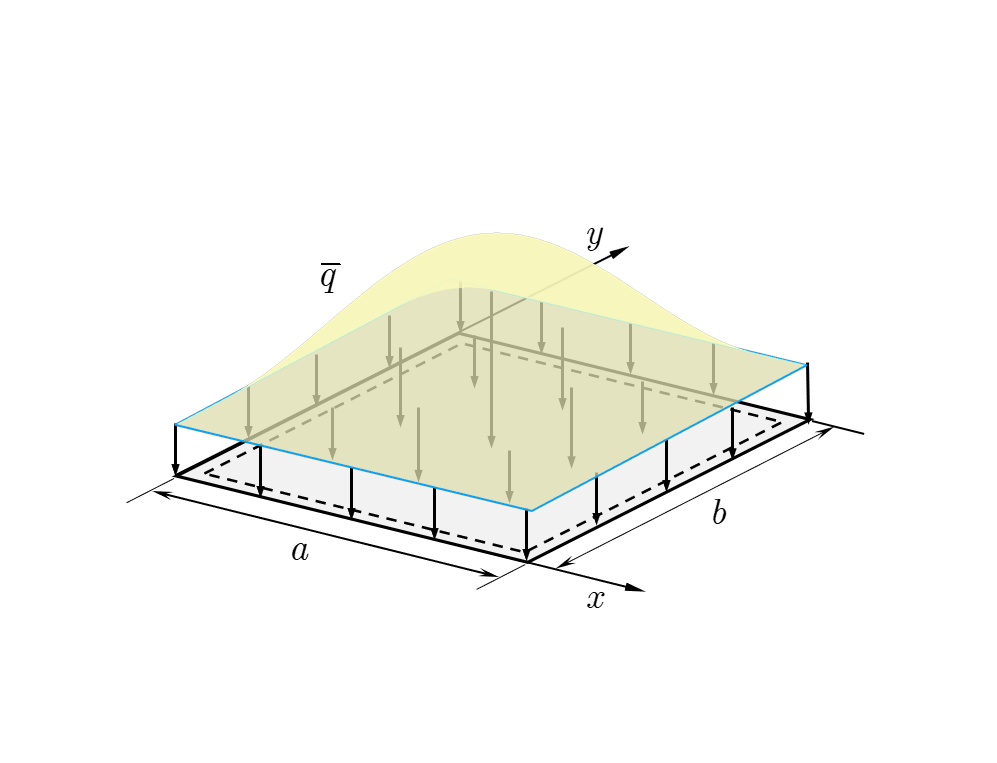
\includegraphics[scale=0.7]{figure/PHR/R/rectangular.png}
    \caption{简支方板问题模型}\label{rectangular}
\end{figure}
如图所示(\ref{rectangularmsh}),简支方板求解域采用均布的$11\times 11$、$21\times 21$、$41\times 41$、$81\times 81$的四个疏密不同的节点进行离散。
此时对于采用三次基函数的简支方板问题其相对影响域取为3.5,采用四次基函数时其相对影响域则取为4.5。\par

\begin{figure}[H]
\centering
      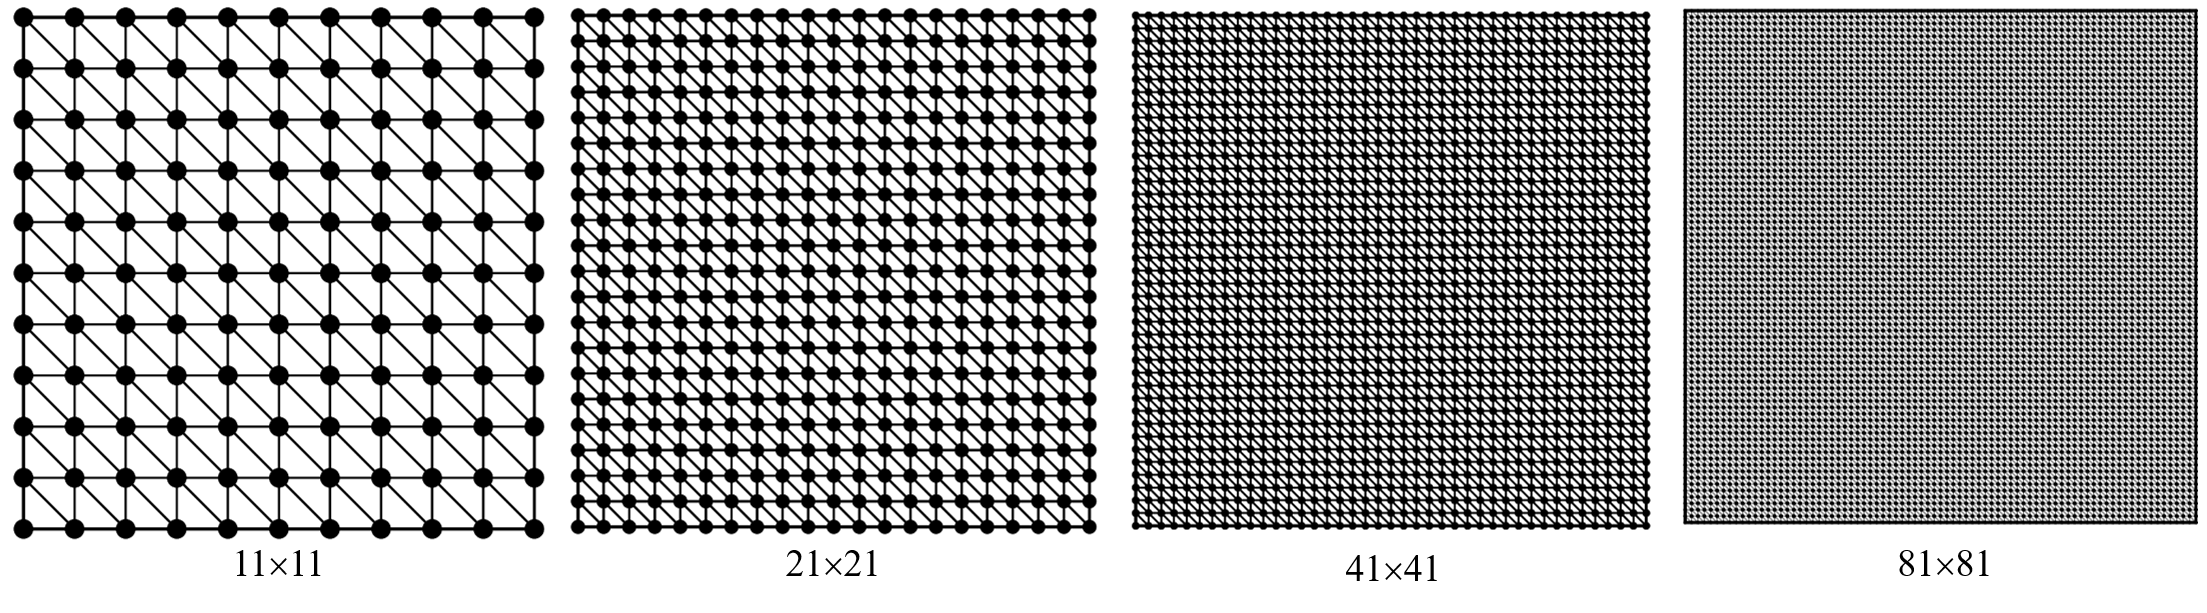
\includegraphics[scale=0.4]{figure/PHR/R/rectangularmsh.png}
    \caption{简支方板问题节点离散}\label{rectangularmsh}
\end{figure}
 图(\ref{RCLH})和图(\ref{RQLH})分别为简支方板问题在三次基函数和四次基函数时的位移误差和能量误差对比图。从图中可以明显看出即使采用高阶高斯积分法“GI”如三次基函数的13点高斯积分法和四次基函数的16点高斯积分,
计算精度都低于再生光滑梯度法“RKGSI”,并且和同样不满足变分一致性的罚函数法一样都无法达到理论误差收敛率。而“RKGSI-Nitsche”和“RKGSI-HR”法不管是在三次基函数还是四次基函数时都达到了误差收敛率。
图(\ref{RCcputime})、(\ref{RQcputime})是简支方板问题在三次基函数和四次基函数时分别计算节点数和与使用“GI”和“RKGSI”不同数值积分方法时的效率图。从整体来看采用“RKGSI”时的计算效率在三次基函数和四次基函数时都明显高于“GI”。  

\begin{figure}[H]
    \centering
    \begin{subcaptiongroup}
    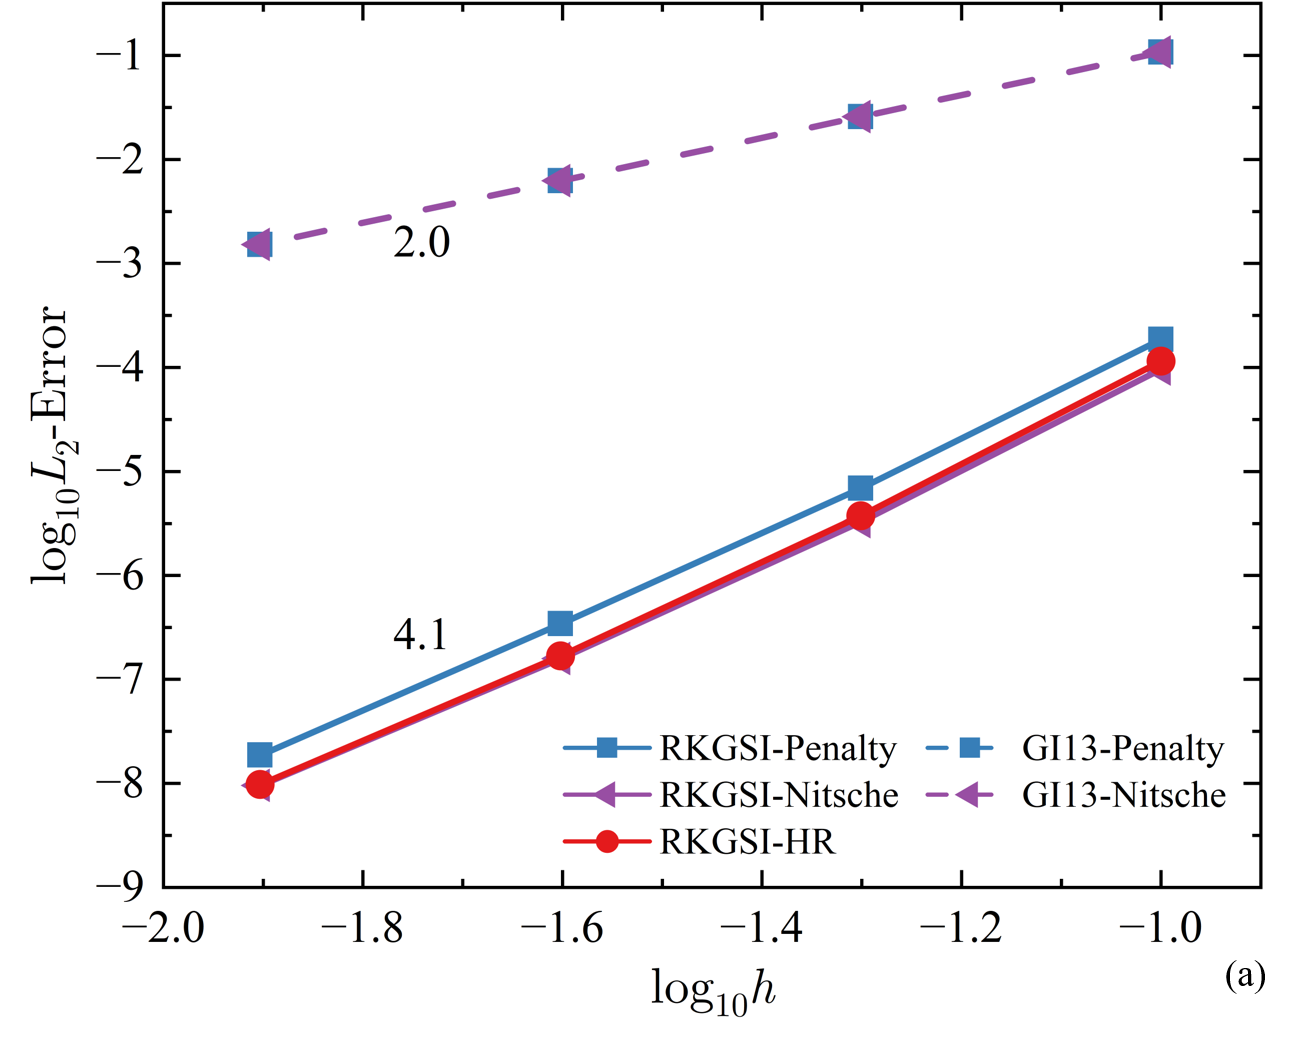
\includegraphics[width=0.49\textwidth]{figure/PHR/R/CL2.png}
    \phantomcaption\label{CL2}
    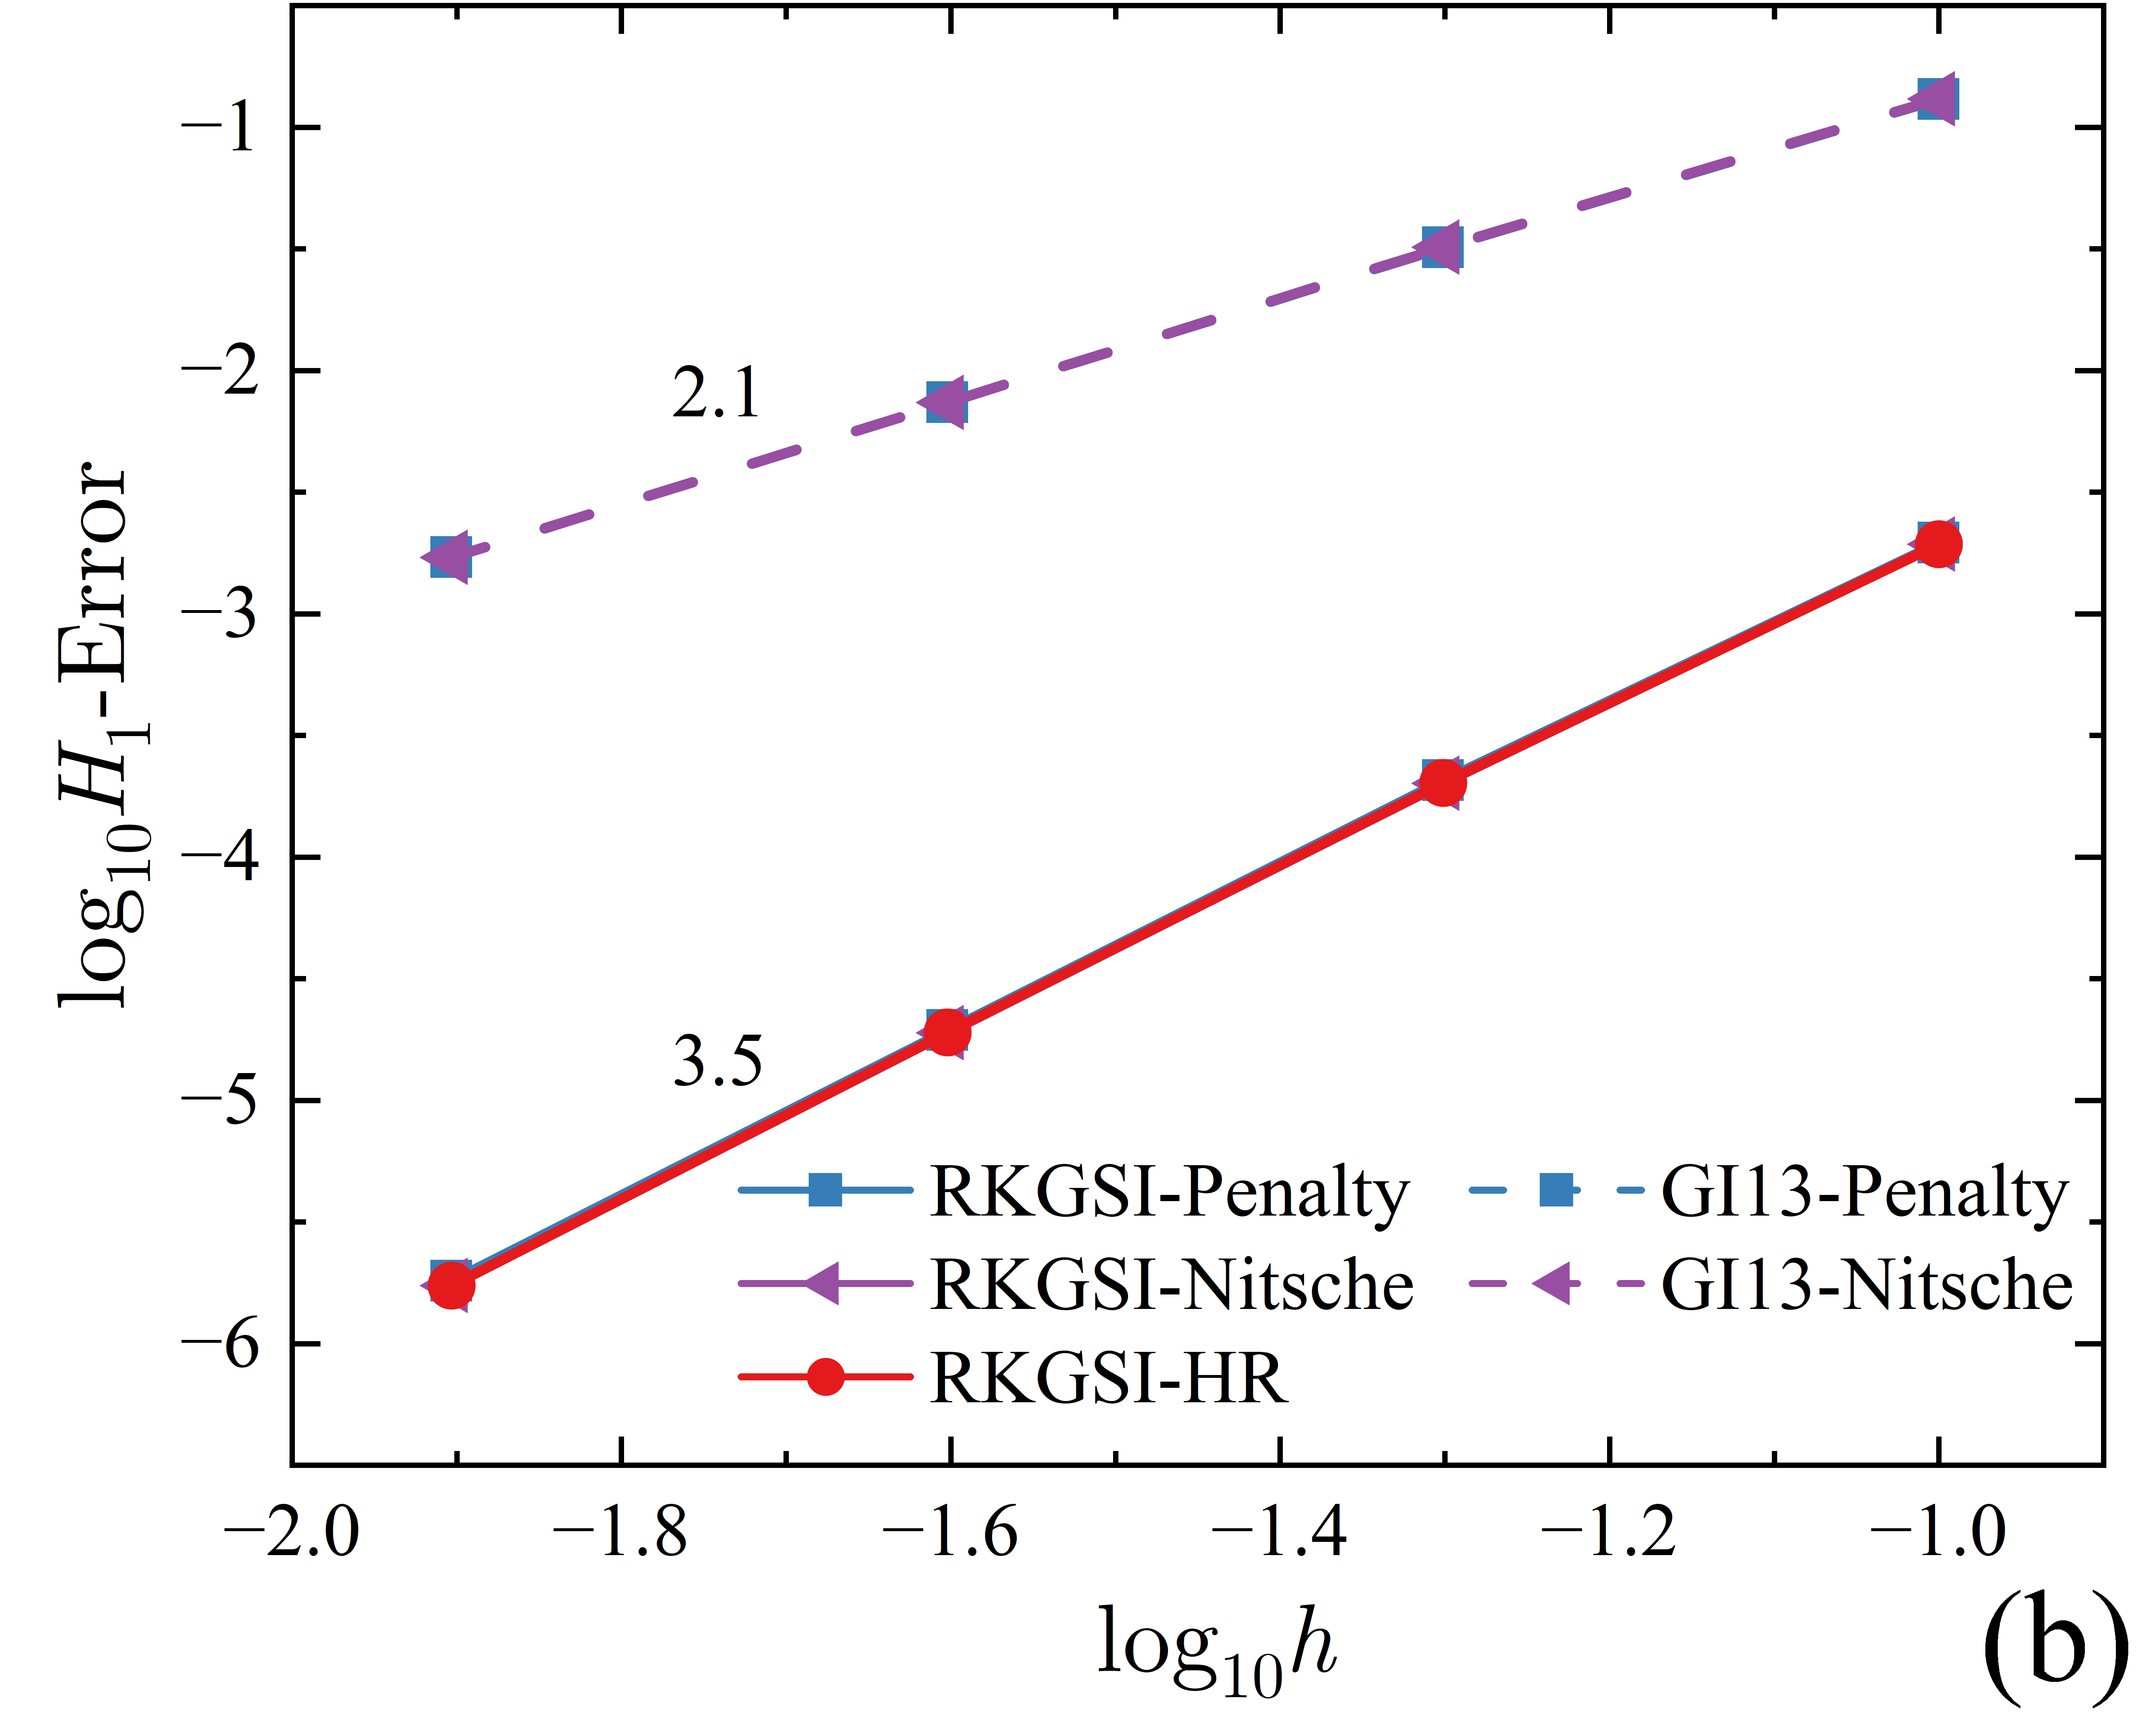
\includegraphics[width=0.49\textwidth]{figure/PHR/R/CH1.png}
    \phantomcaption\label{CH1}
    \end{subcaptiongroup}
    \begin{subcaptiongroup}
    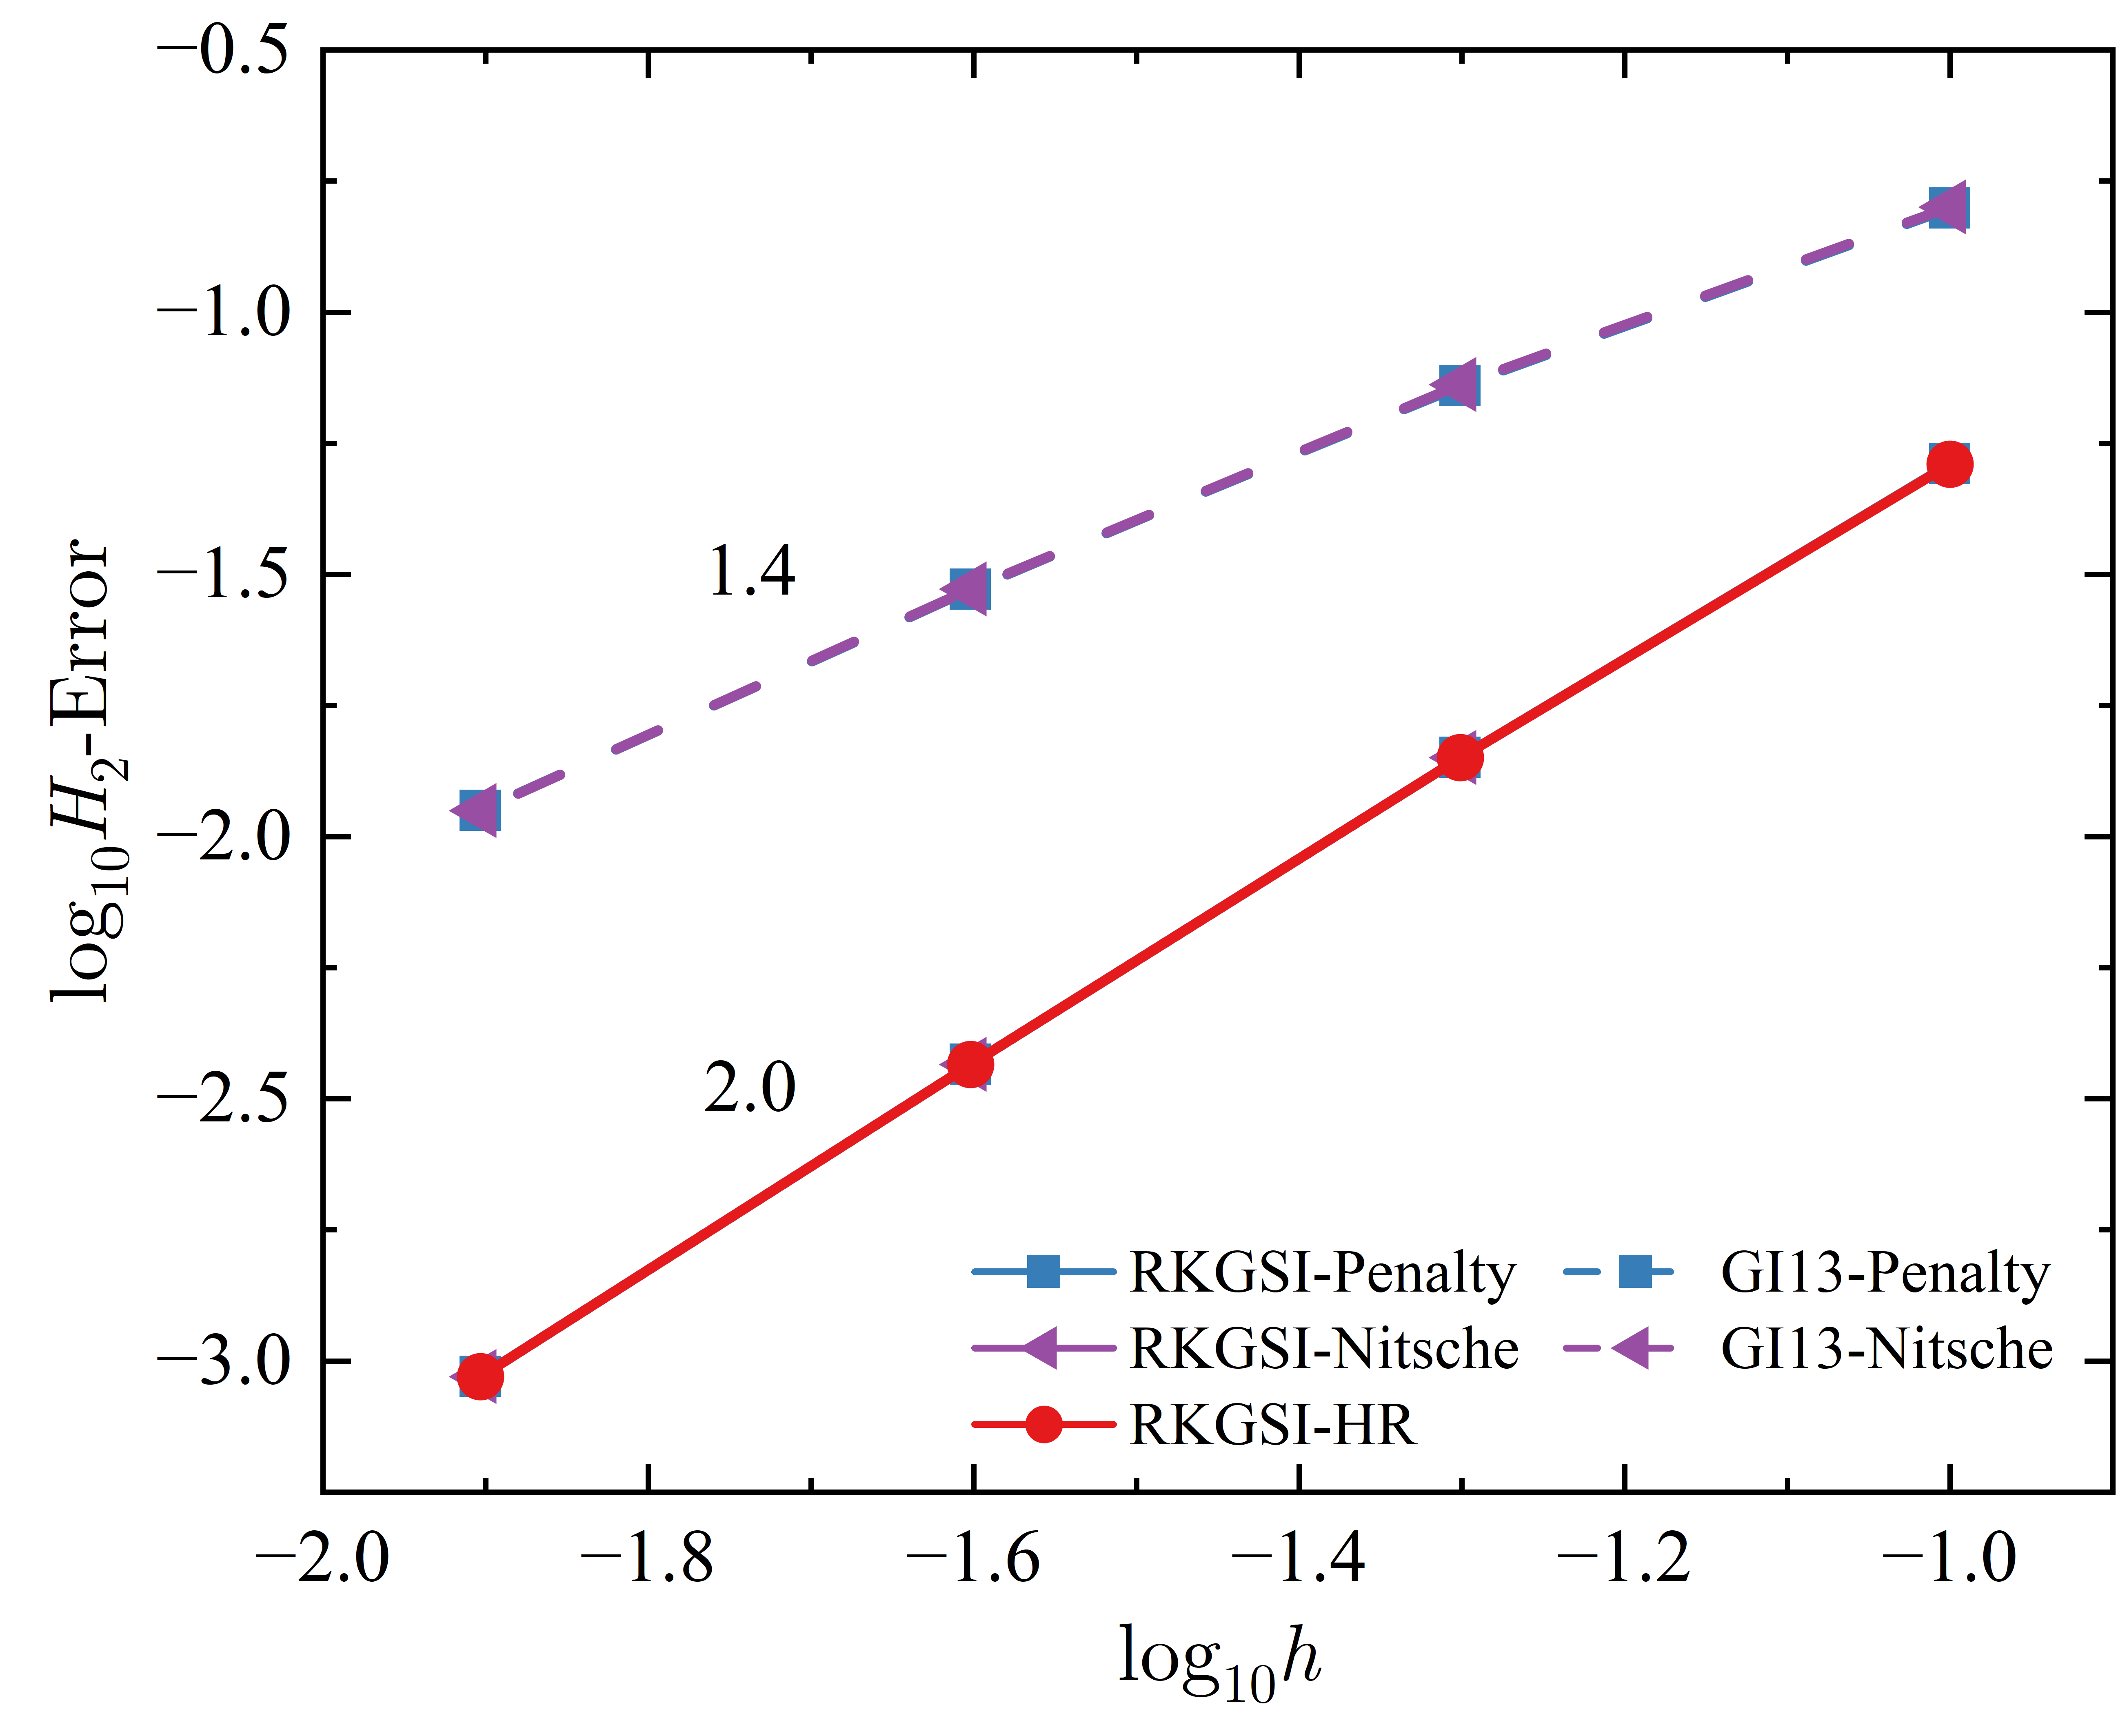
\includegraphics[width=0.49\textwidth]{figure/PHR/R/CH2.png}
    \phantomcaption\label{CH2}
    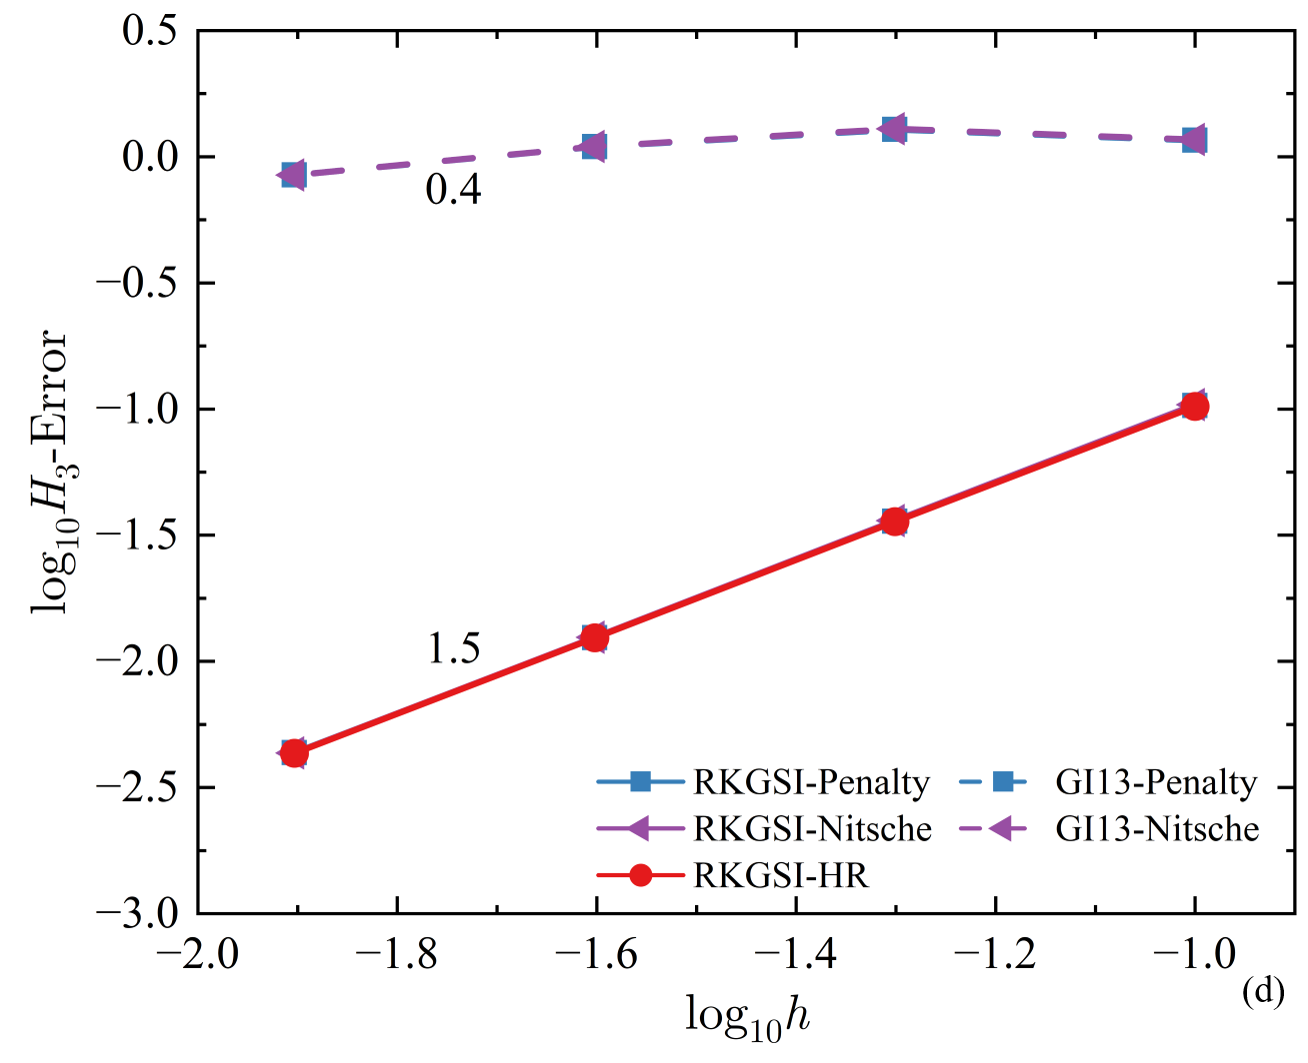
\includegraphics[width=0.49\textwidth]{figure/PHR/R/CH3.png}
    \phantomcaption\label{CH3}
    \end{subcaptiongroup}
\caption{简支方板问题三次基函数误差对比:\subref{CL2} $L_2$误差;\subref{CH1} $H_1$;误差\subref{CH2};$H_2$误差;\subref{CH3} $H_3$误差}
\label{RCLH}
\end{figure}
\newpage
\begin{figure}[H]
    \centering
    \begin{subcaptiongroup}
    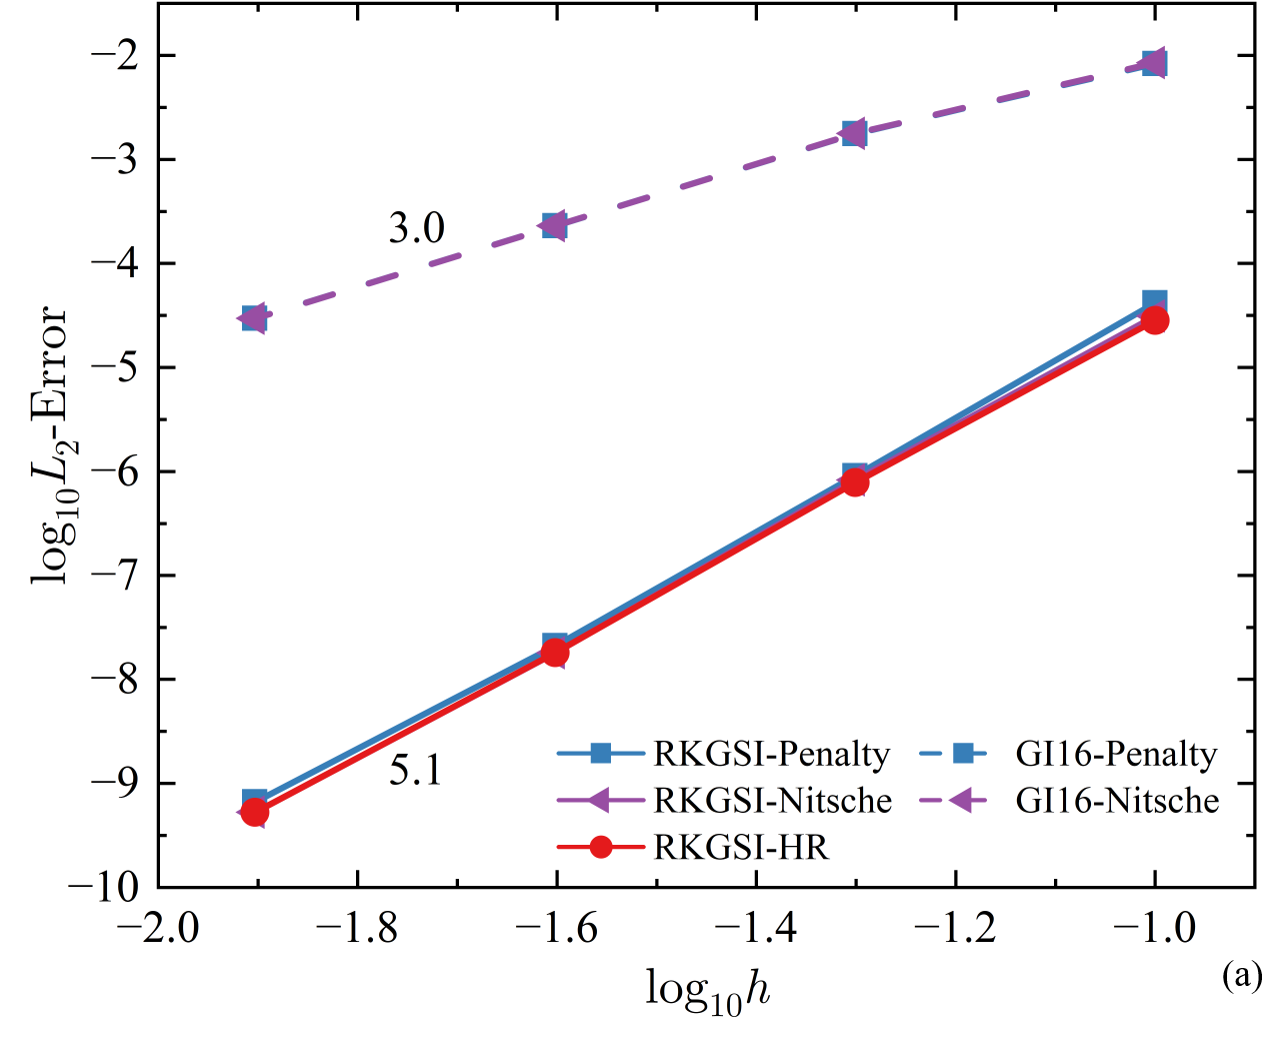
\includegraphics[width=0.49\textwidth]{figure/PHR/R/QL2.png}
    \phantomcaption\label{QL2}
    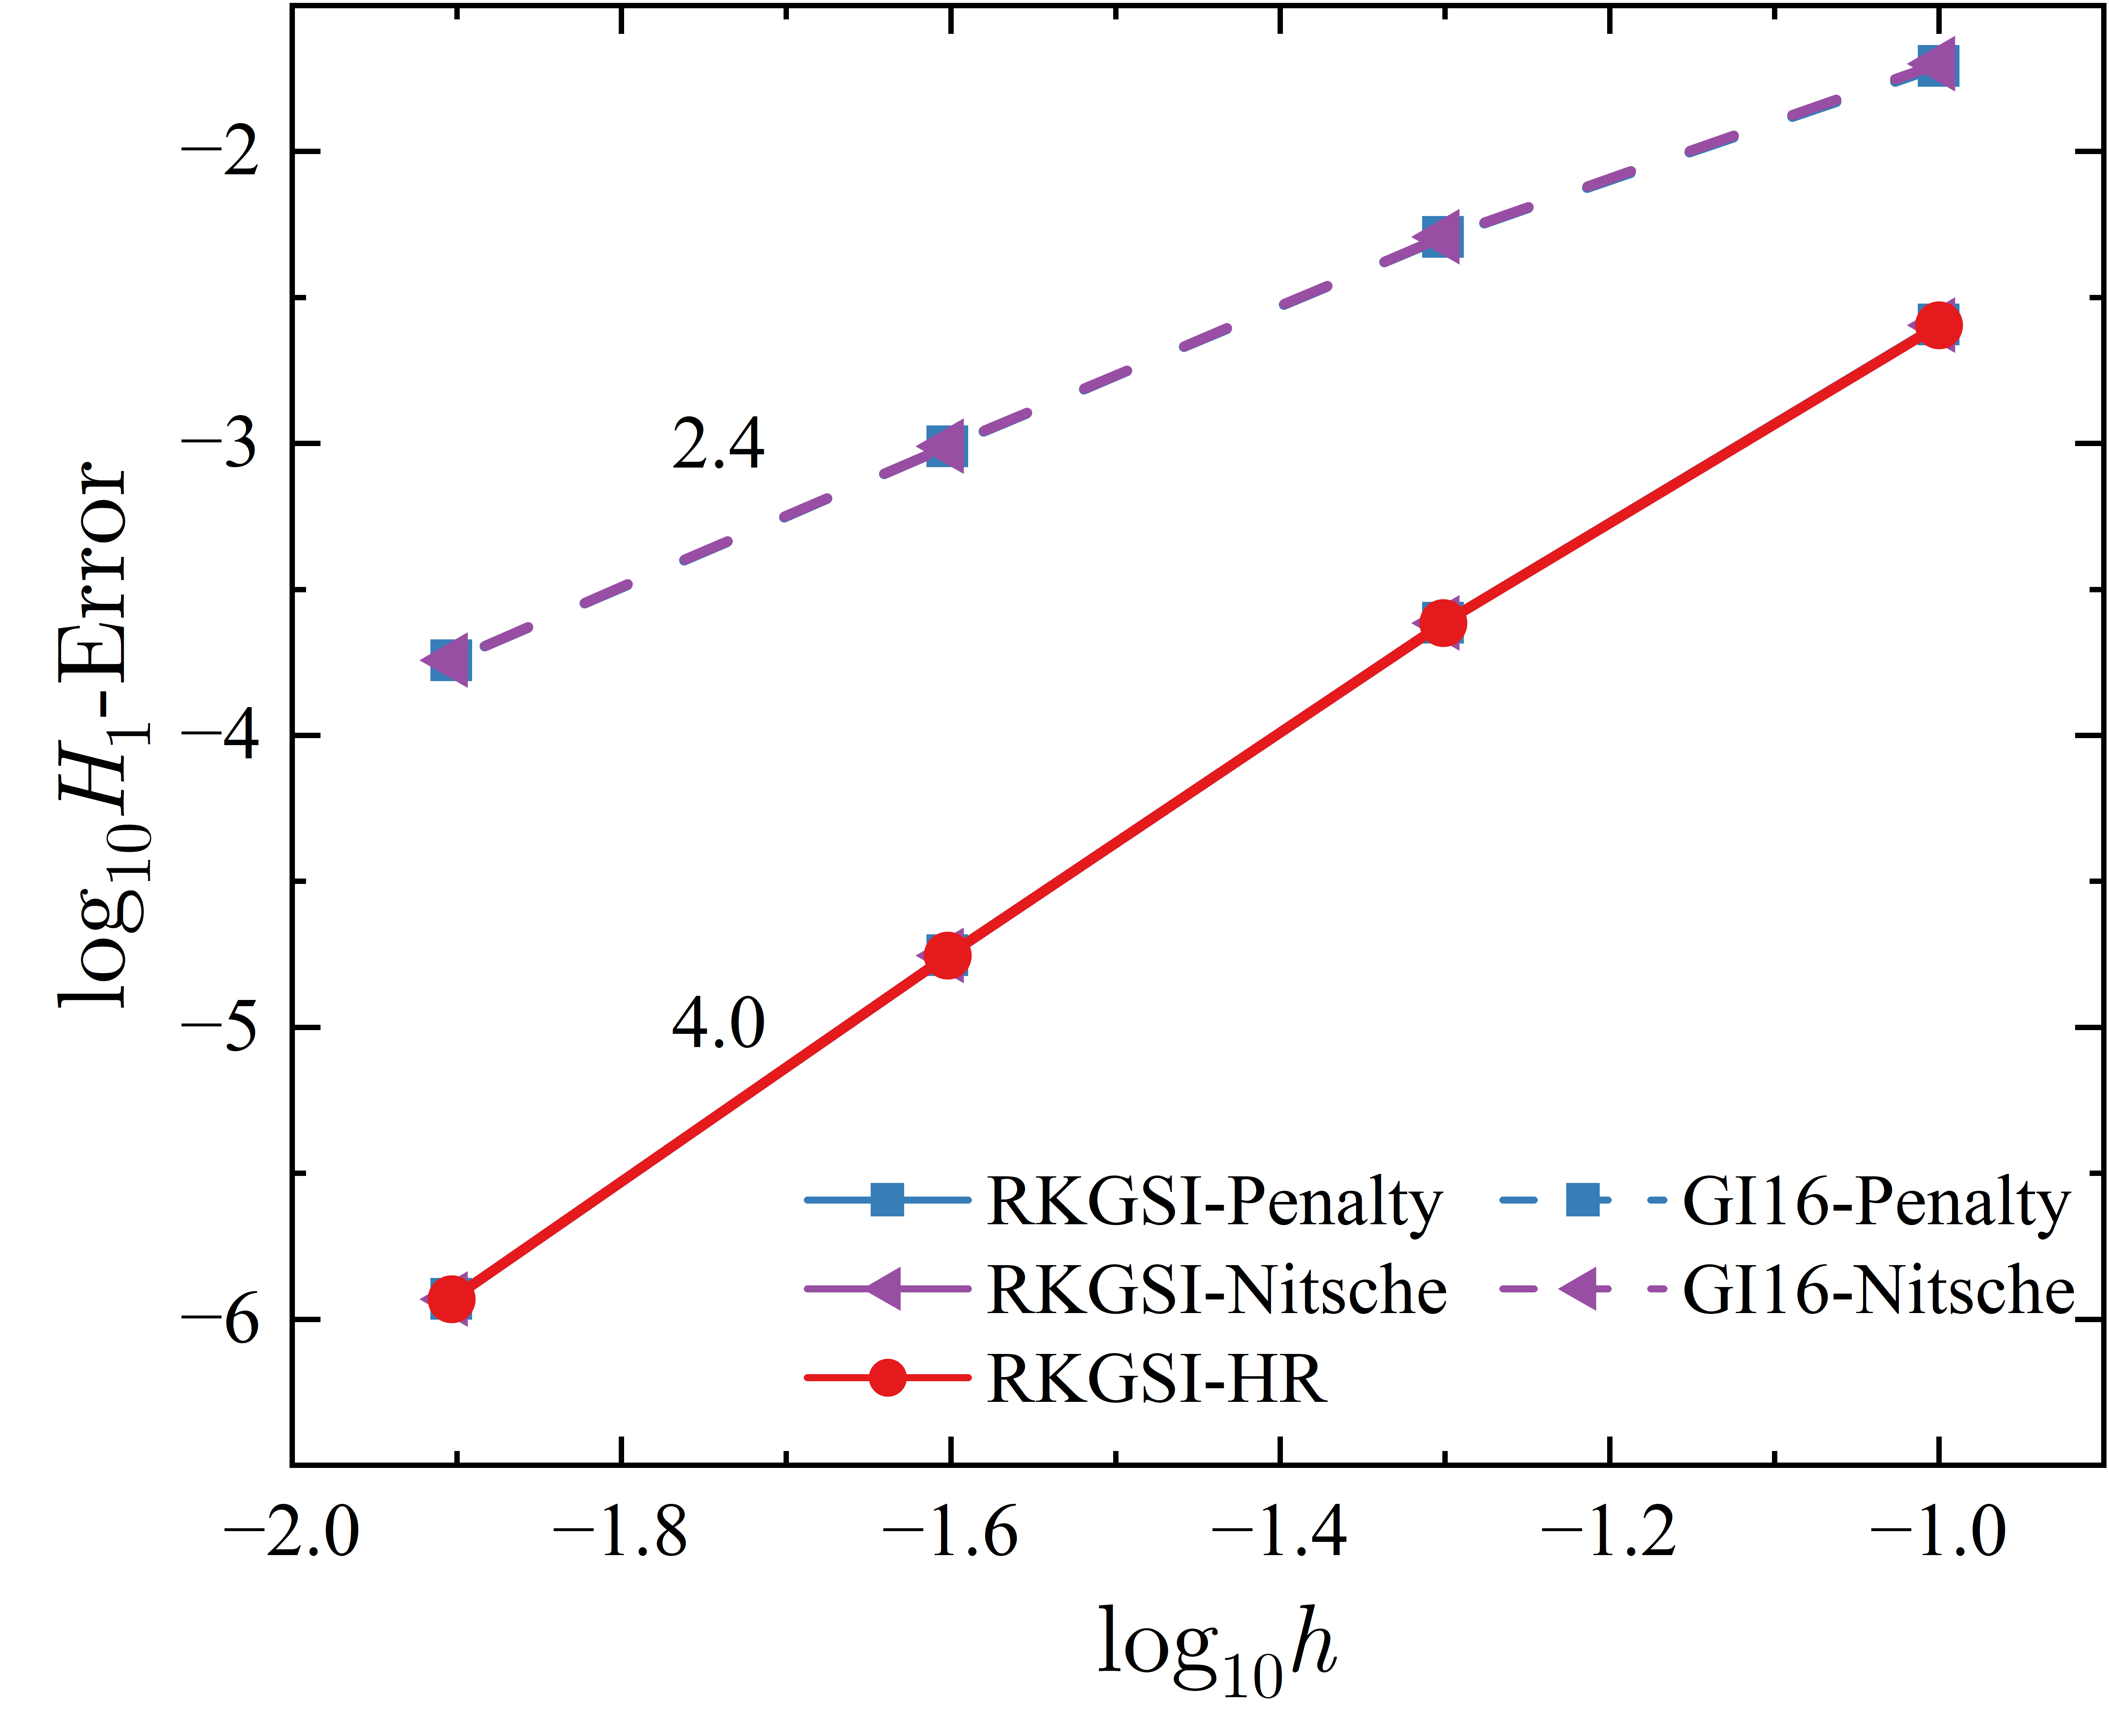
\includegraphics[width=0.49\textwidth]{figure/PHR/R/QH1.png}
    \phantomcaption\label{QH1}
    \label{dshape}
    \end{subcaptiongroup}
    \begin{subcaptiongroup}
    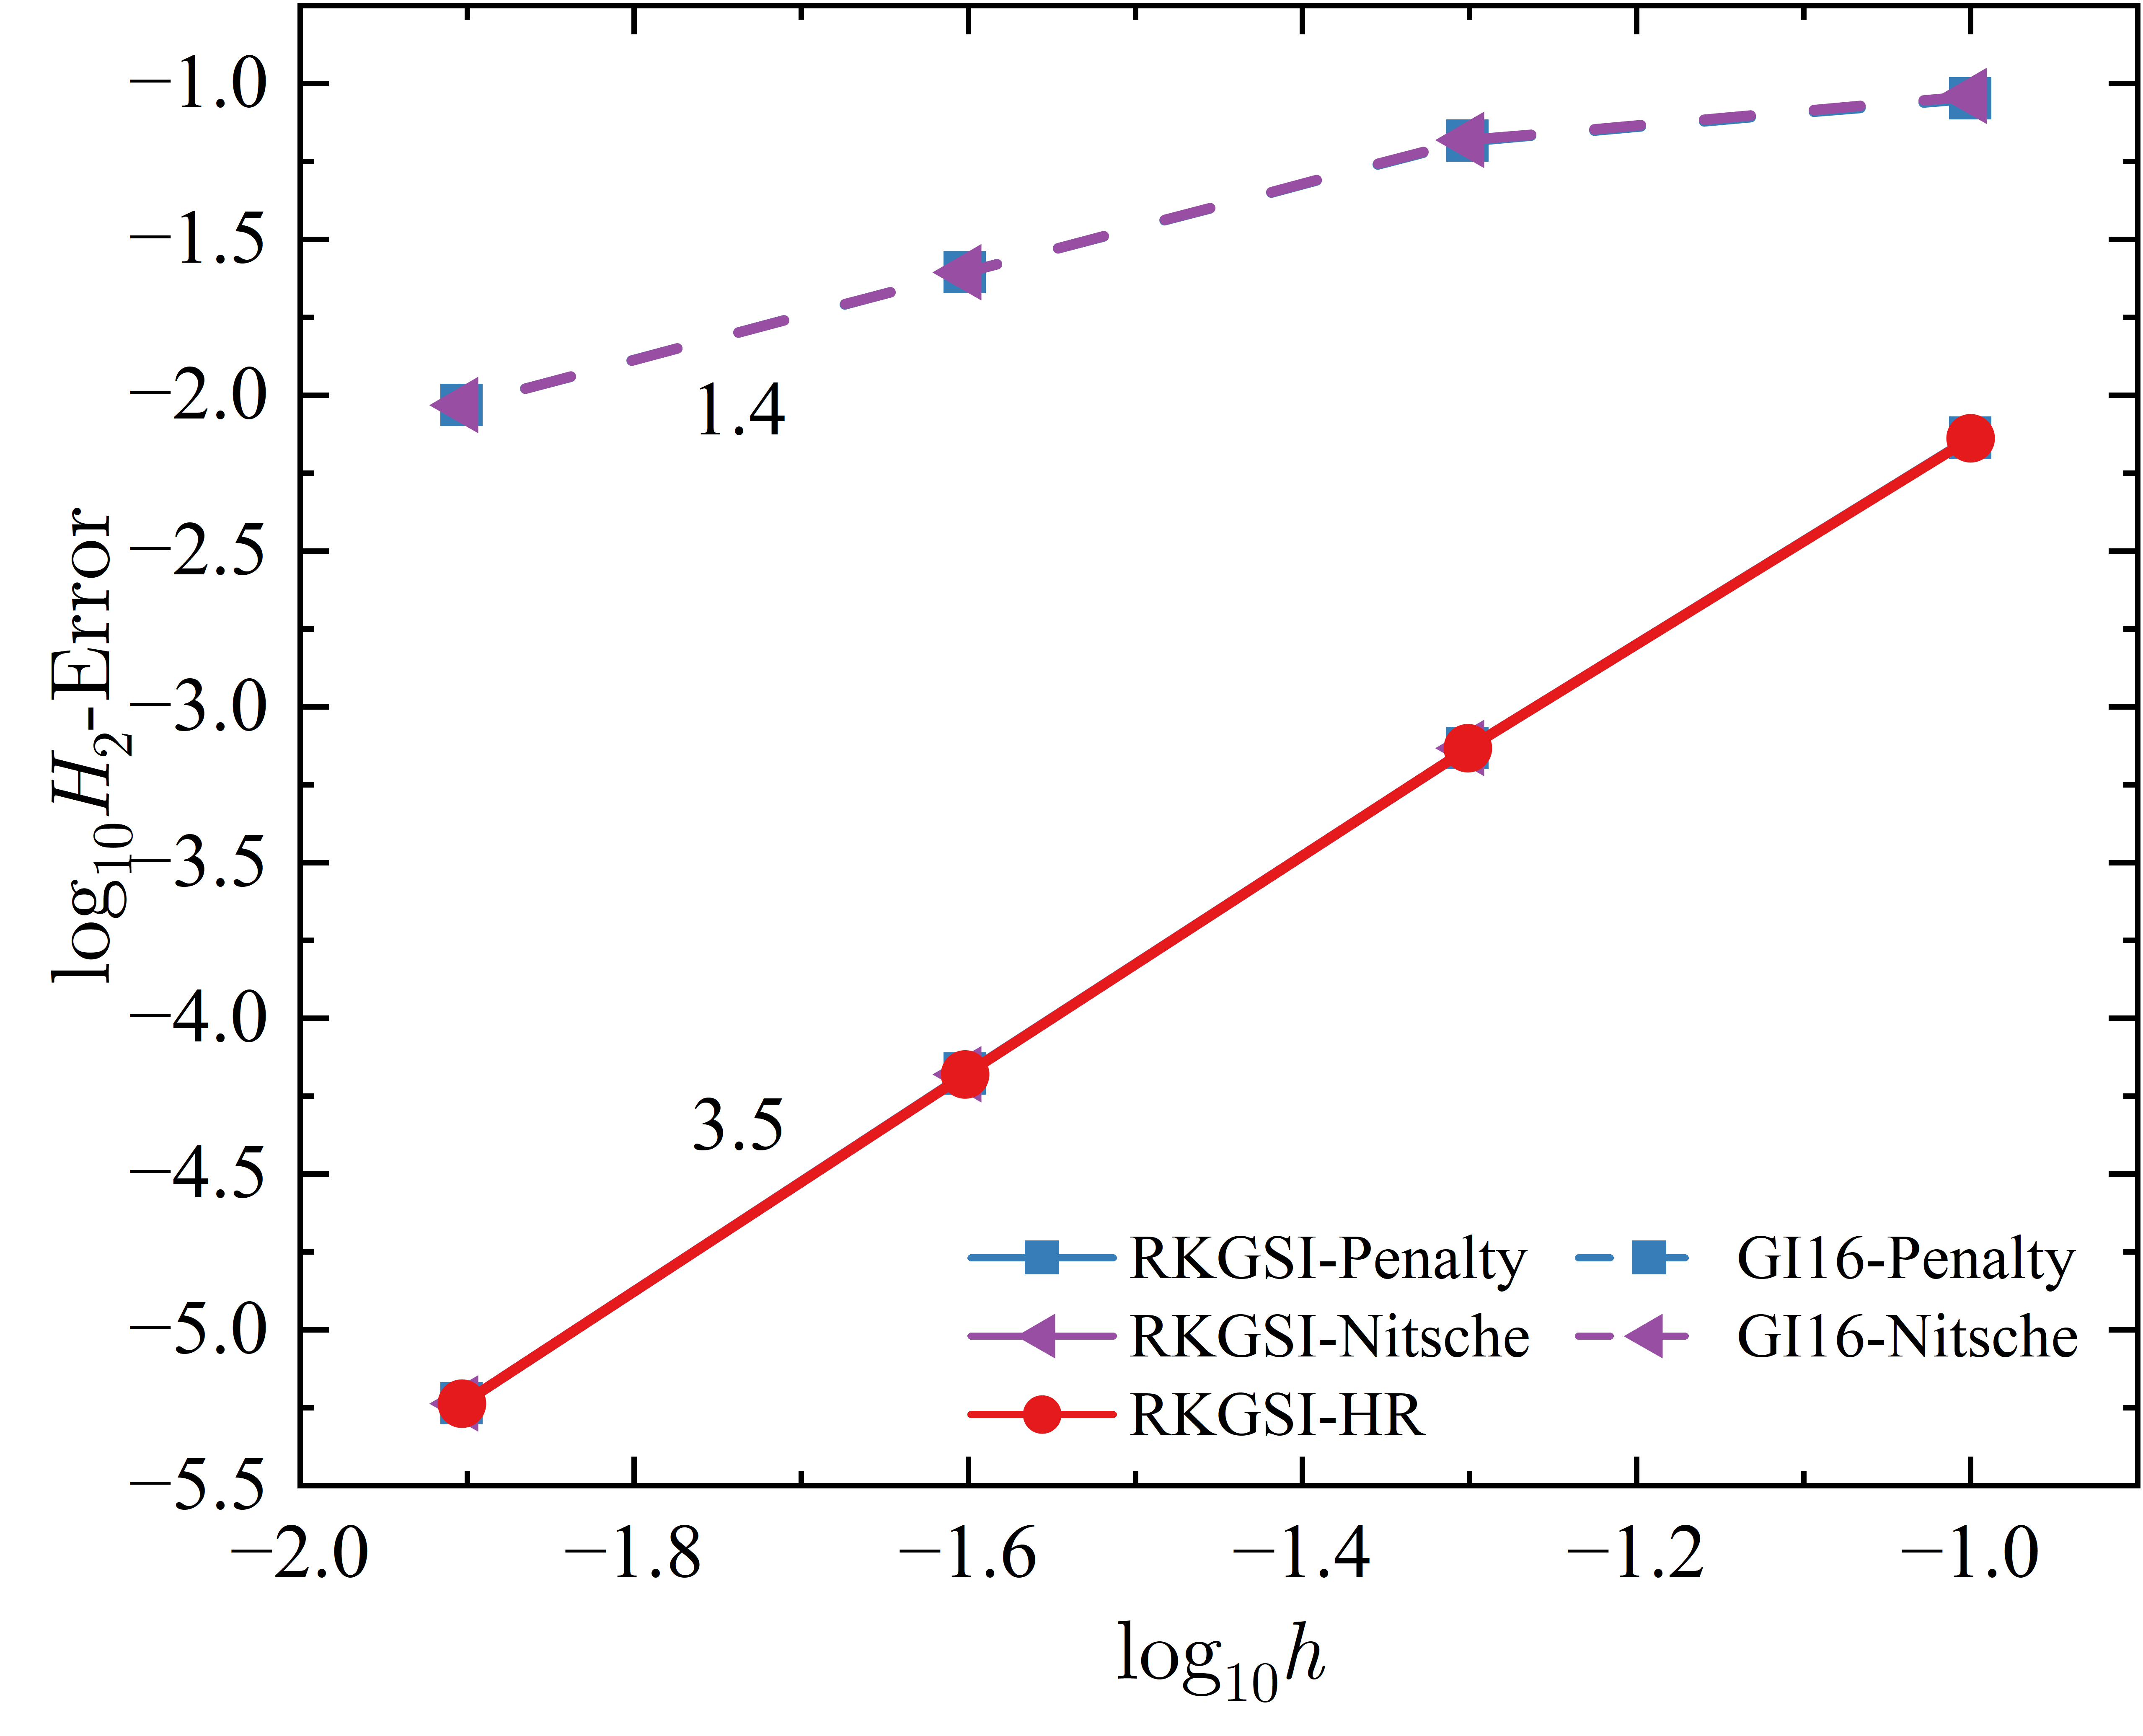
\includegraphics[width=0.49\textwidth]{figure/PHR/R/QH2.png}
    \phantomcaption\label{QH2}
    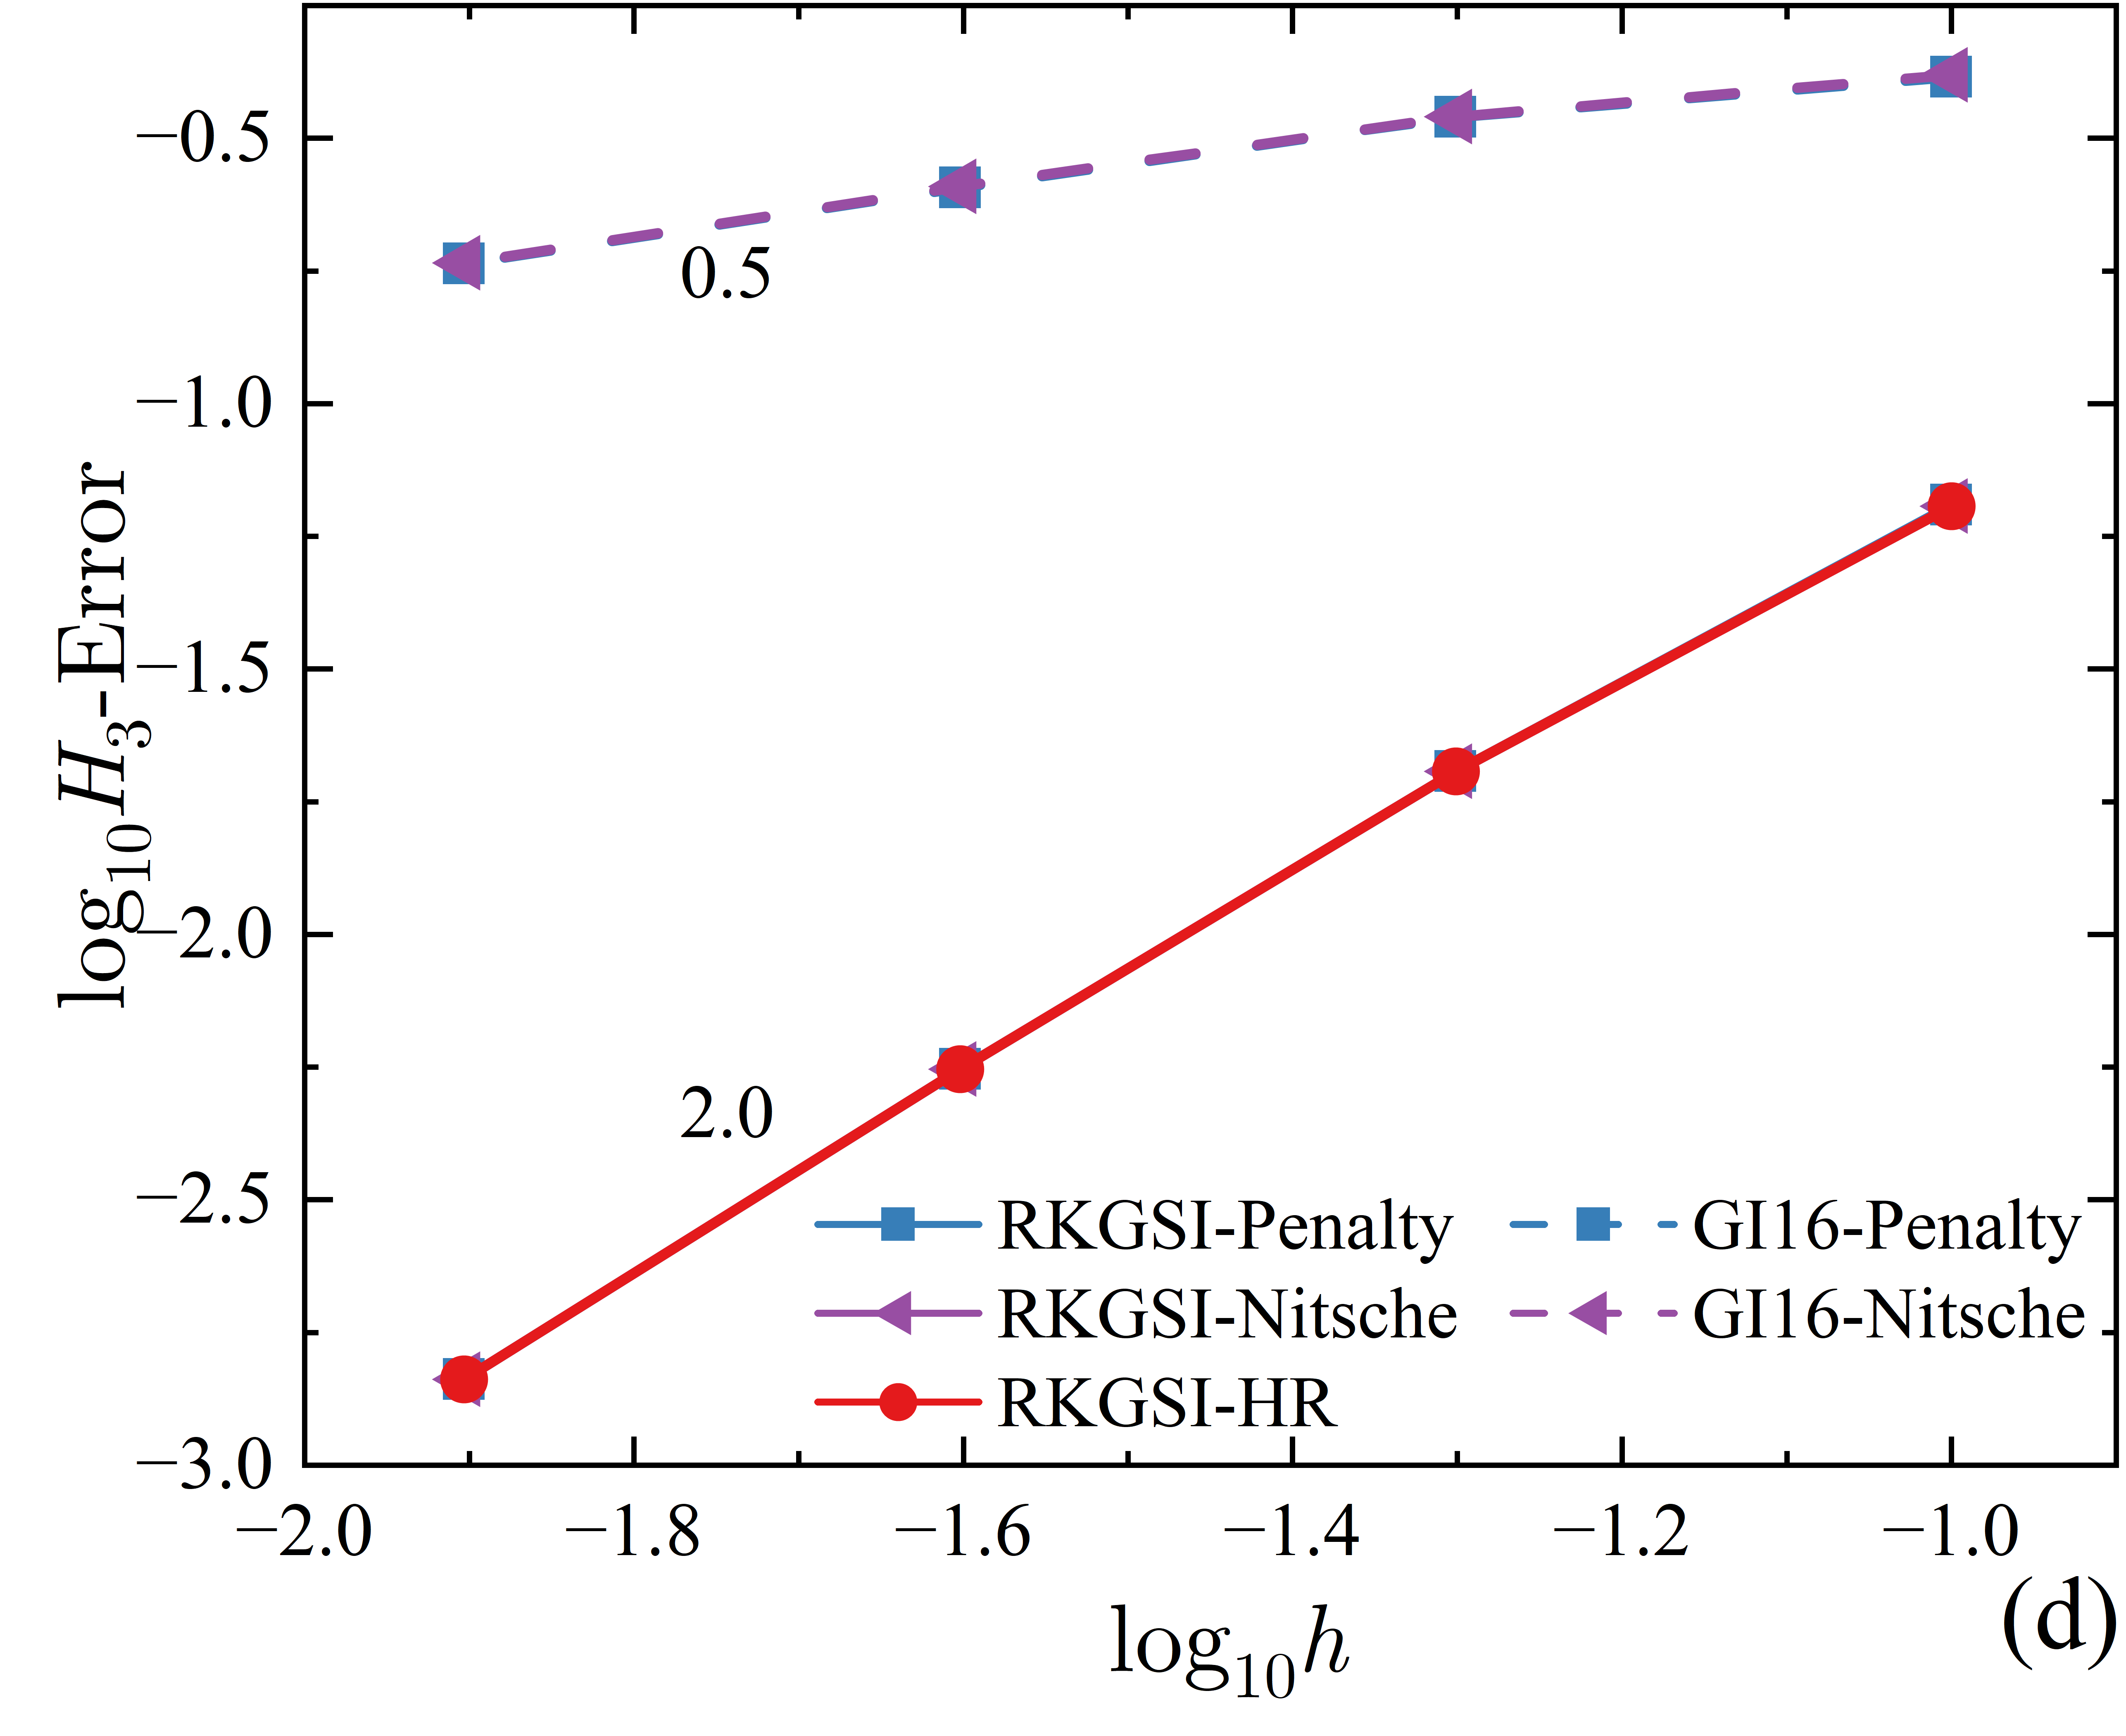
\includegraphics[width=0.49\textwidth]{figure/PHR/R/QH3.png}
    \phantomcaption\label{QH3}
    \label{dshape}
    \end{subcaptiongroup}
\caption{简支方板问题四次基函数误差对比:\subref{QL2} $L_2$误差;\subref{QH1} $H_1$误差;\subref{QH2};$H_2$误差;\subref{QH3} $H_3$误差}
\label{RQLH}
\end{figure}
\begin{figure}[H]
    \centering
    \begin{subcaptiongroup}
    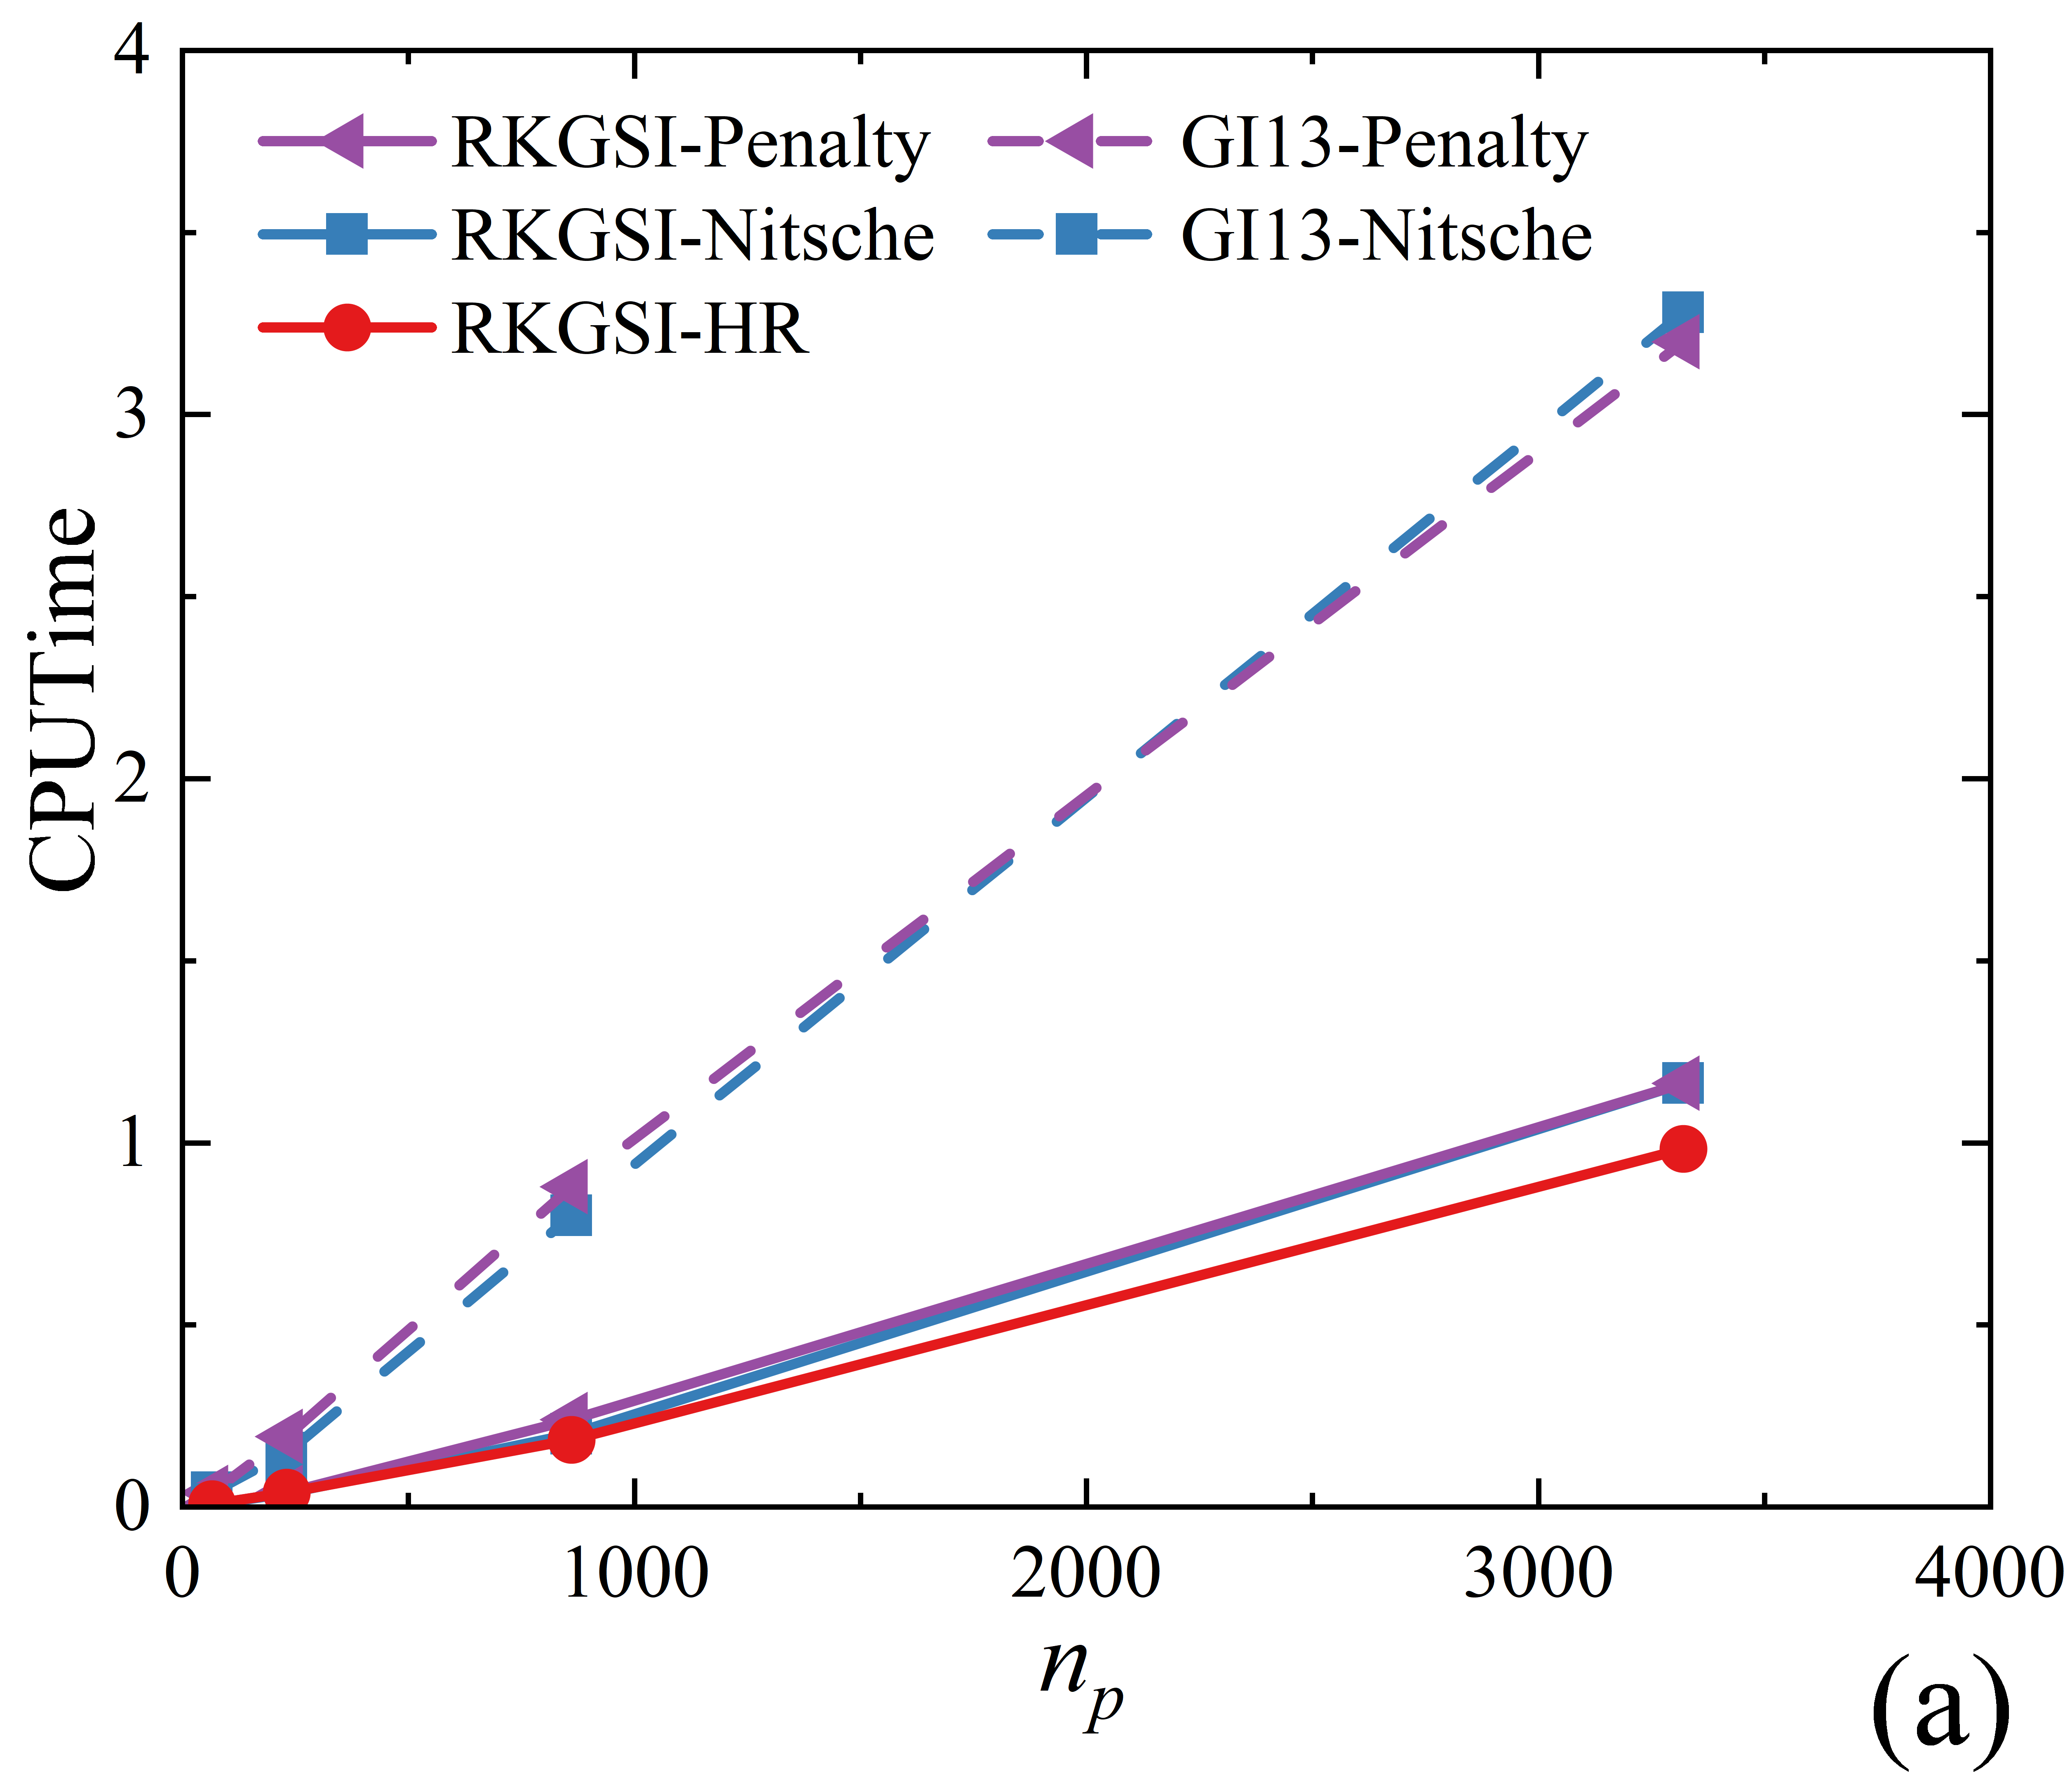
\includegraphics[width=0.49\textwidth]{figure/PHR/R/Ccputime.png}
    \phantomcaption\label{Ccputime}
    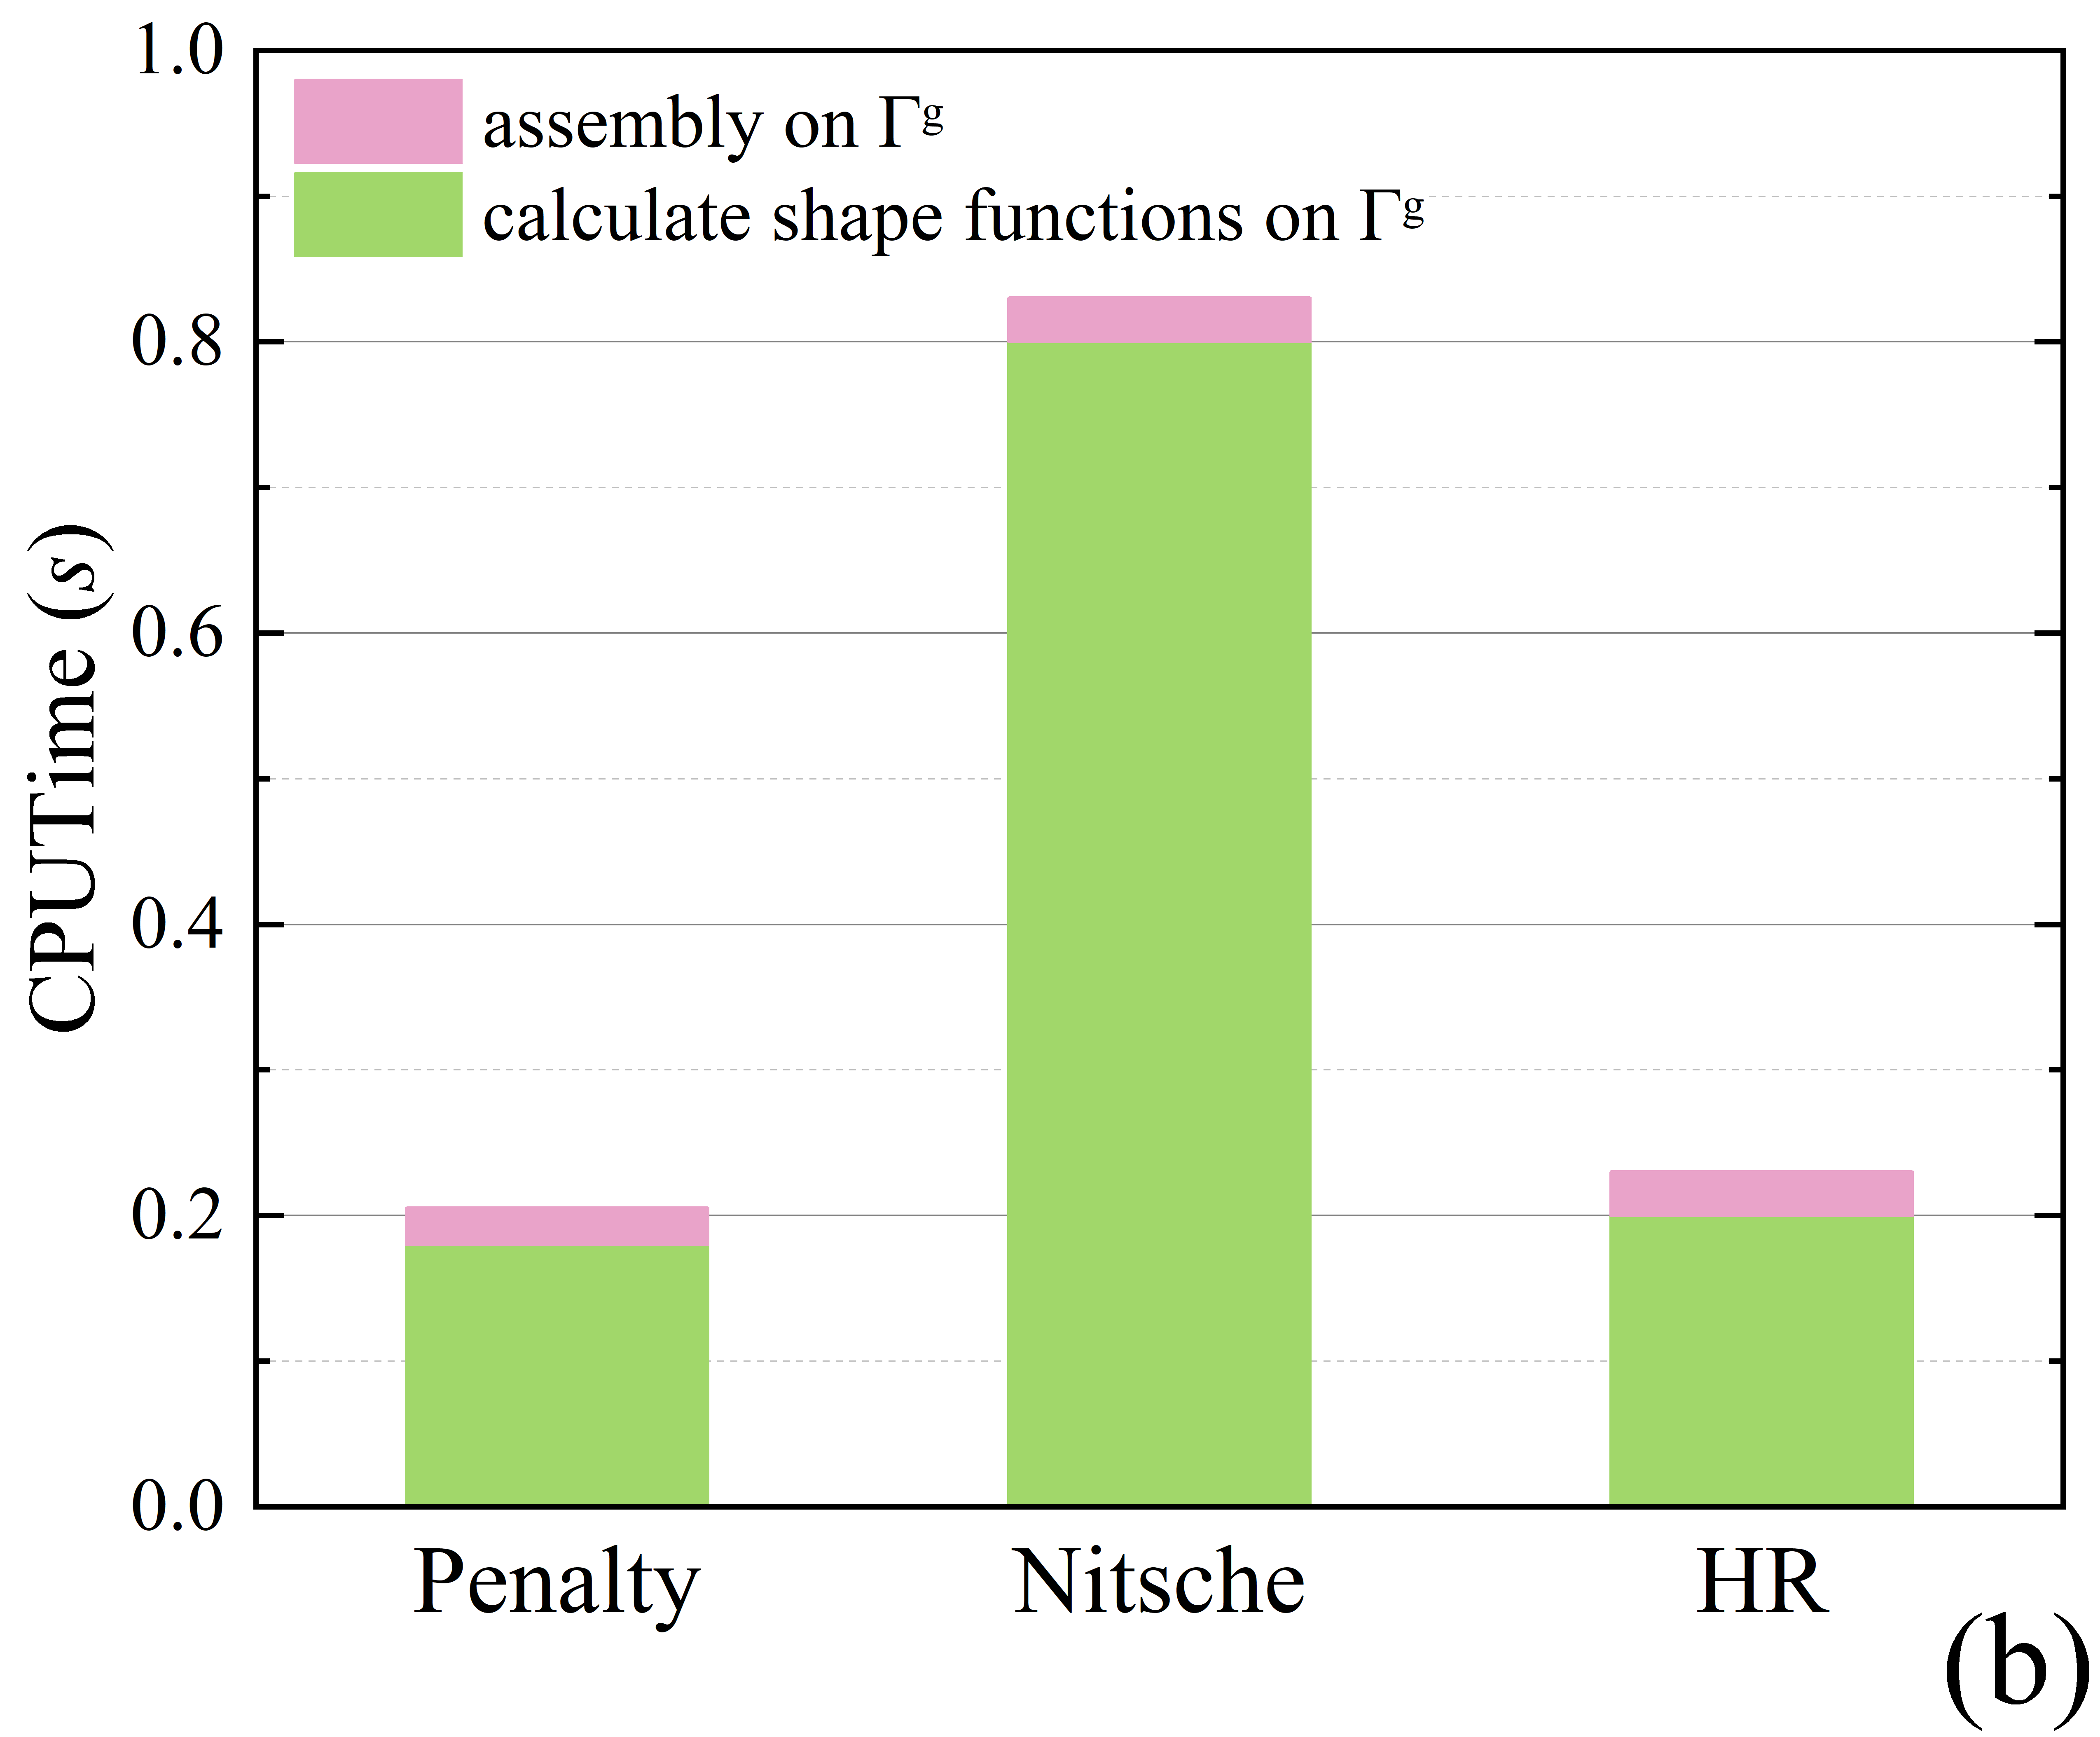
\includegraphics[width=0.49\textwidth]{figure/PHR/R/Cefficiency.png}
    \phantomcaption\label{Cefficiency}
    \end{subcaptiongroup}
\caption{简支方板问题三次基函数效率对比:\subref{Ccputime}计算时间与节点数的关系;\subref{Cefficiency}本质边界条件施加效率分析}
\label{RCcputime}
\end{figure}
\newpage
\begin{figure}[H]
    \centering
    \begin{subcaptiongroup}
    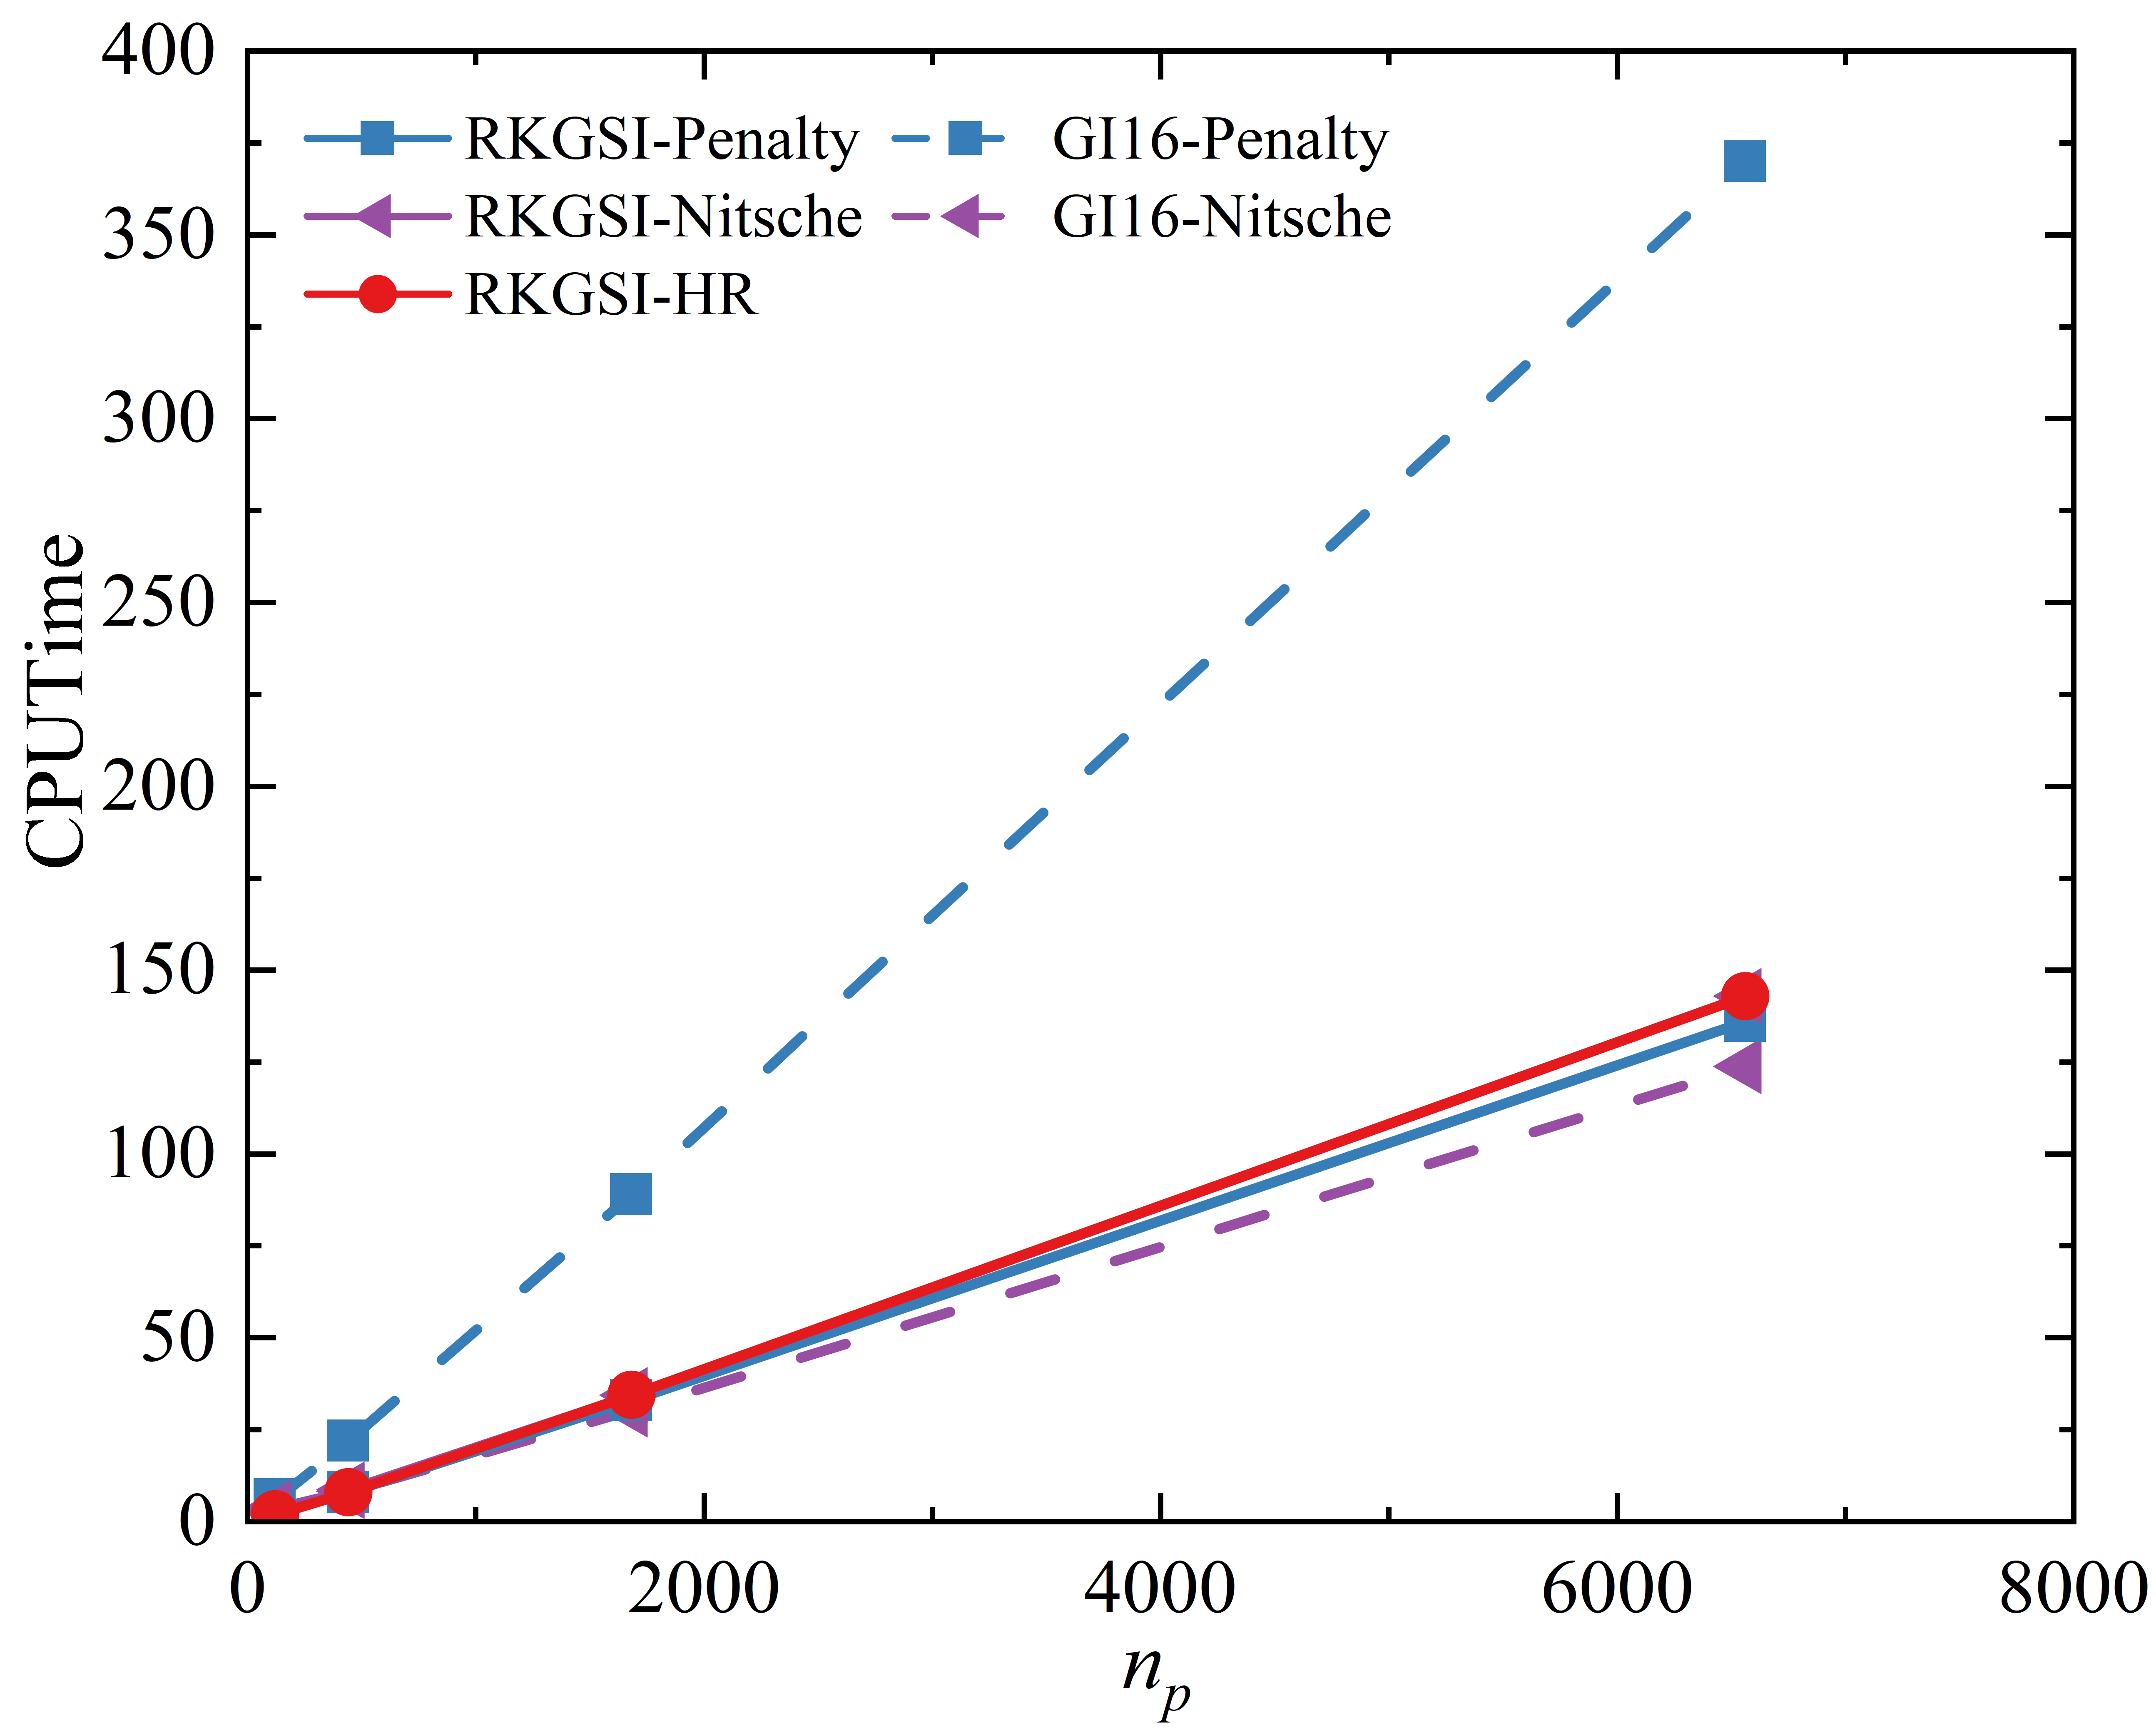
\includegraphics[width=0.49\textwidth]{figure/PHR/R/Qcputime.png}
    \phantomcaption\label{Qcputime}
    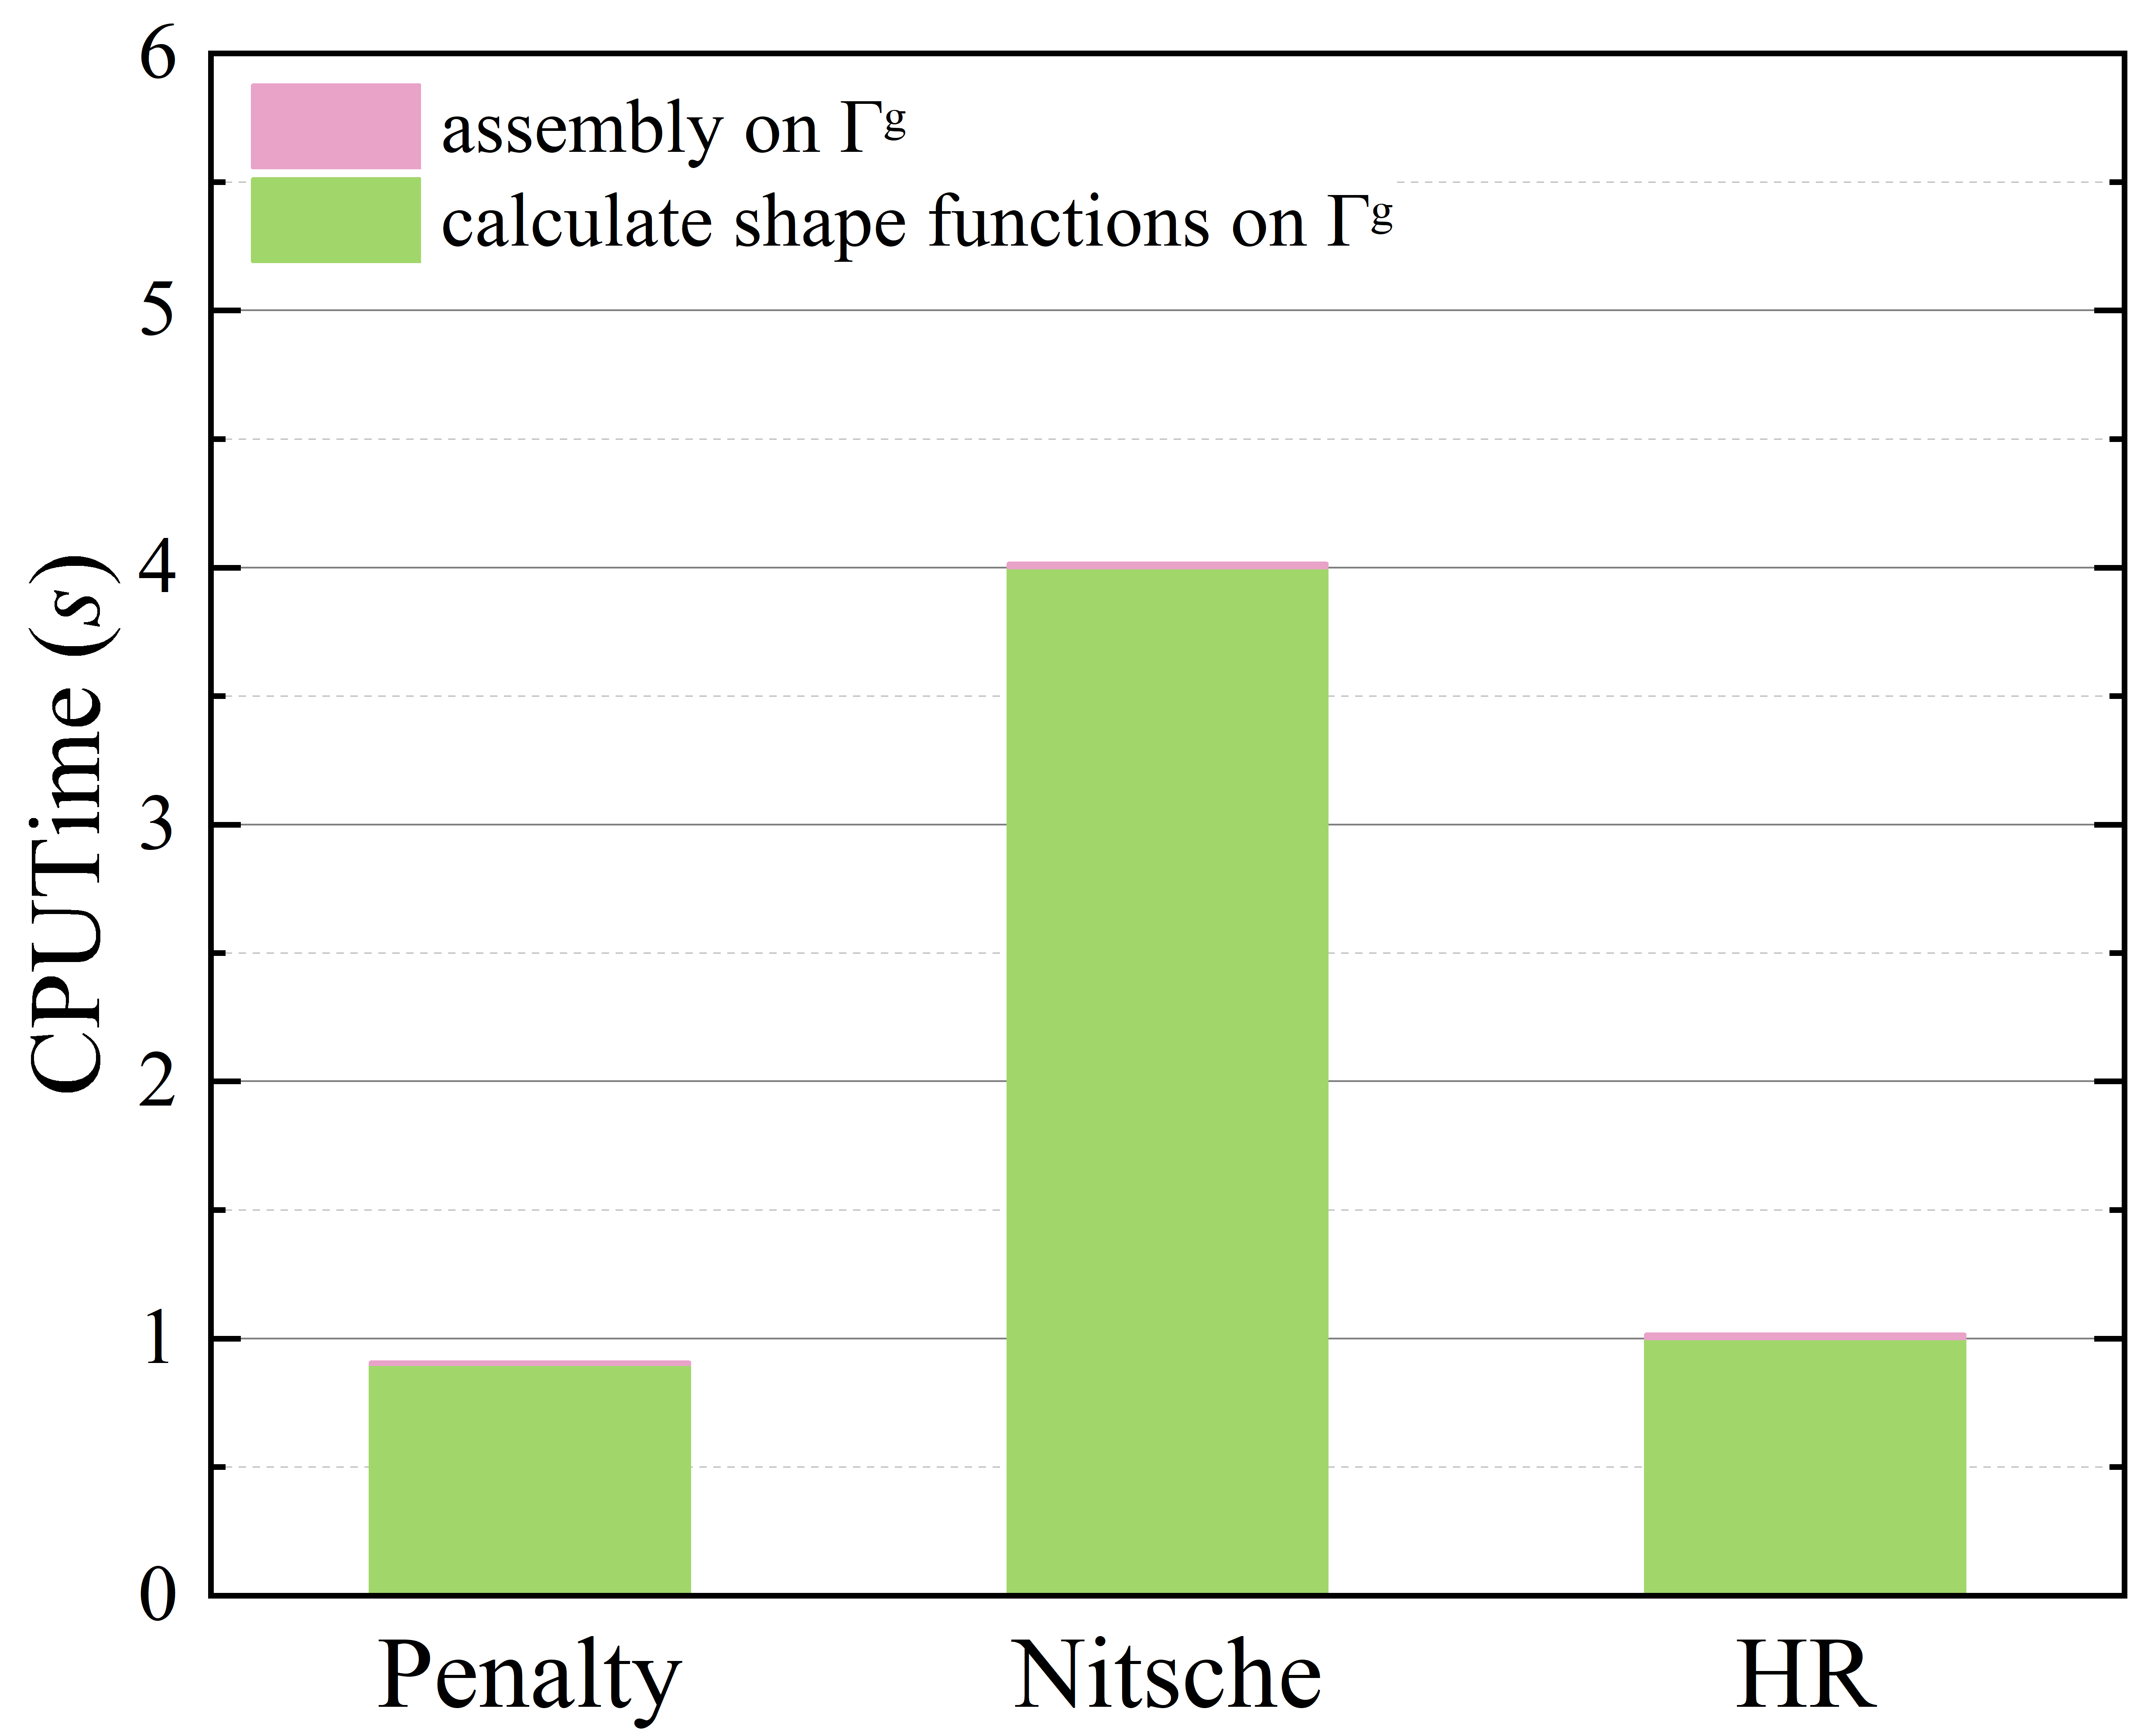
\includegraphics[width=0.49\textwidth]{figure/PHR/R/Qefficiency.png}
    \phantomcaption\label{Qefficiency}
    \end{subcaptiongroup}
\caption{简支方板问题四次基函数效率对比:\subref{Qcputime}计算时间与节点数的关系;\subref{Cefficiency}本质边界条件施加效率分析}
\label{RQcputime}
\end{figure}
图(\ref{Ralpha})是分别验证简支方板问题在三次基函数和四次基函数时带有人工经验参数的罚函数法和Nitsche法的敏感度分析。
从图中可以明显的看出,不同的经验参数对罚函数法的误差有着很大的影响,并且它的最优误差只在一小部分。
Nitsche法的最优误差的人工经验参数的范围比较大,但人工经验参数值的大小仍然会影响误差结果的变化,
并且随着网格的加密,人工经验参数的最优结果是在发生改变的。此时,提出的基于Hellinger-Reissner变分原理
中由于内嵌了本质边界条件,无需人工经验参数来满足正定性,相较于同样满足积分约束条件的“RKGSI-Nitsche”法,提出的“RKGSI-HR”法的不因人工参数值的变化影响最优误差。
\begin{figure}[H]
    \centering
    \begin{subcaptiongroup}
    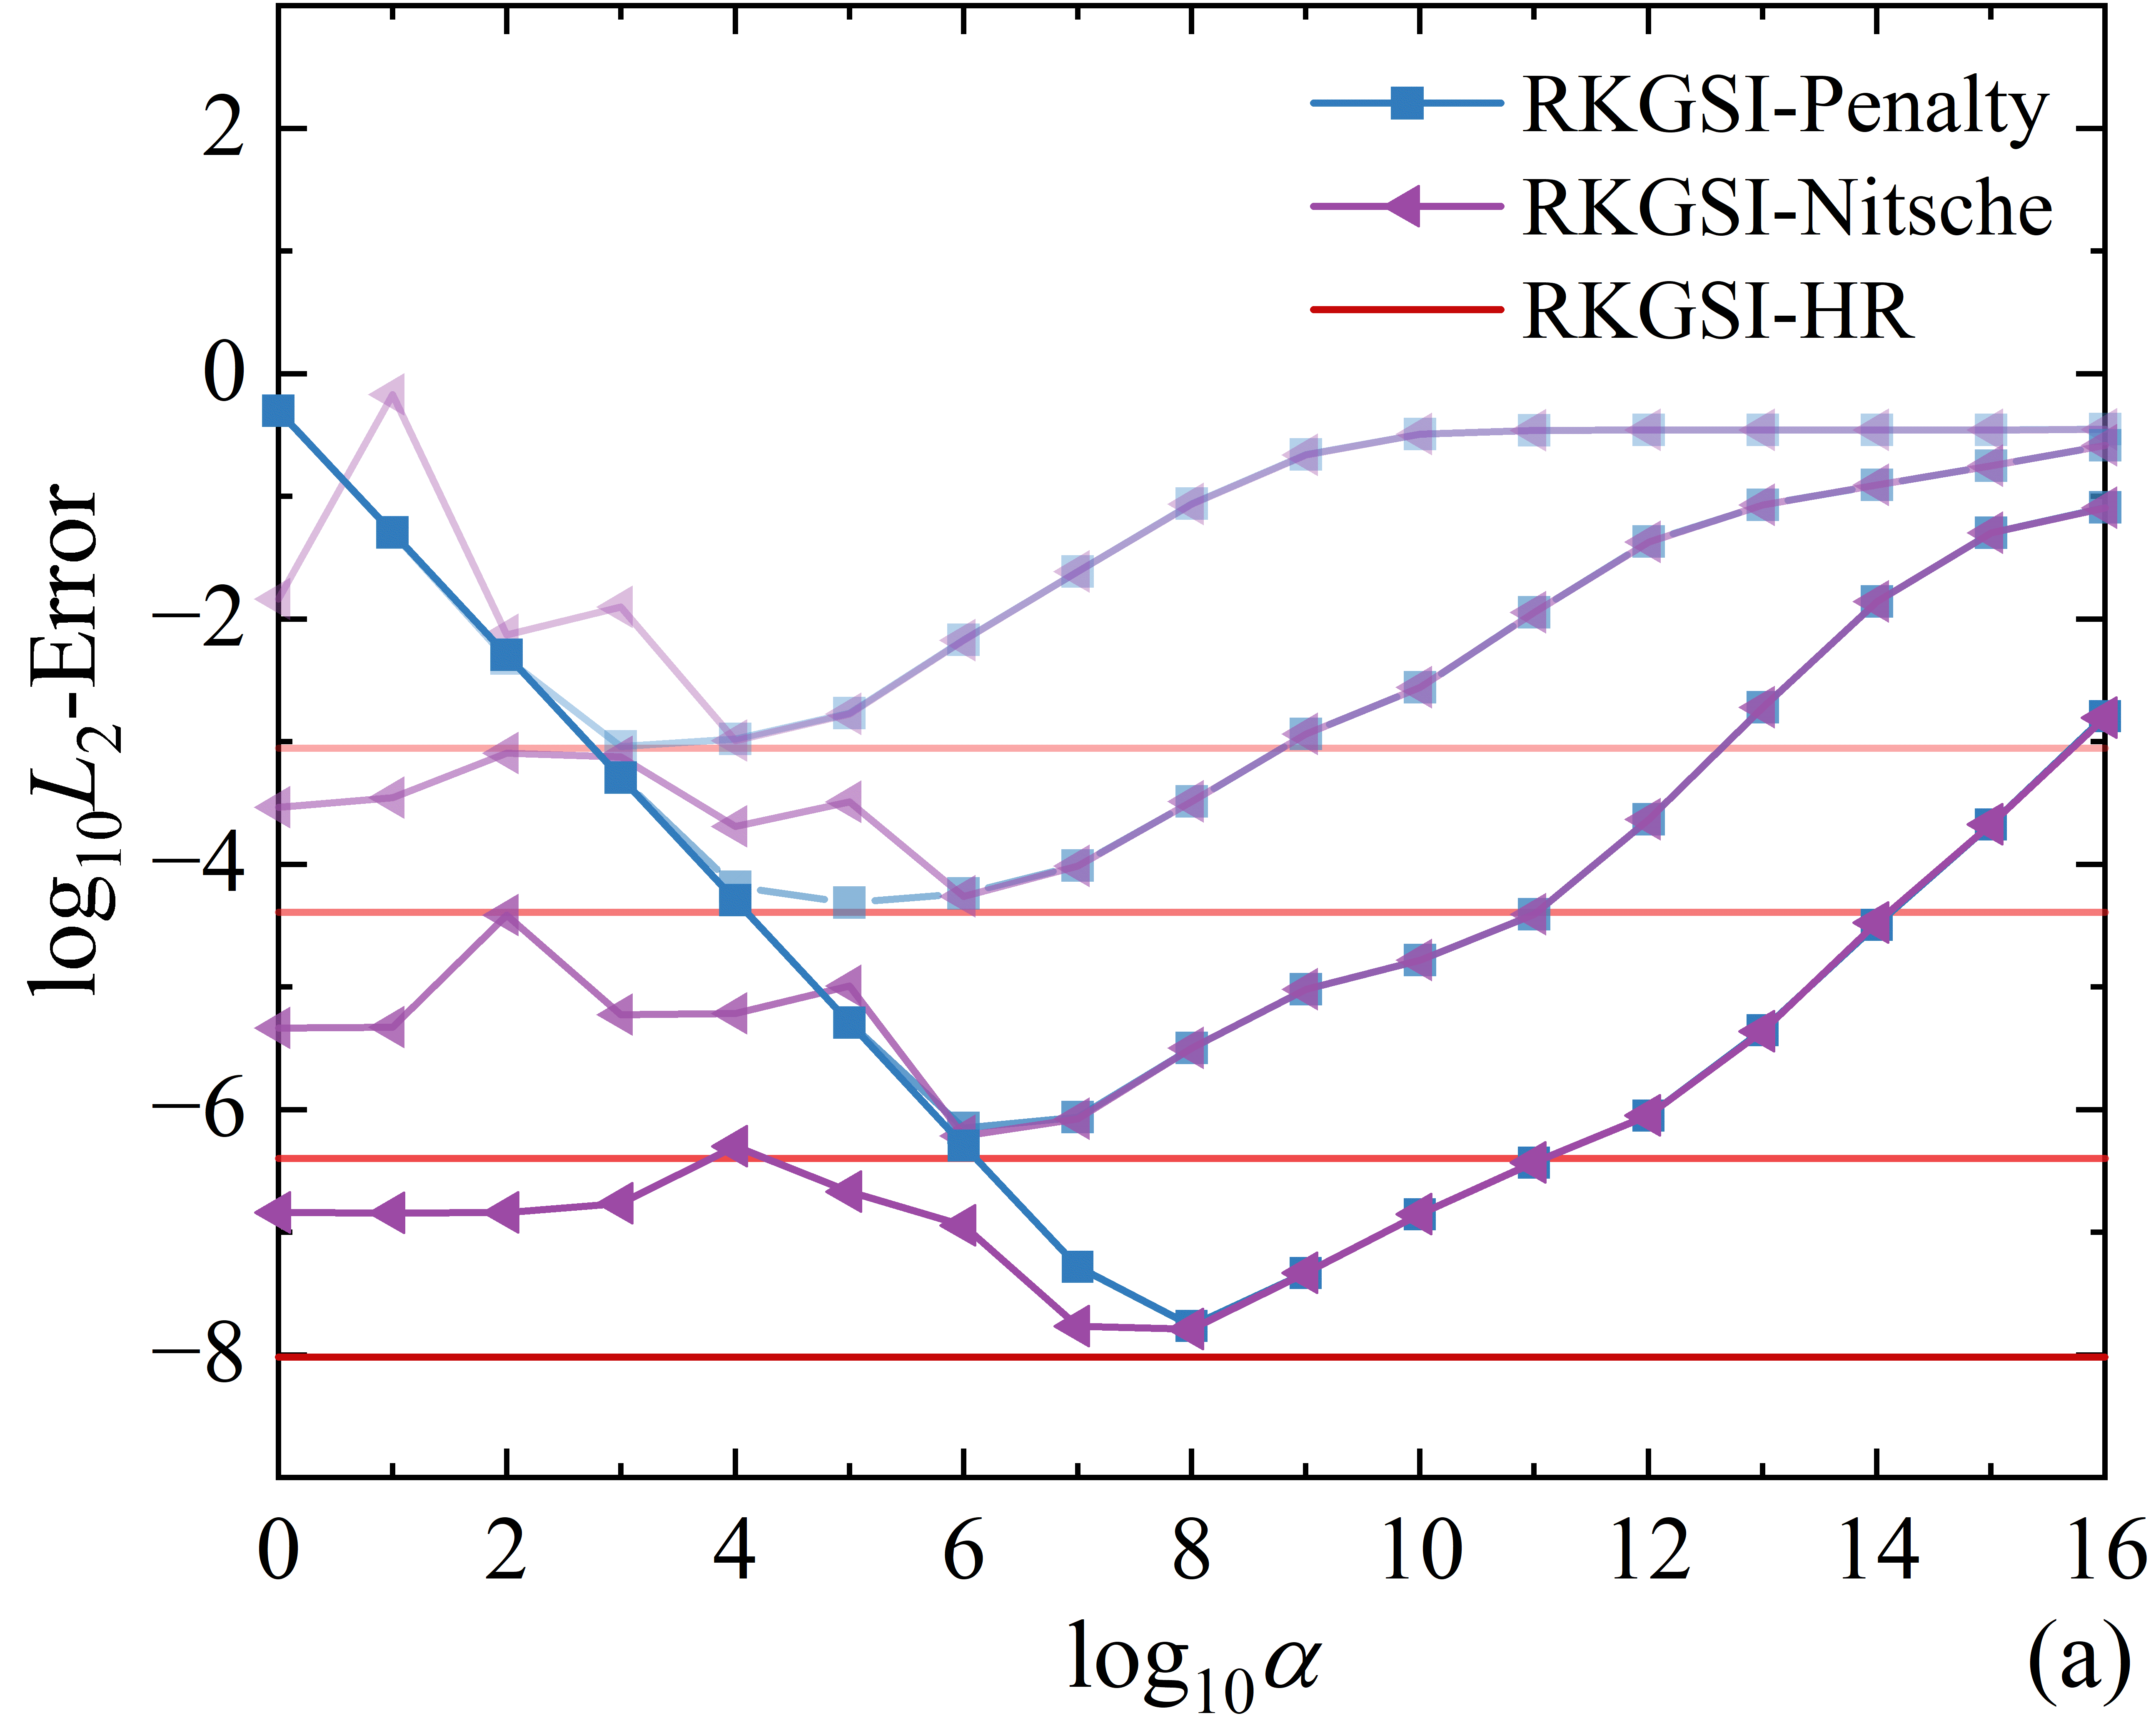
\includegraphics[width=0.49\textwidth]{figure/PHR/R/calpha.png}
    \phantomcaption\label{calpha}
    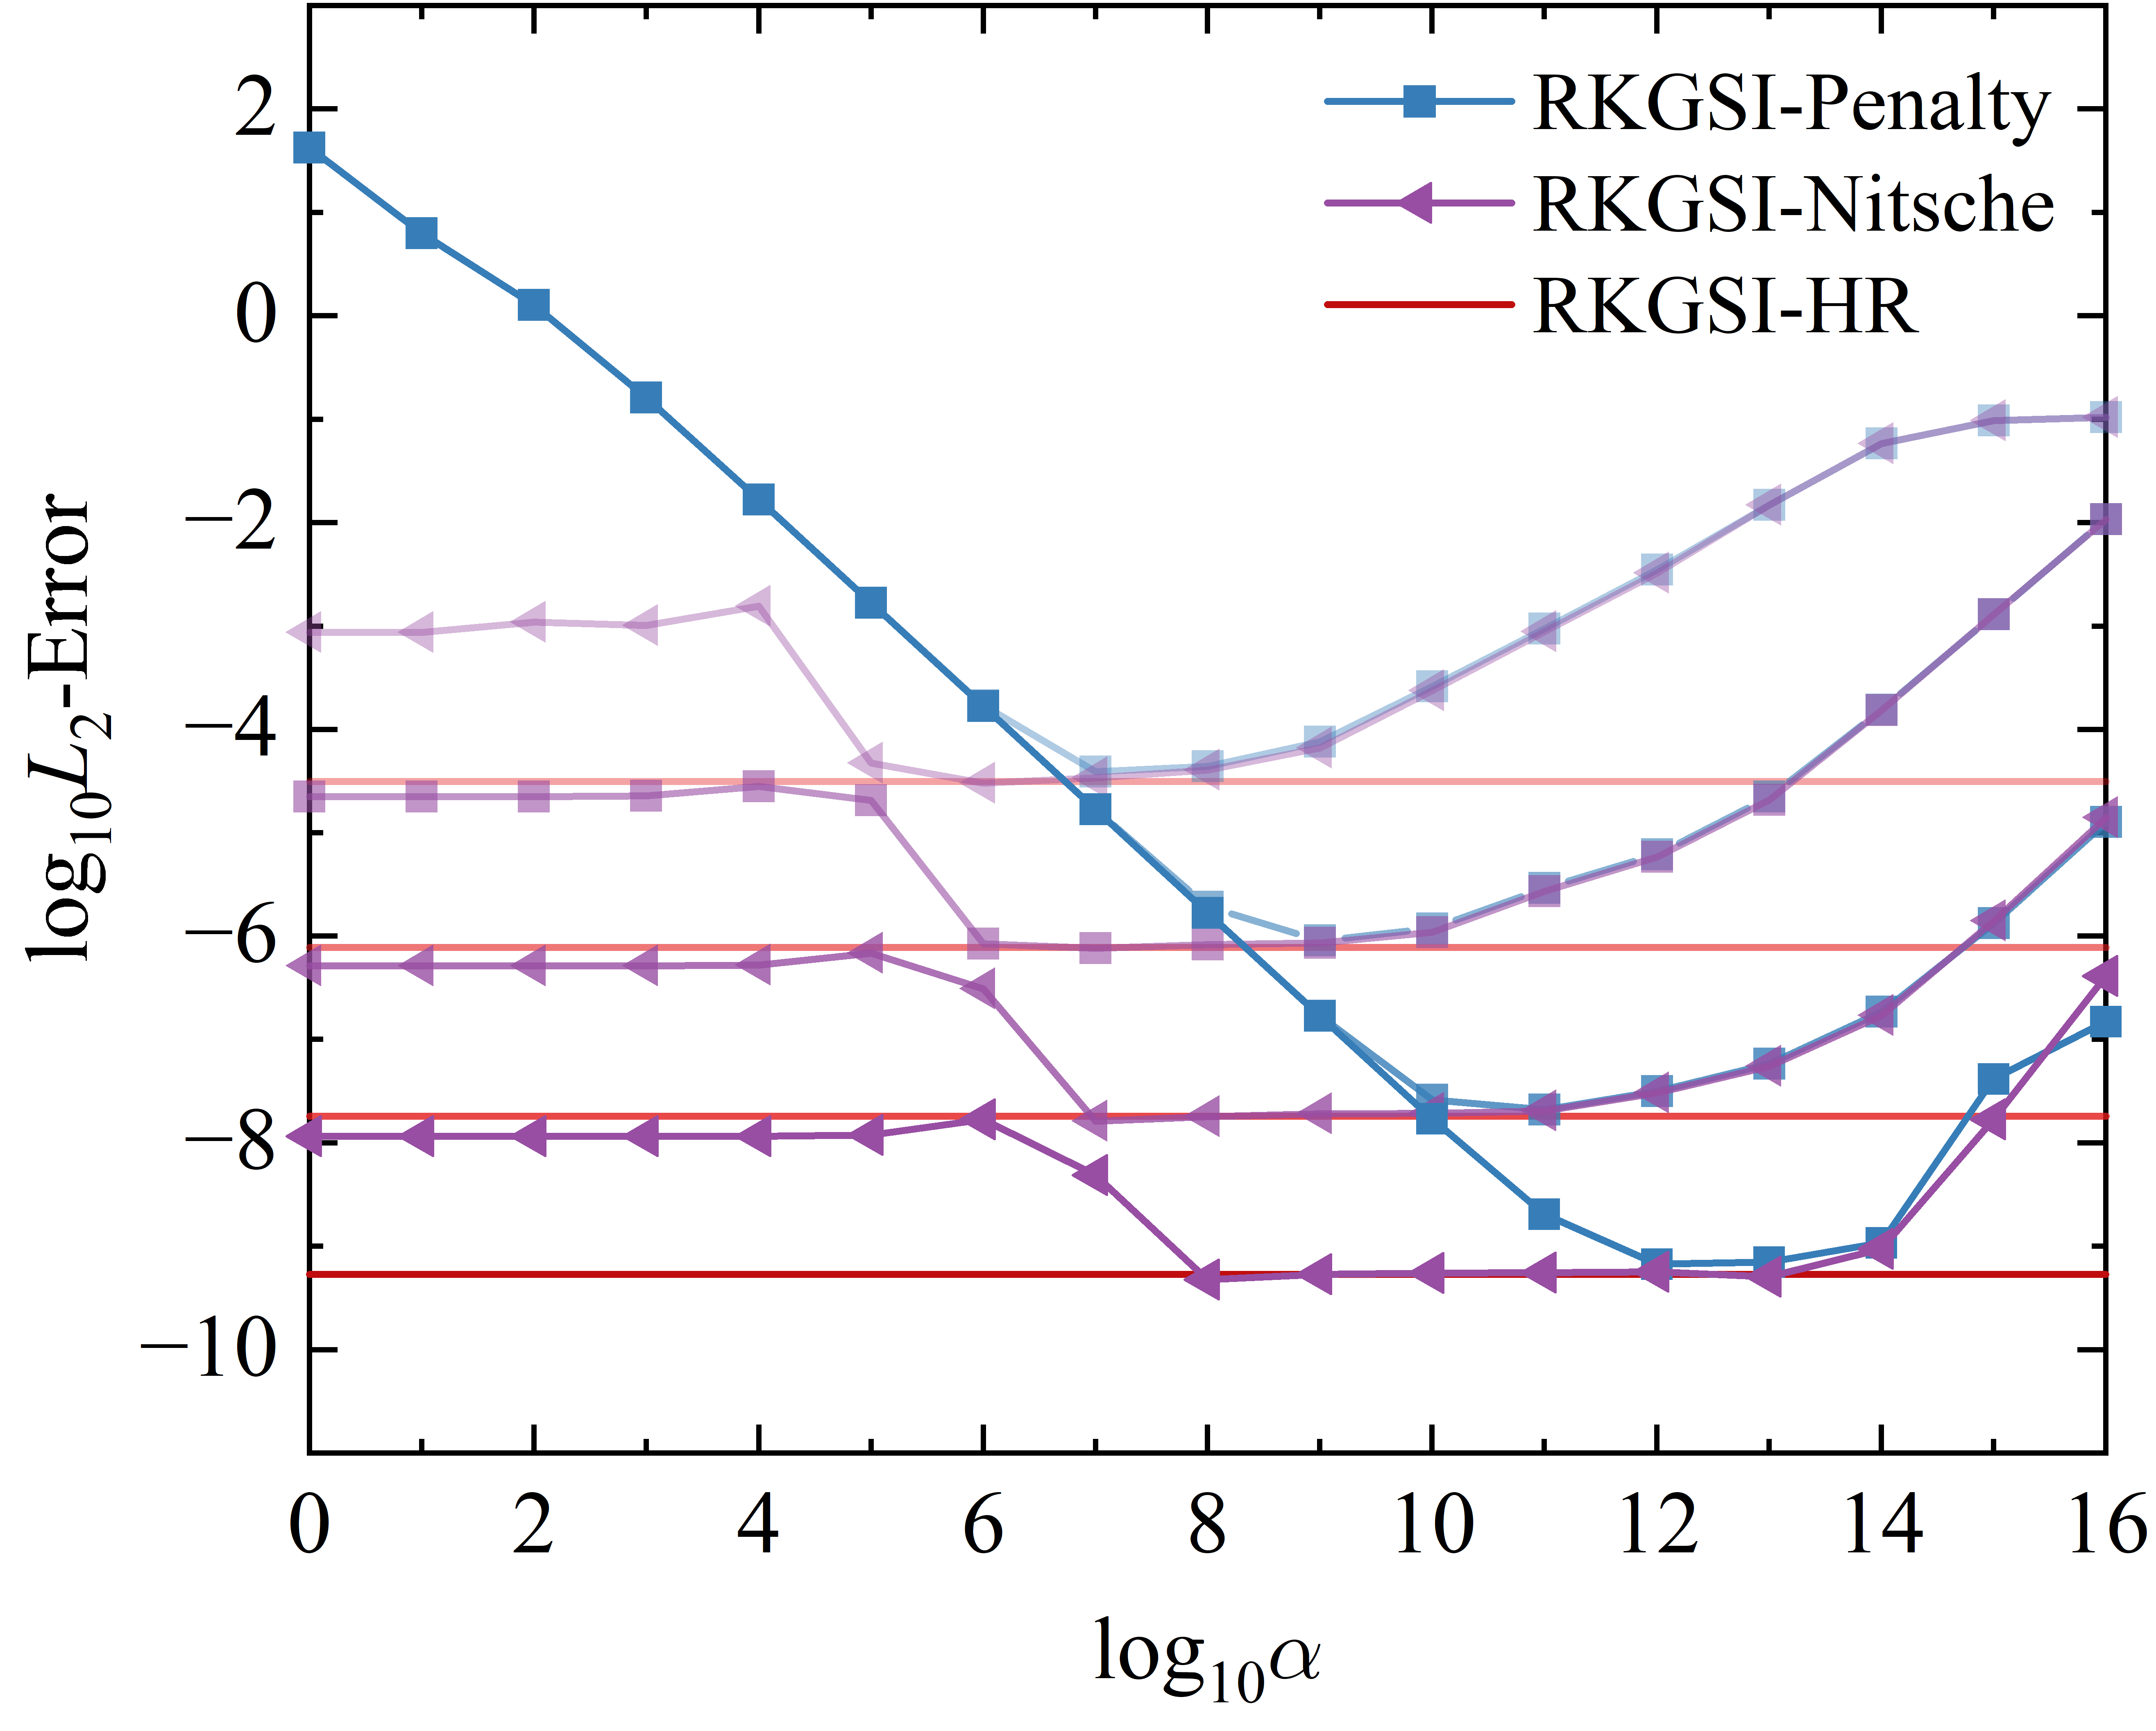
\includegraphics[width=0.49\textwidth]{figure/PHR/R/qalpha.png}
    \phantomcaption\label{qalpha}
    \end{subcaptiongroup}
\caption{人工参数$\alpha$敏感度分析:\subref{calpha}三次基函数;\subref{qalpha}四次基函数}
\label{Ralpha}
\end{figure}
\newpage
\subsection{简支等边三角形板问题}
一简支等边三角形板如图(\ref{triangular})所示,其中,三角形板的高为$a=10$,均布荷载作用在板面内为$\bar{q}=1$,材料系数分别为弯曲刚度$\bar{D}=1$、泊松比$\nu=0.3$。该简支三角形板的精确解为:
\begin{equation}
\begin{split}
    w=\frac{\bar q}{64a\bar D}[x^3-3y^3x-a(x^2+y^2)+\frac{4}{27}a^3](\frac{4}{9}a^2-x^2-y^2)
\end{split}
\end{equation}\par
如图(\ref{triangularmsh})所示,简支等边三角形板求解域分布采用均布离散的66、231、861和3321的四个疏密不同的节点进行离散。同样采用三次基函数时,简支等边三角形板问题的相对影响域取为3.5,四次基函数时其相对应影响域取为4.5进行数值分析。\par
\begin{figure}[H]
    \centering
    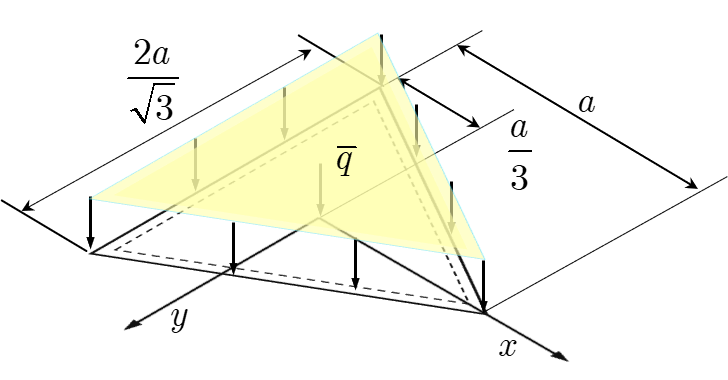
\includegraphics[scale=0.7]{figure/PHR/T/triangular.png}
    \caption{简支等边三角形板问题模型}\label{triangular}
\end{figure}
\begin{figure}[H]
    \centering
    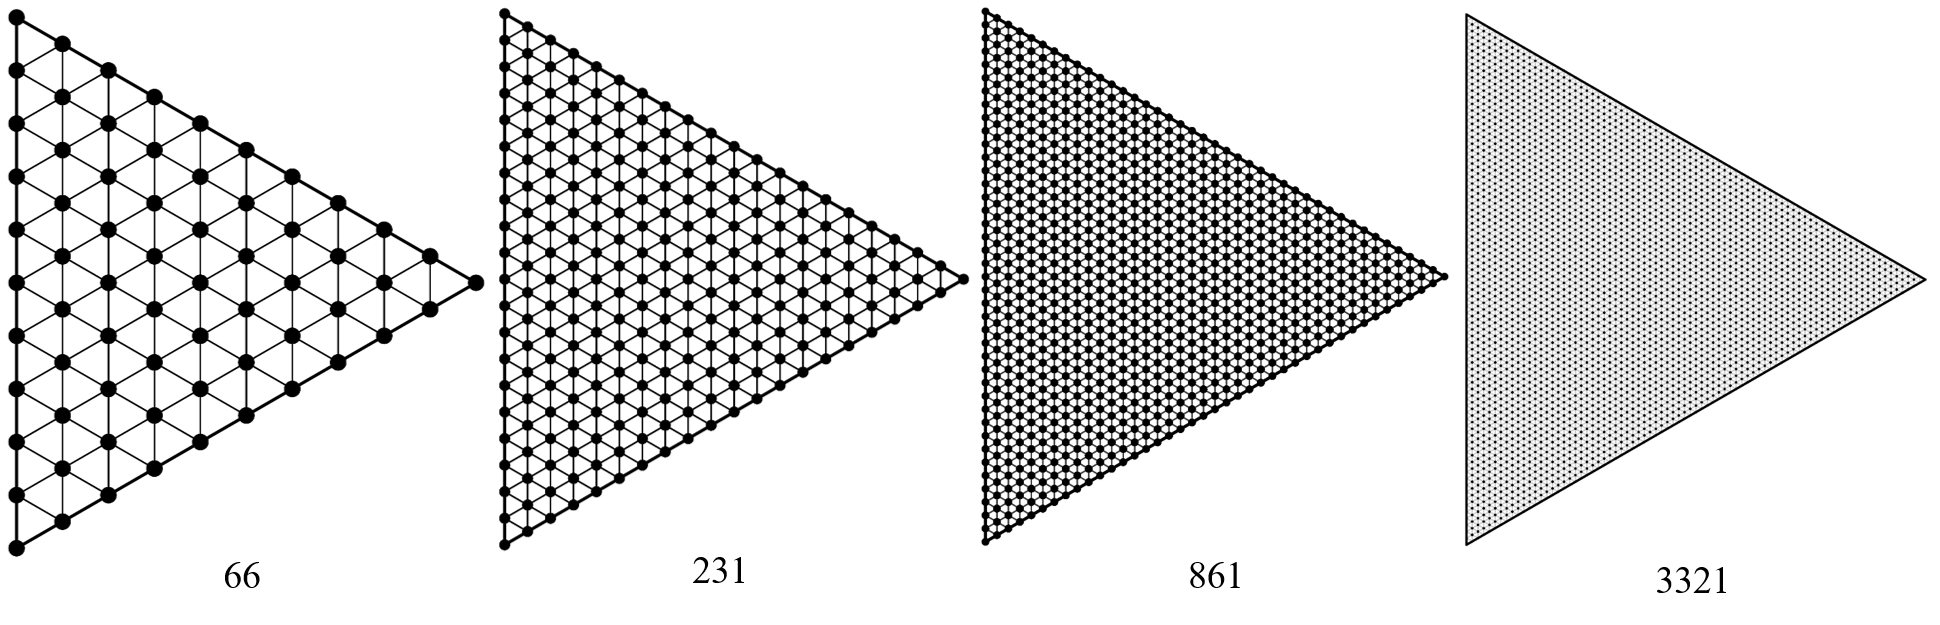
\includegraphics[scale=0.4]{figure/PHR/T/triangularmsh.png}
    \caption{简支等边三角形问题节点离散}\label{triangularmsh}
\end{figure}
图(\ref{TCLH})和图(\ref{TQLH})为简支等边三角形板问题分别在三次基函数和四次基函数的位移误差和能量误差对比图。从图中可以明显看出采用“RKGSI”得出的计算精度优于“GI”法。
并且不管是三次基函数还是四次基函数“RKGSI-Nitsche”、“RKGSI-HR”都能够达到理论误差收敛率,满足积分约束条件。
图(\ref{Tefficiency})是简支等边三角形板的薄板中面和本质边界条件施加效率分析图,从图中可以看出在薄板中面施加过程中,“RKGSI”所用的时间都明显少于“GI”;
而针对“RKGSI”在施加本质边界过程中计算形函数及梯度和组装相对应的刚度矩阵和力向量中可以明显看出“RKGSI-Nistche”法所用的时间明显多于“RKGSI-HR”和“RKGSI-Penalty”,
虽然“RKGSI-HR”和“RKGSI-Penalty”的计算效率相差不大,但“RKGSI-Penalty”由于不具有变分一致性无法达到理论误差收敛率。因此相较于传统的本质边界条件施加方法,
“RKGSI-HR”不仅满足积分约束条件能够达到理论误差收敛率,提高计算精度,在计算时间上也用时较短,有效提高计算效率。
图(\ref{TMxy})为简支等边三角形板问题的弯矩云图。从图中可以看出“RKGSI-HR”、“RKGSI-Nitsche”和“RKGSI-Penalty”和精确解之间非常一致,进一步验证了所提方法能够有效提高计算精度。
\begin{figure}[H]
    \centering
    \begin{subcaptiongroup}
    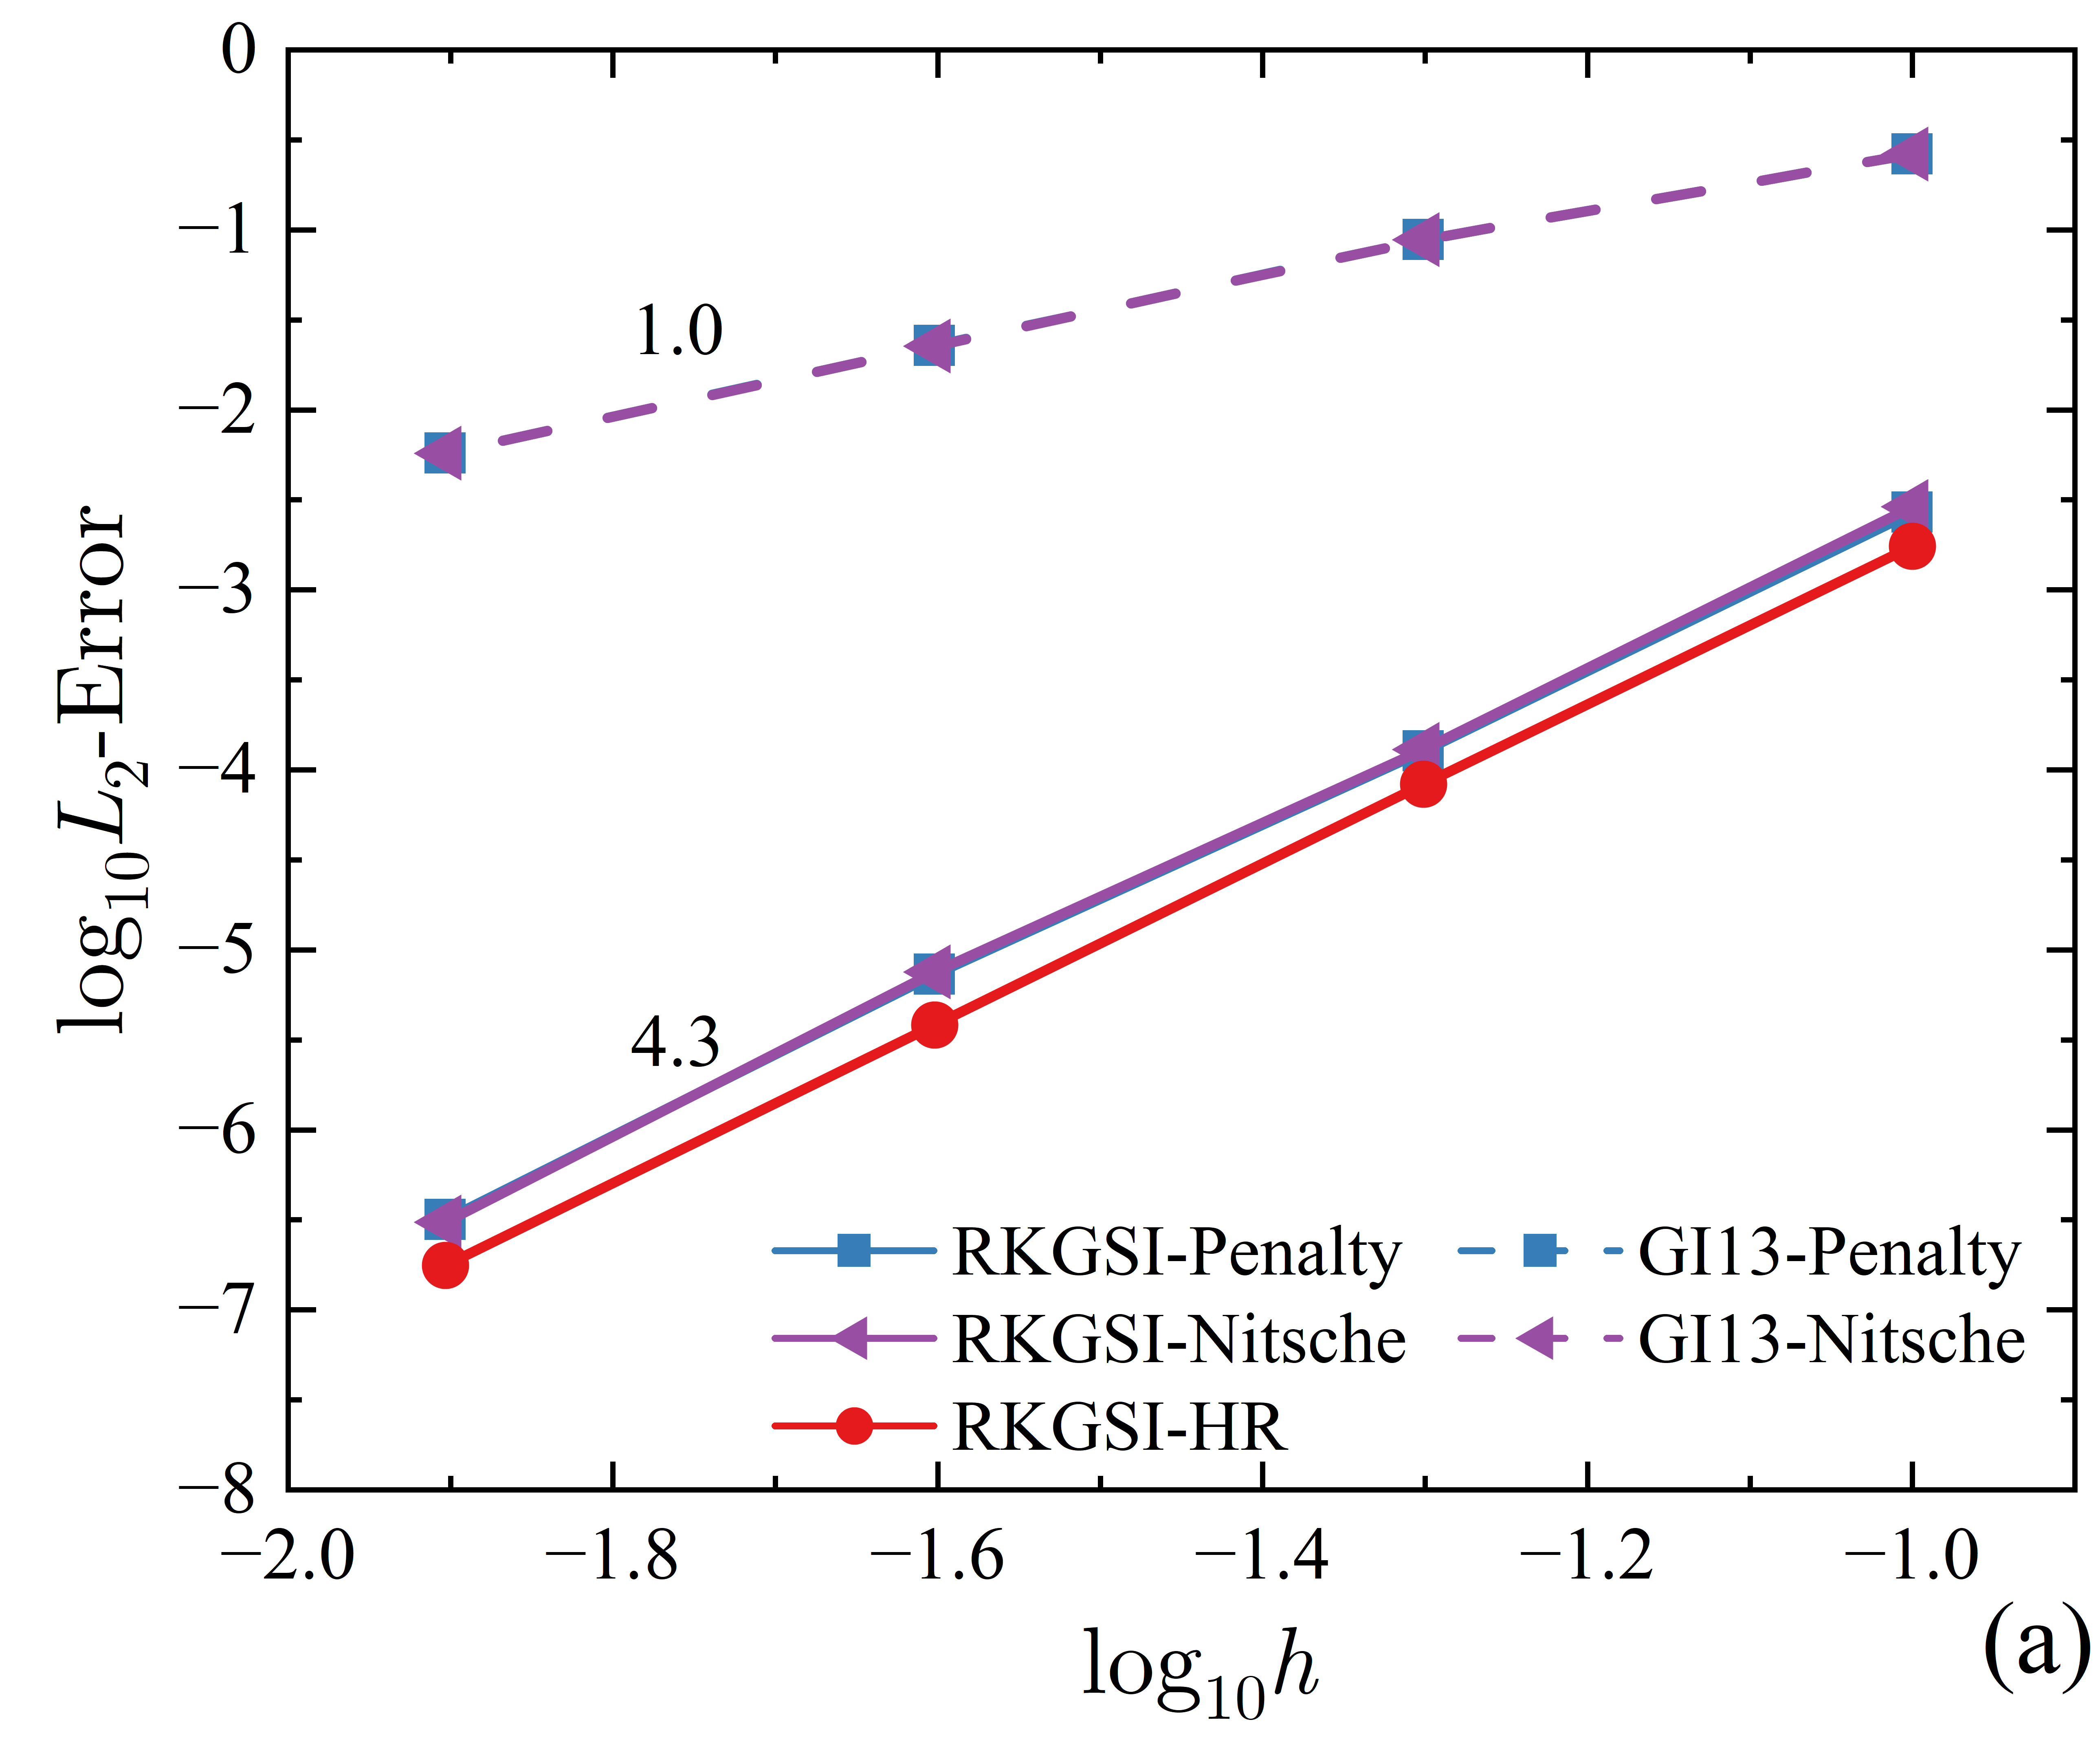
\includegraphics[width=0.49\textwidth]{figure/PHR/T/CL2.png}
    \phantomcaption\label{CL2}
    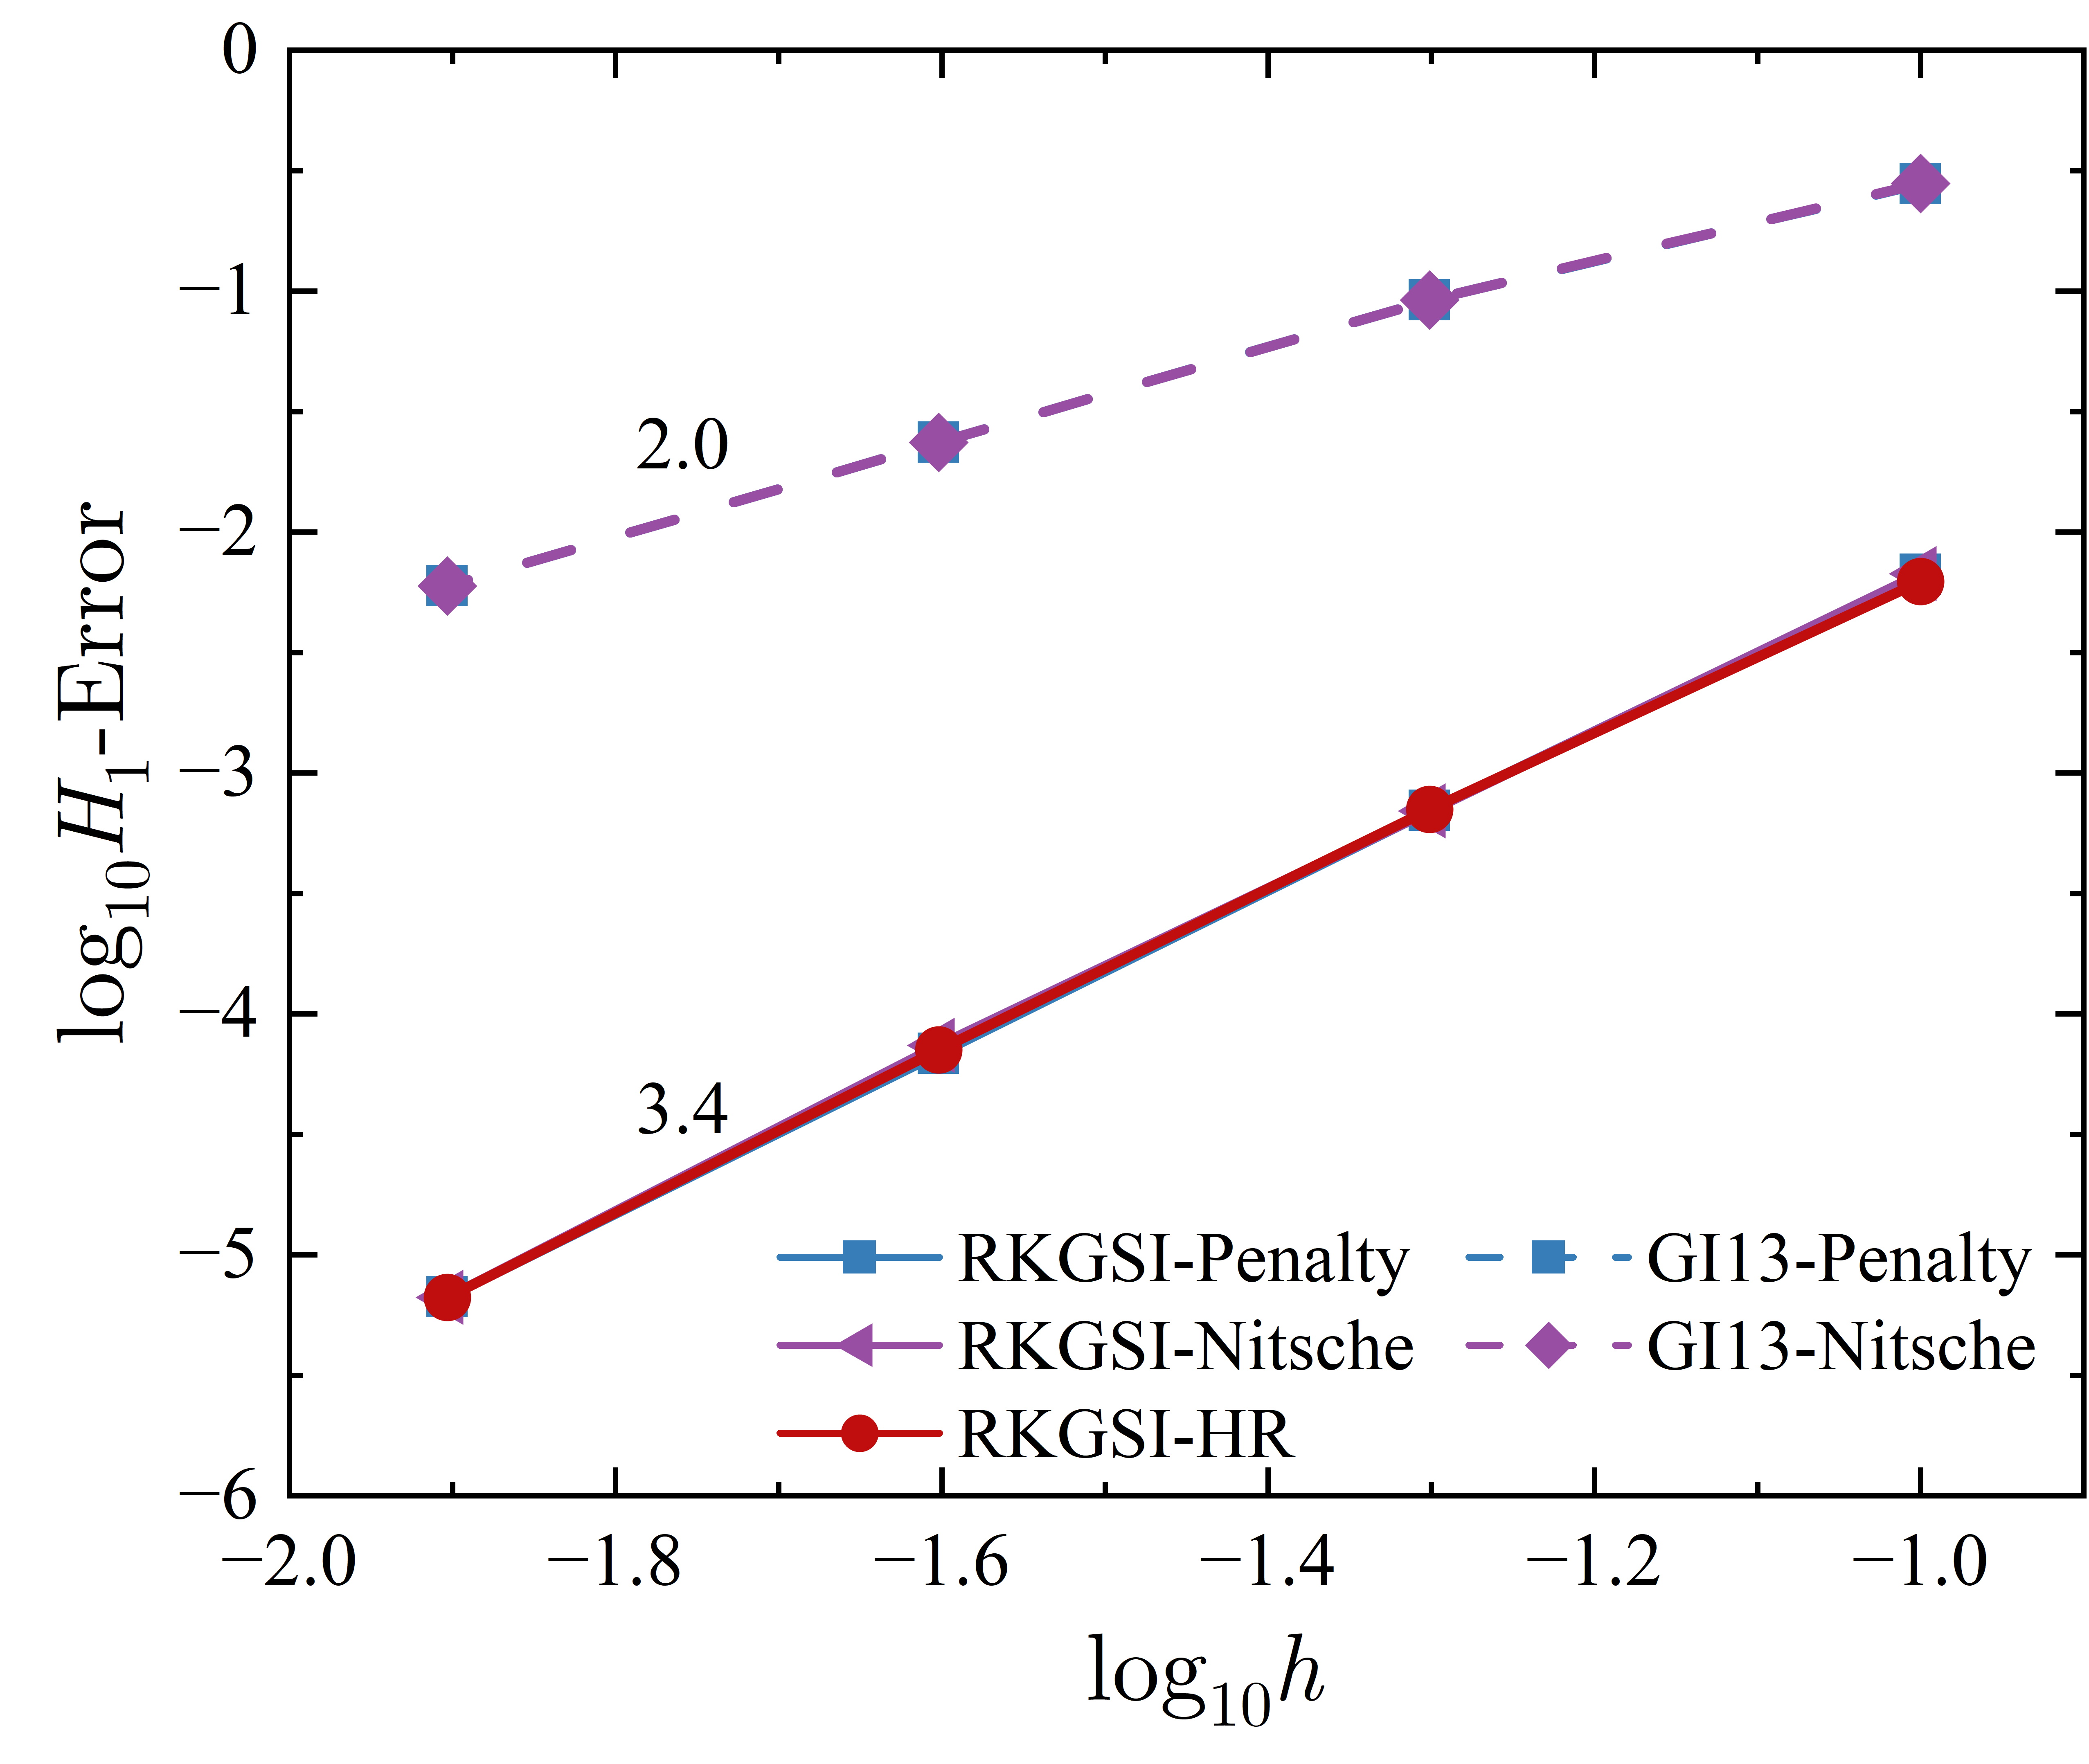
\includegraphics[width=0.49\textwidth]{figure/PHR/T/CH1.png}
    \phantomcaption\label{CH1}
    \end{subcaptiongroup}
    \begin{subcaptiongroup}
    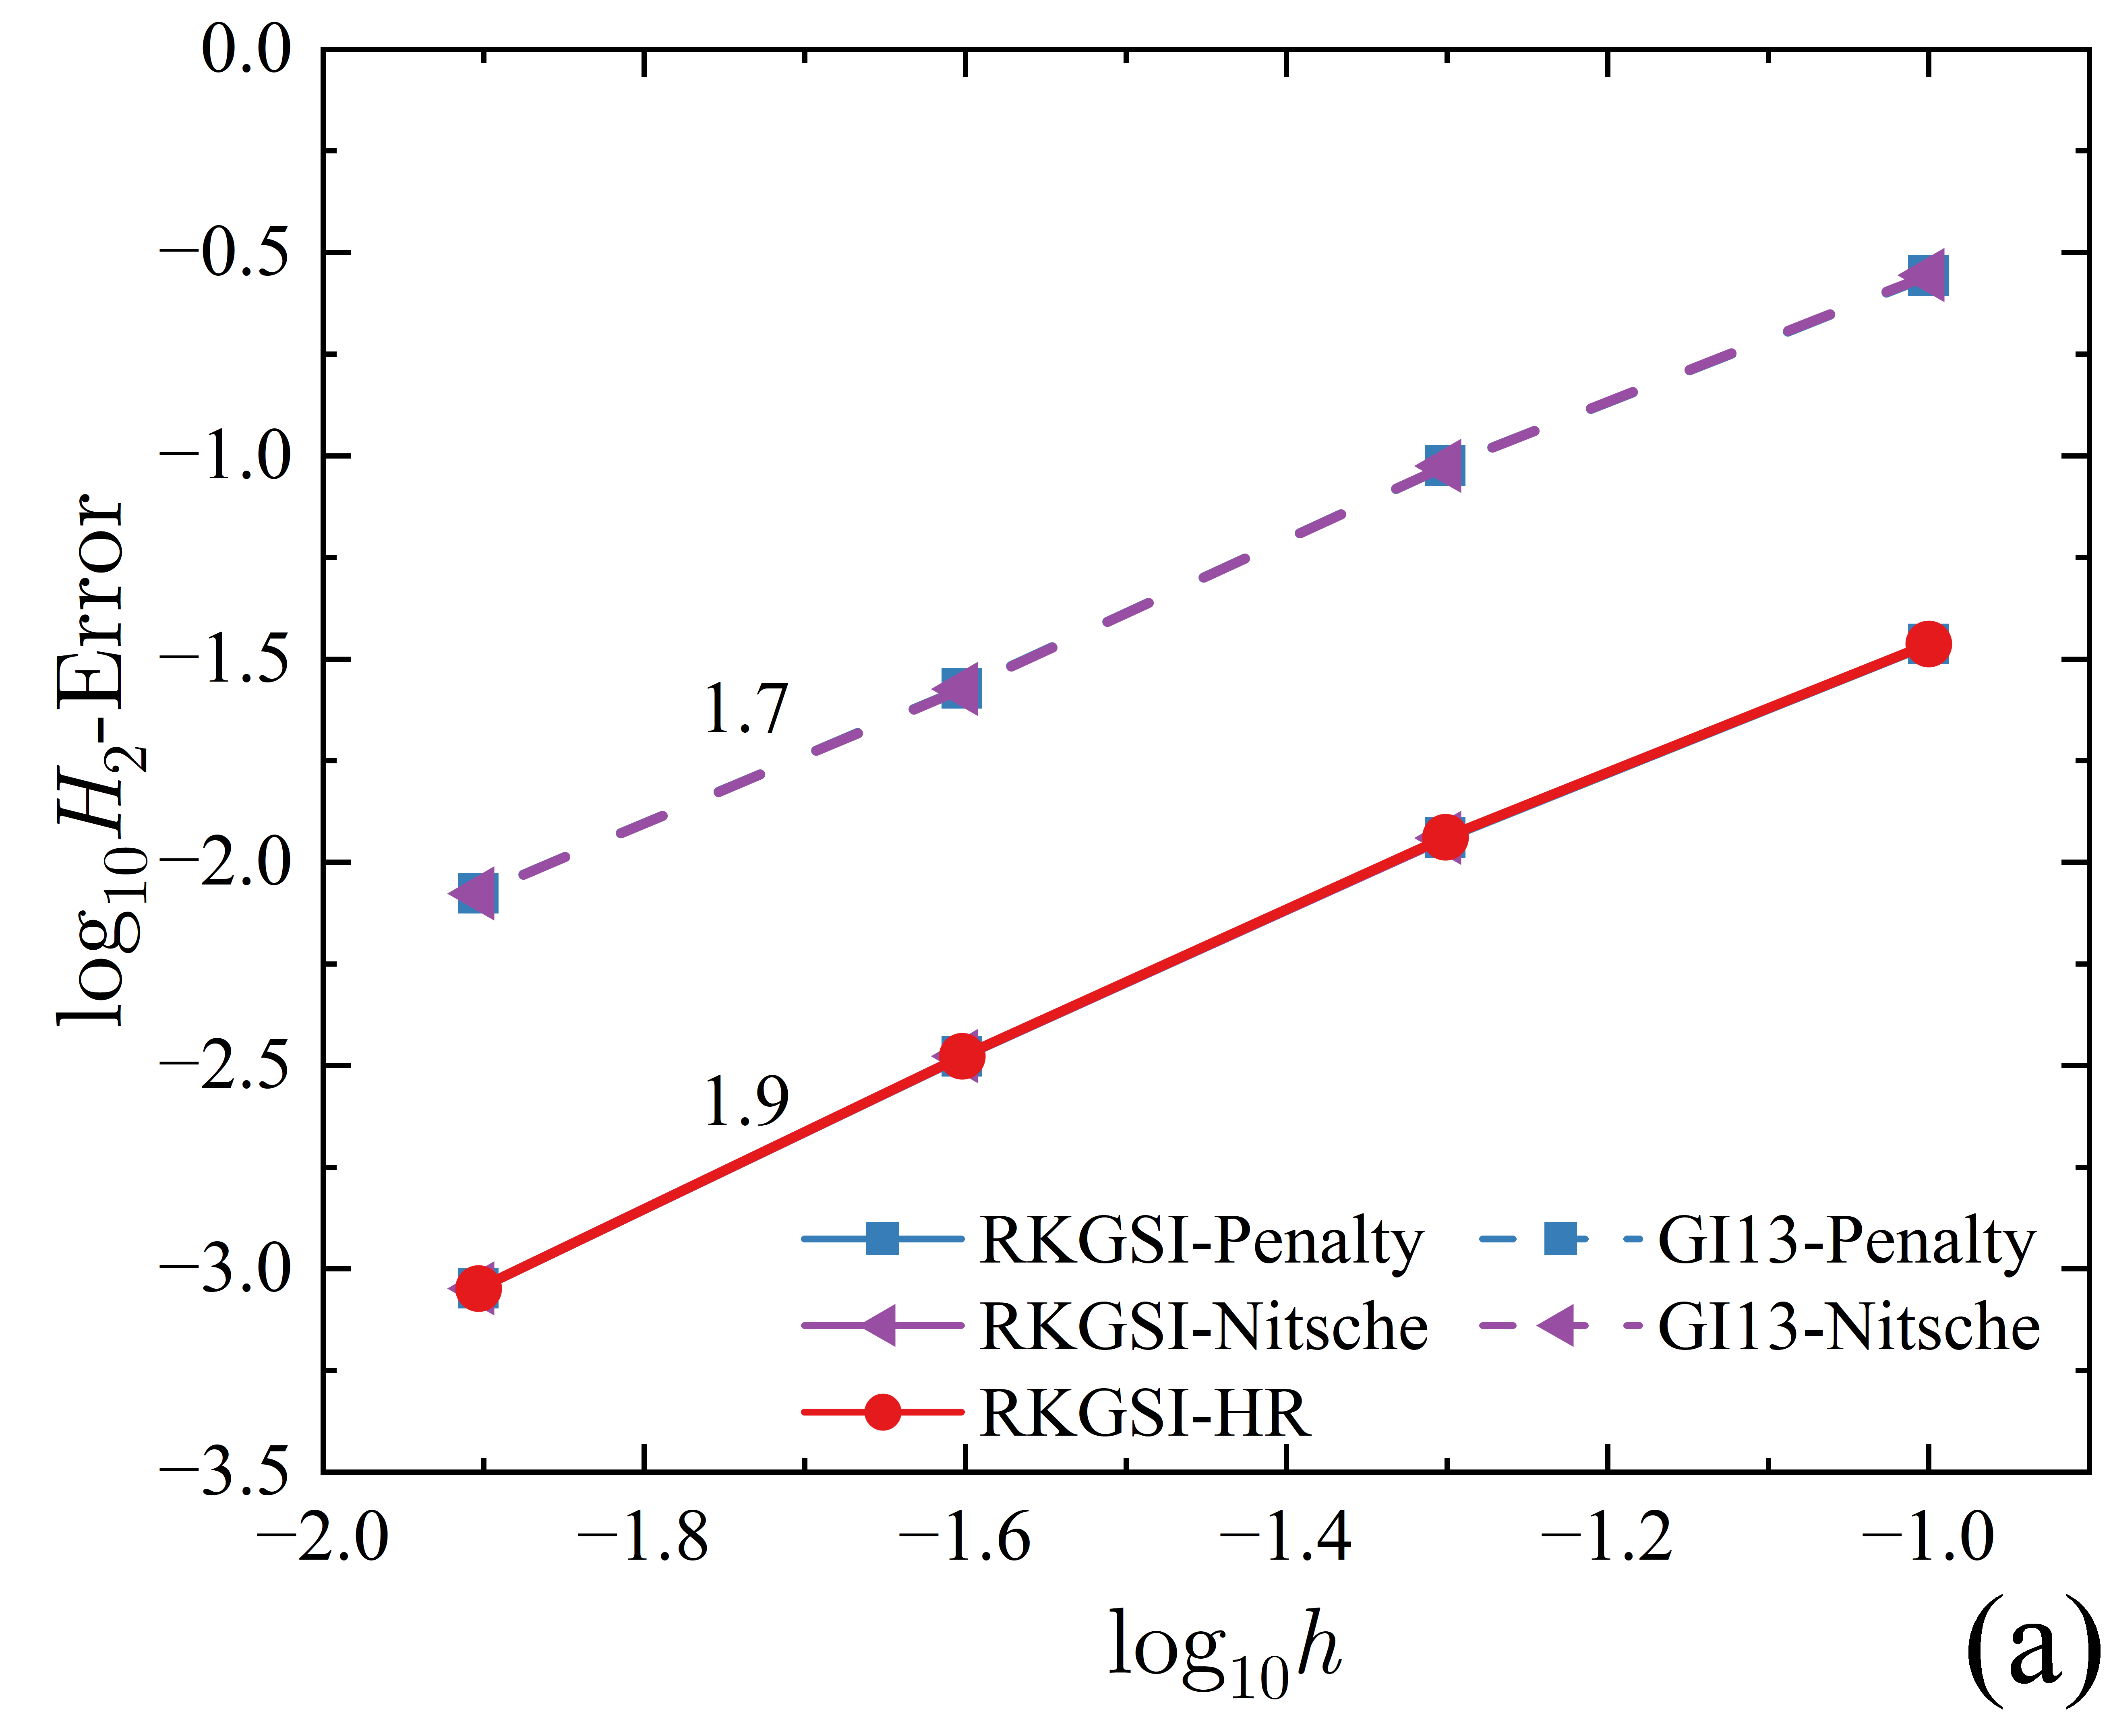
\includegraphics[width=0.49\textwidth]{figure/PHR/T/CH2.png}
    \phantomcaption\label{CH2}
    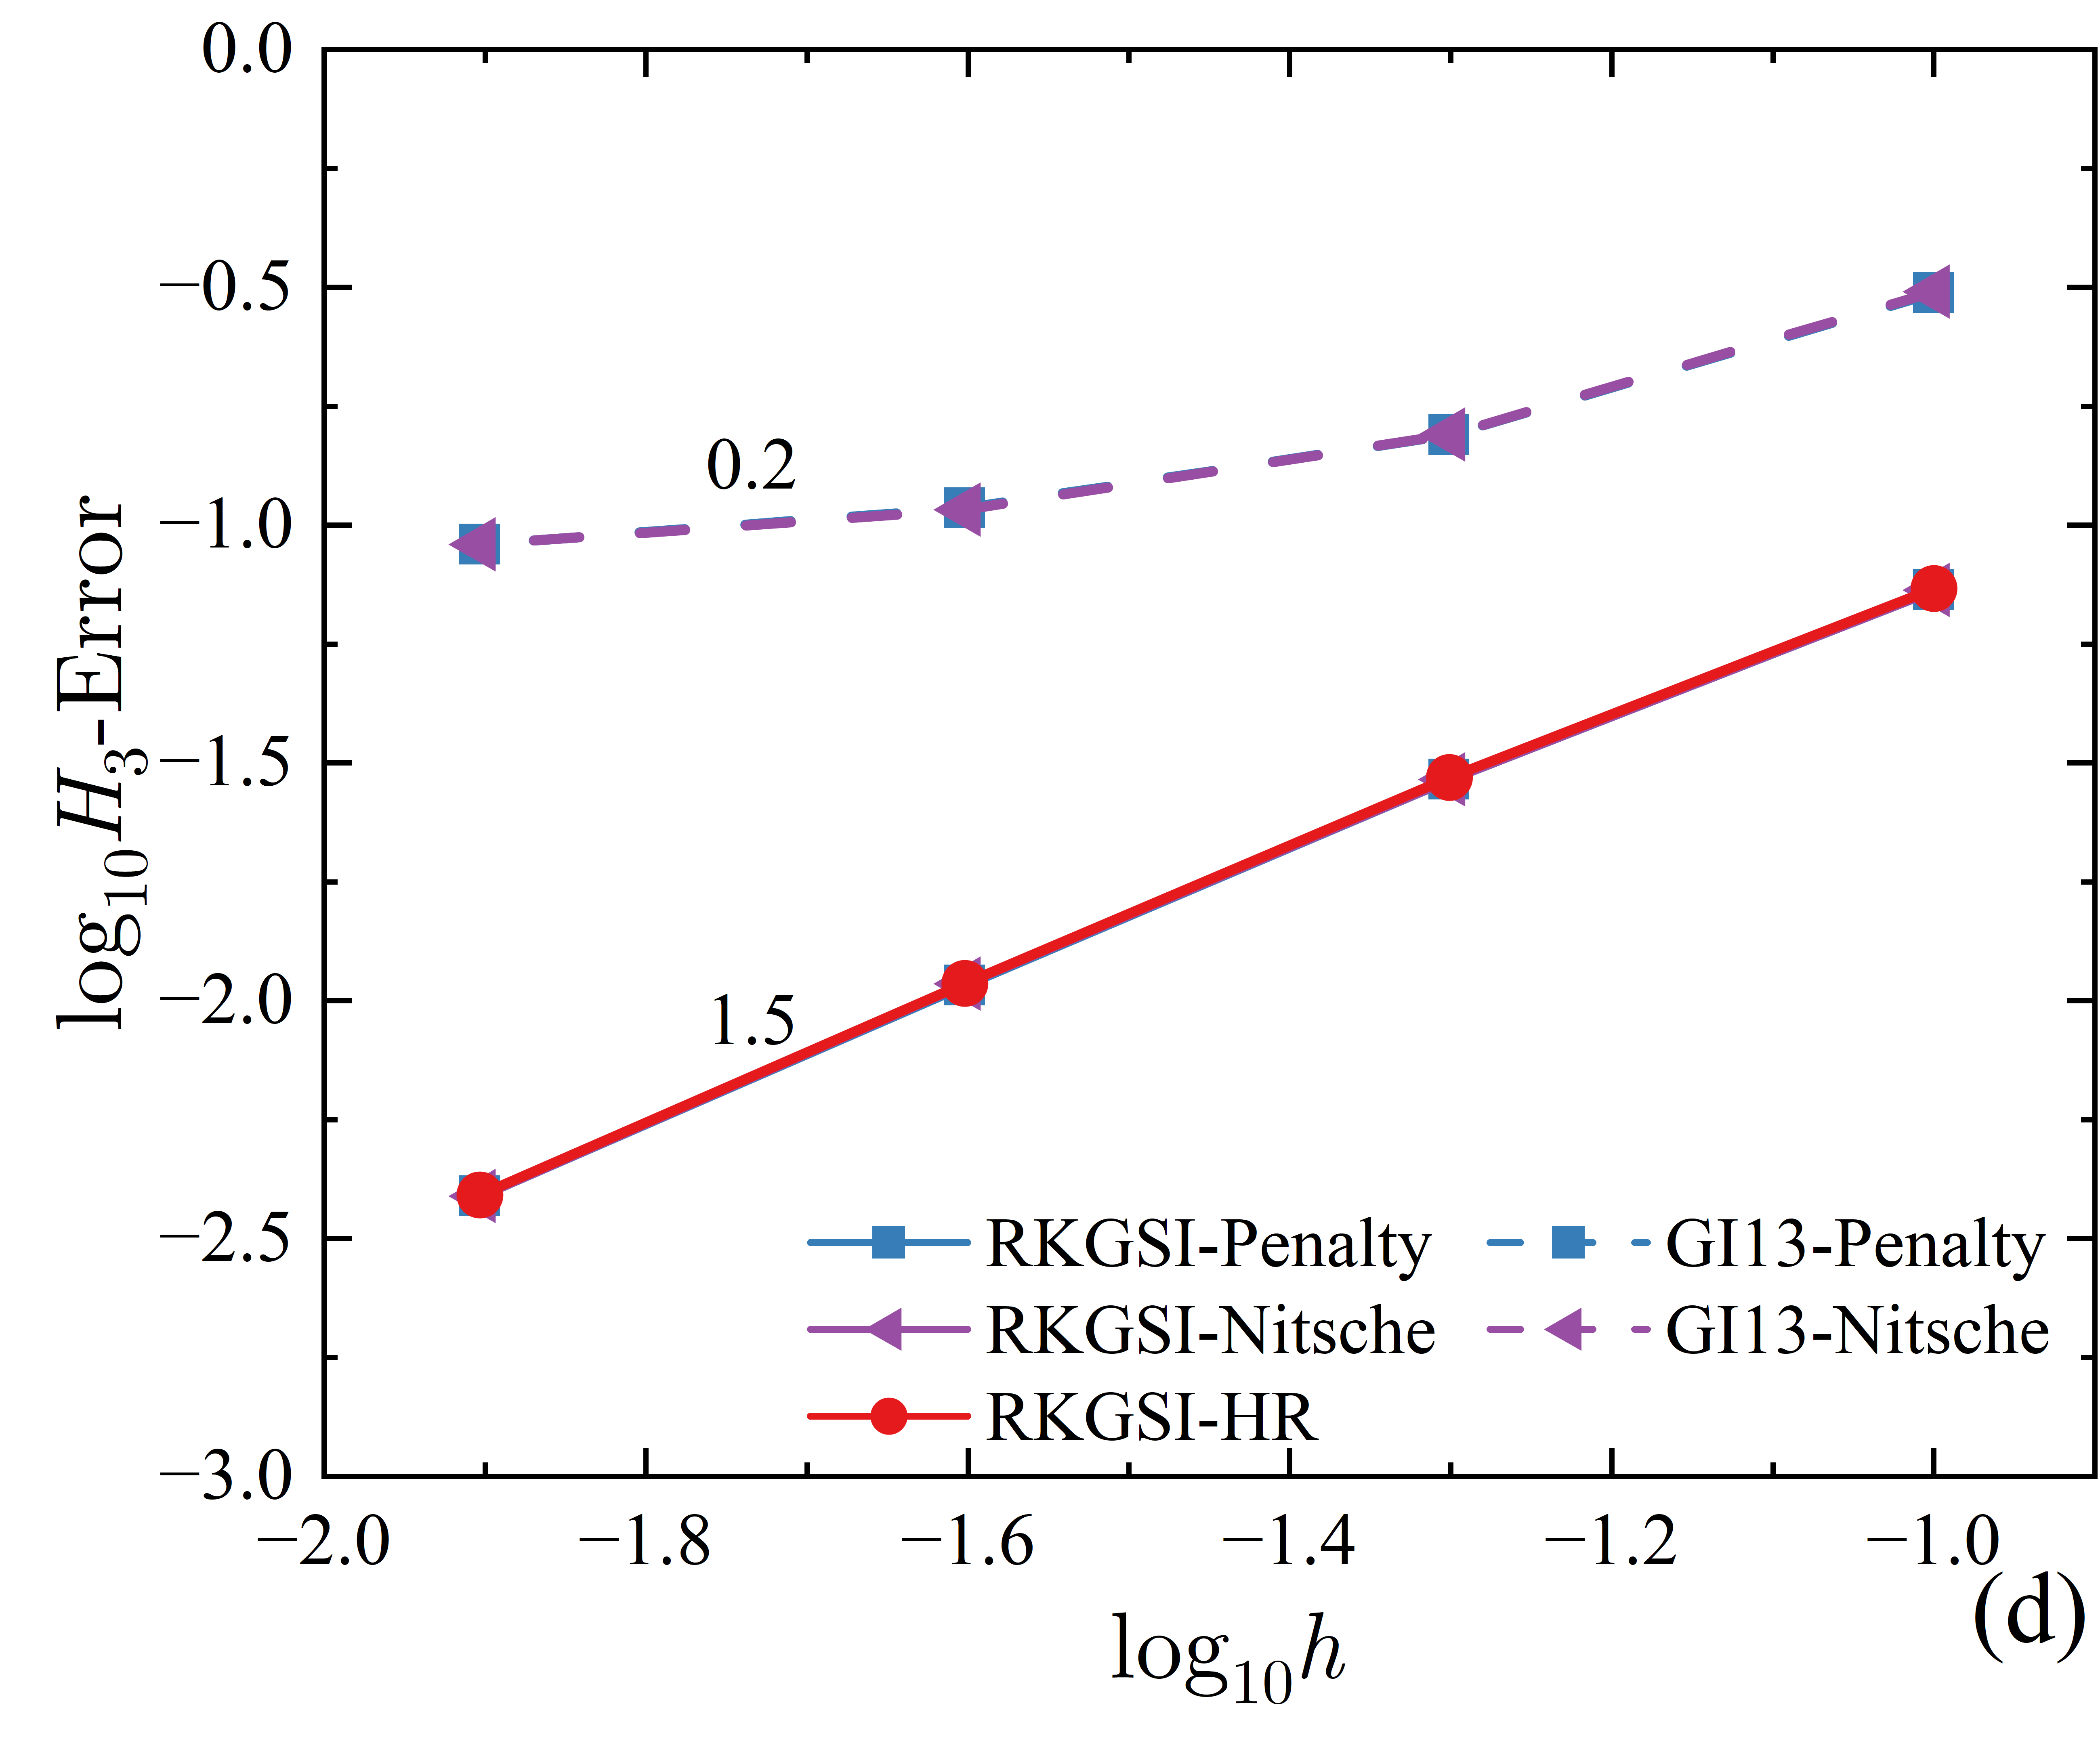
\includegraphics[width=0.49\textwidth]{figure/PHR/T/CH3.png}
    \phantomcaption\label{CH3}
    \end{subcaptiongroup}
\caption{简支等边三角形板问题三次基函数误差对比:\subref{CL2} $L_2$误差;\subref{CH1} $H_1$;误差\subref{CH2};$H_2$误差;\subref{CH3} $H_3$误差}
\label{TCLH}
\end{figure}
\newpage
\begin{figure}[H]
    \centering
    \begin{subcaptiongroup}
    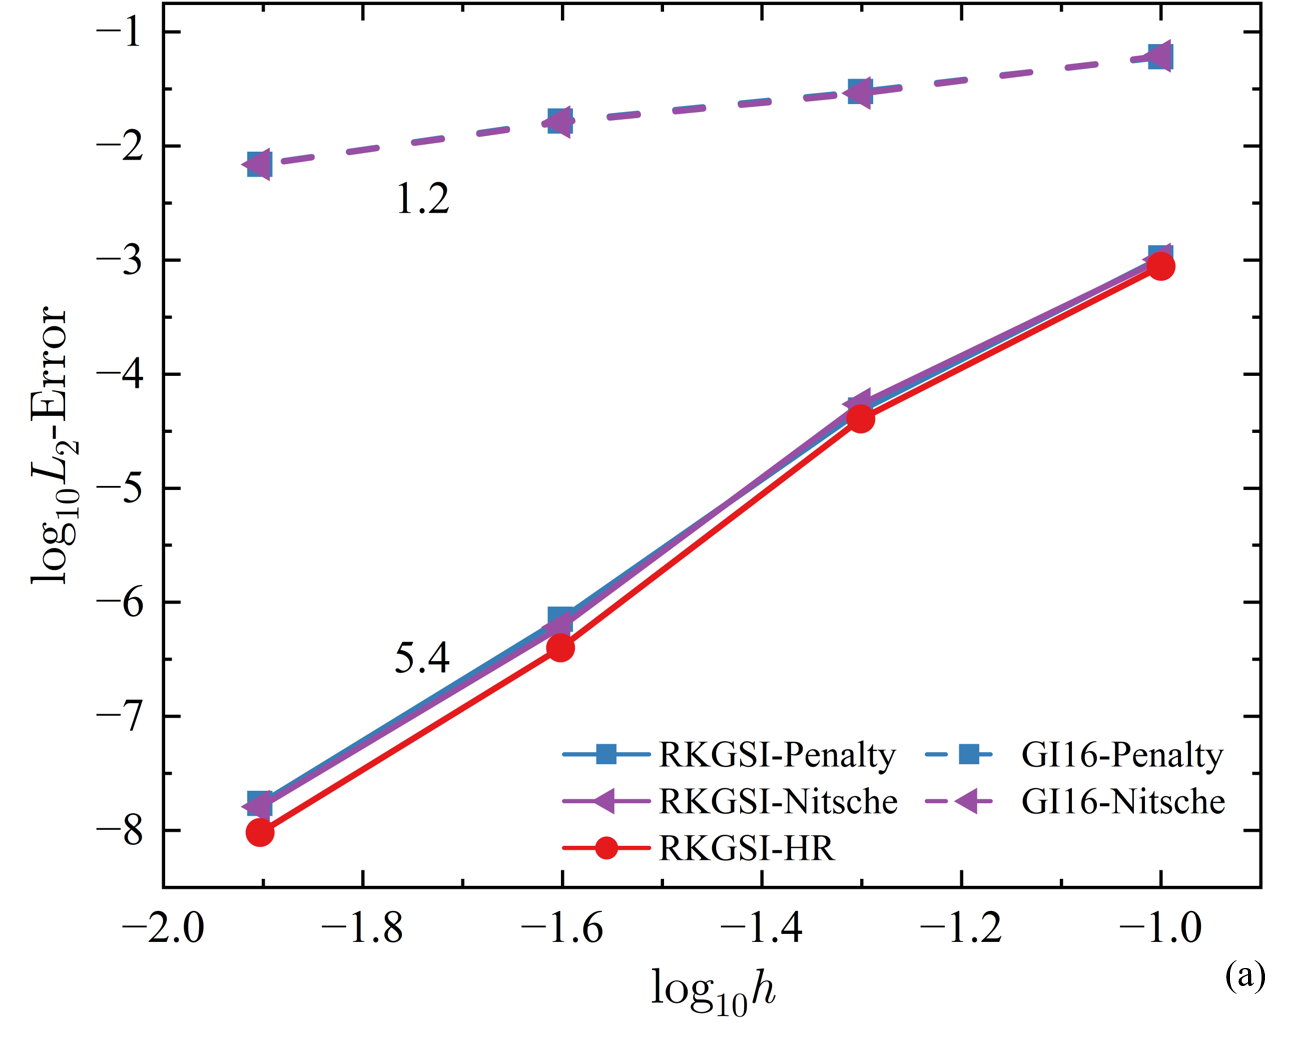
\includegraphics[width=0.49\textwidth]{figure/PHR/T/QL2.png}
    \phantomcaption\label{QL2}
    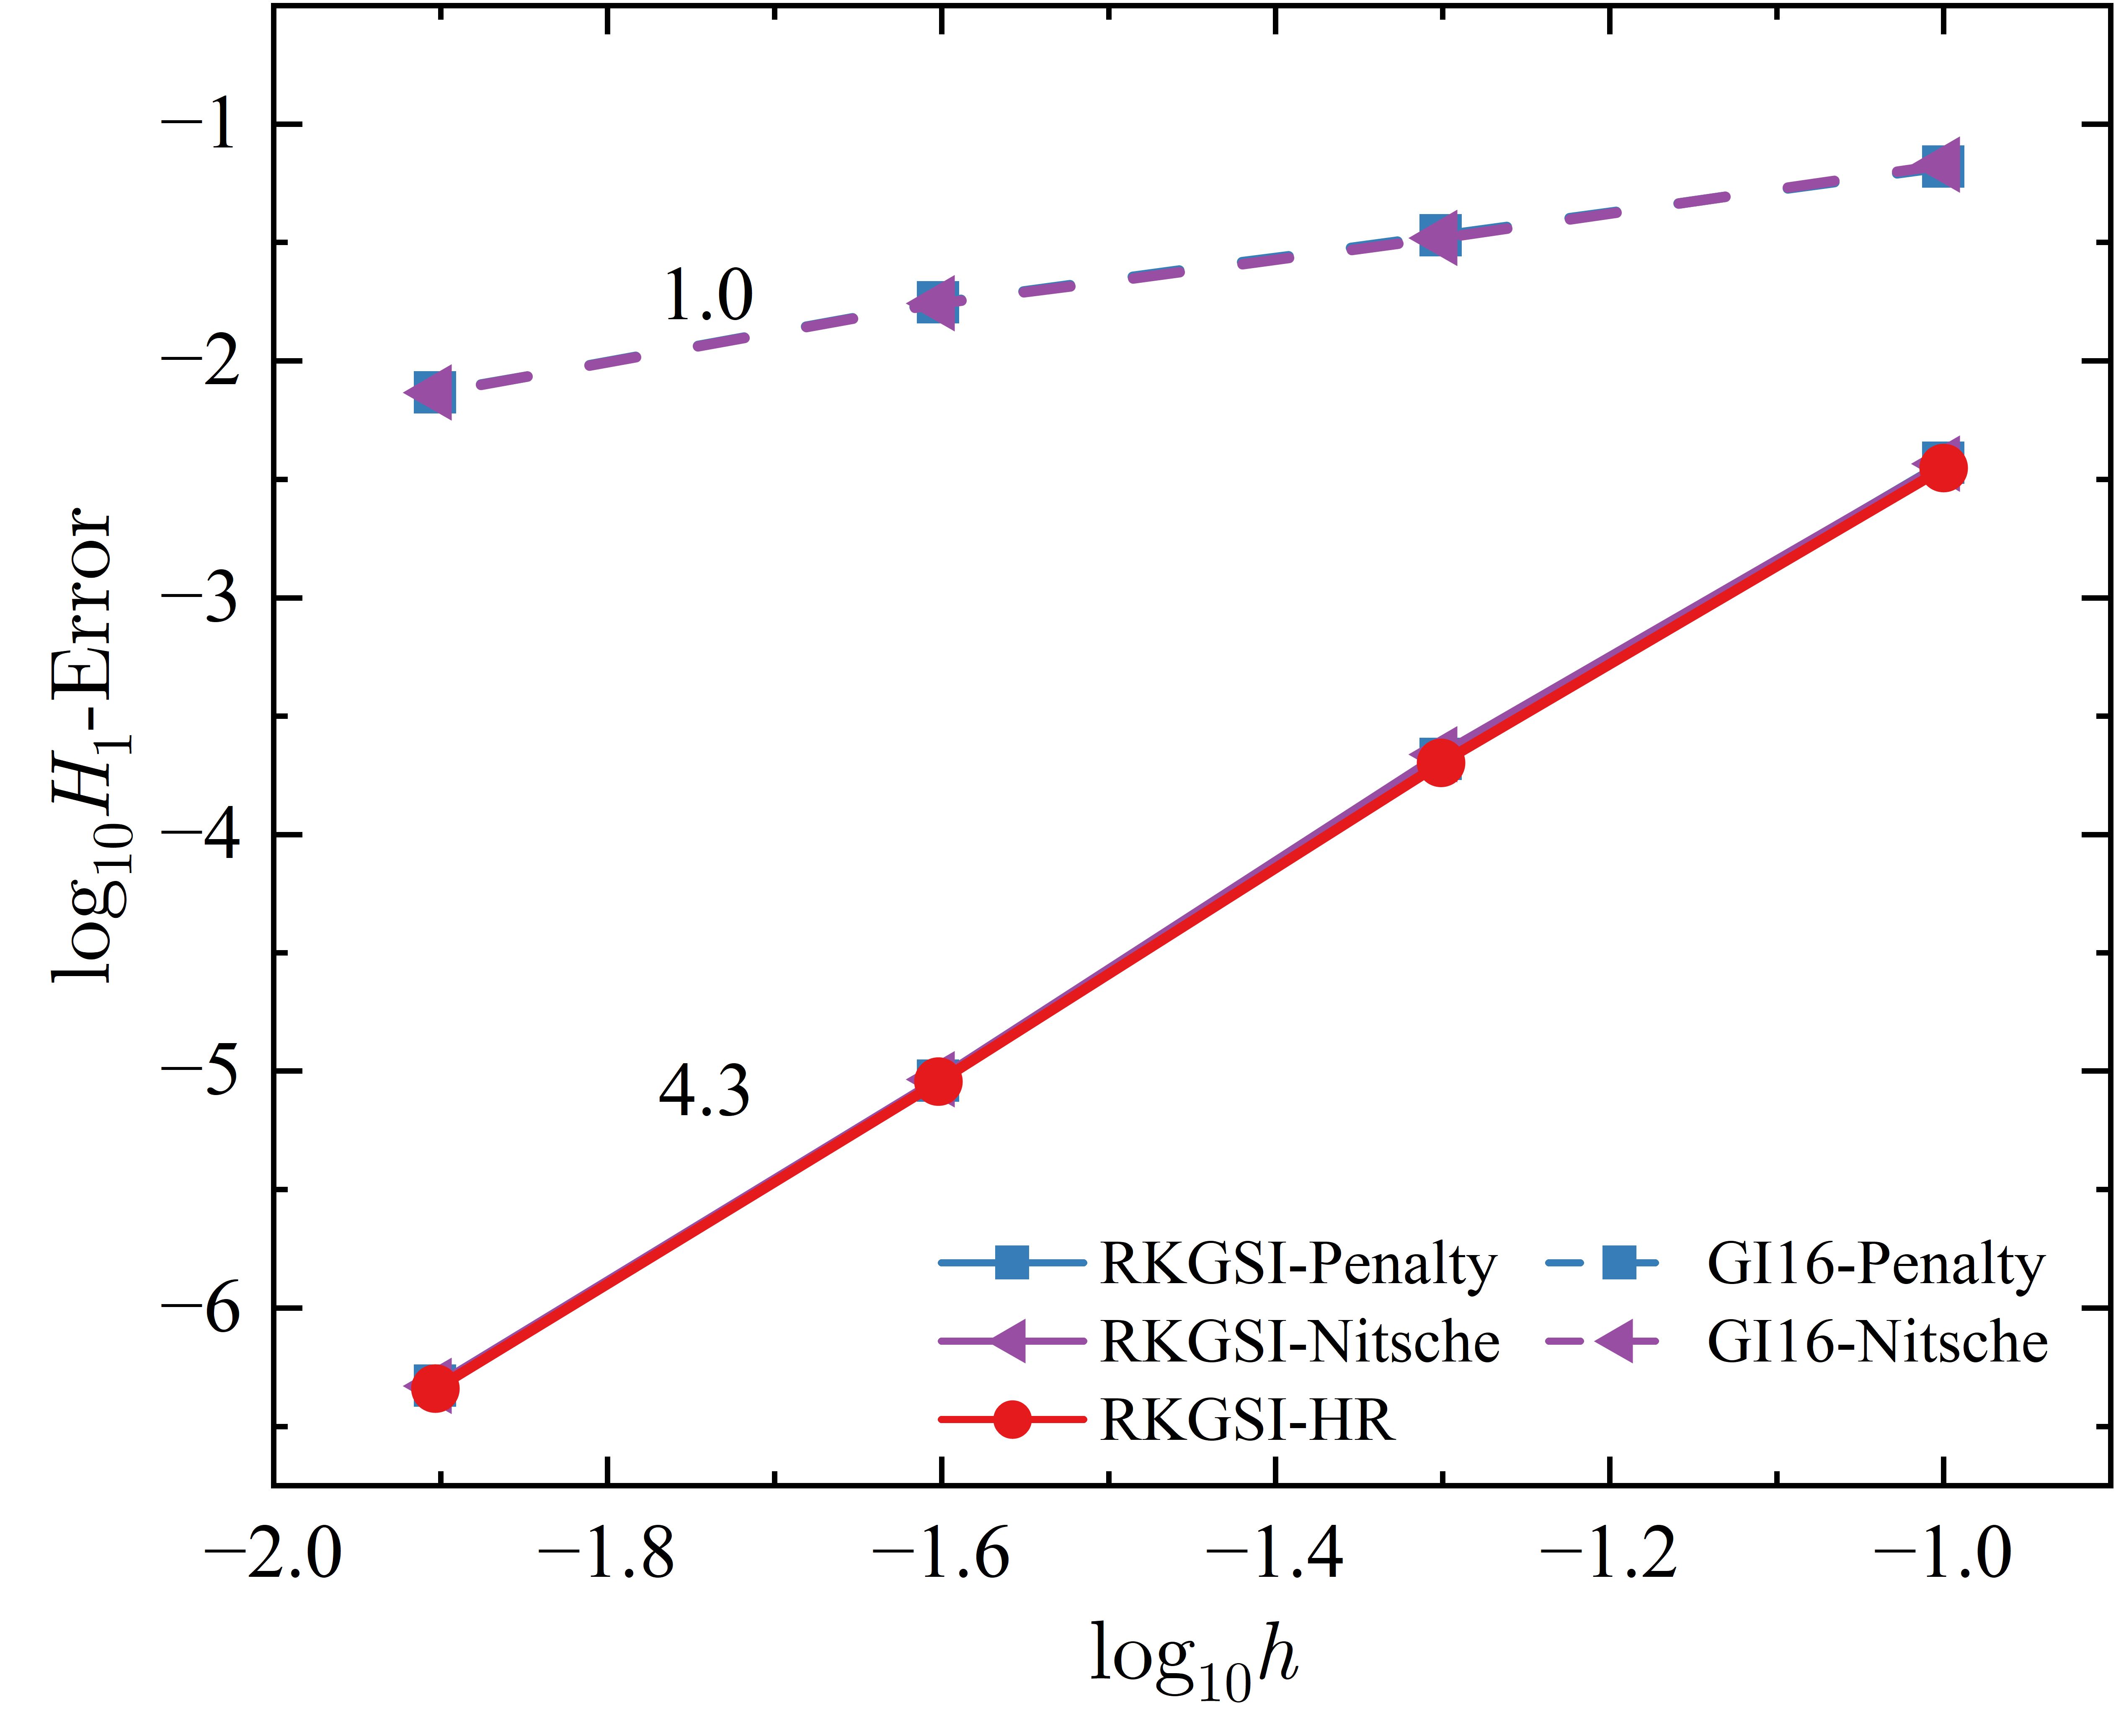
\includegraphics[width=0.49\textwidth]{figure/PHR/T/QH1.png}
    \phantomcaption\label{QH1}
    \end{subcaptiongroup}
    \begin{subcaptiongroup}
    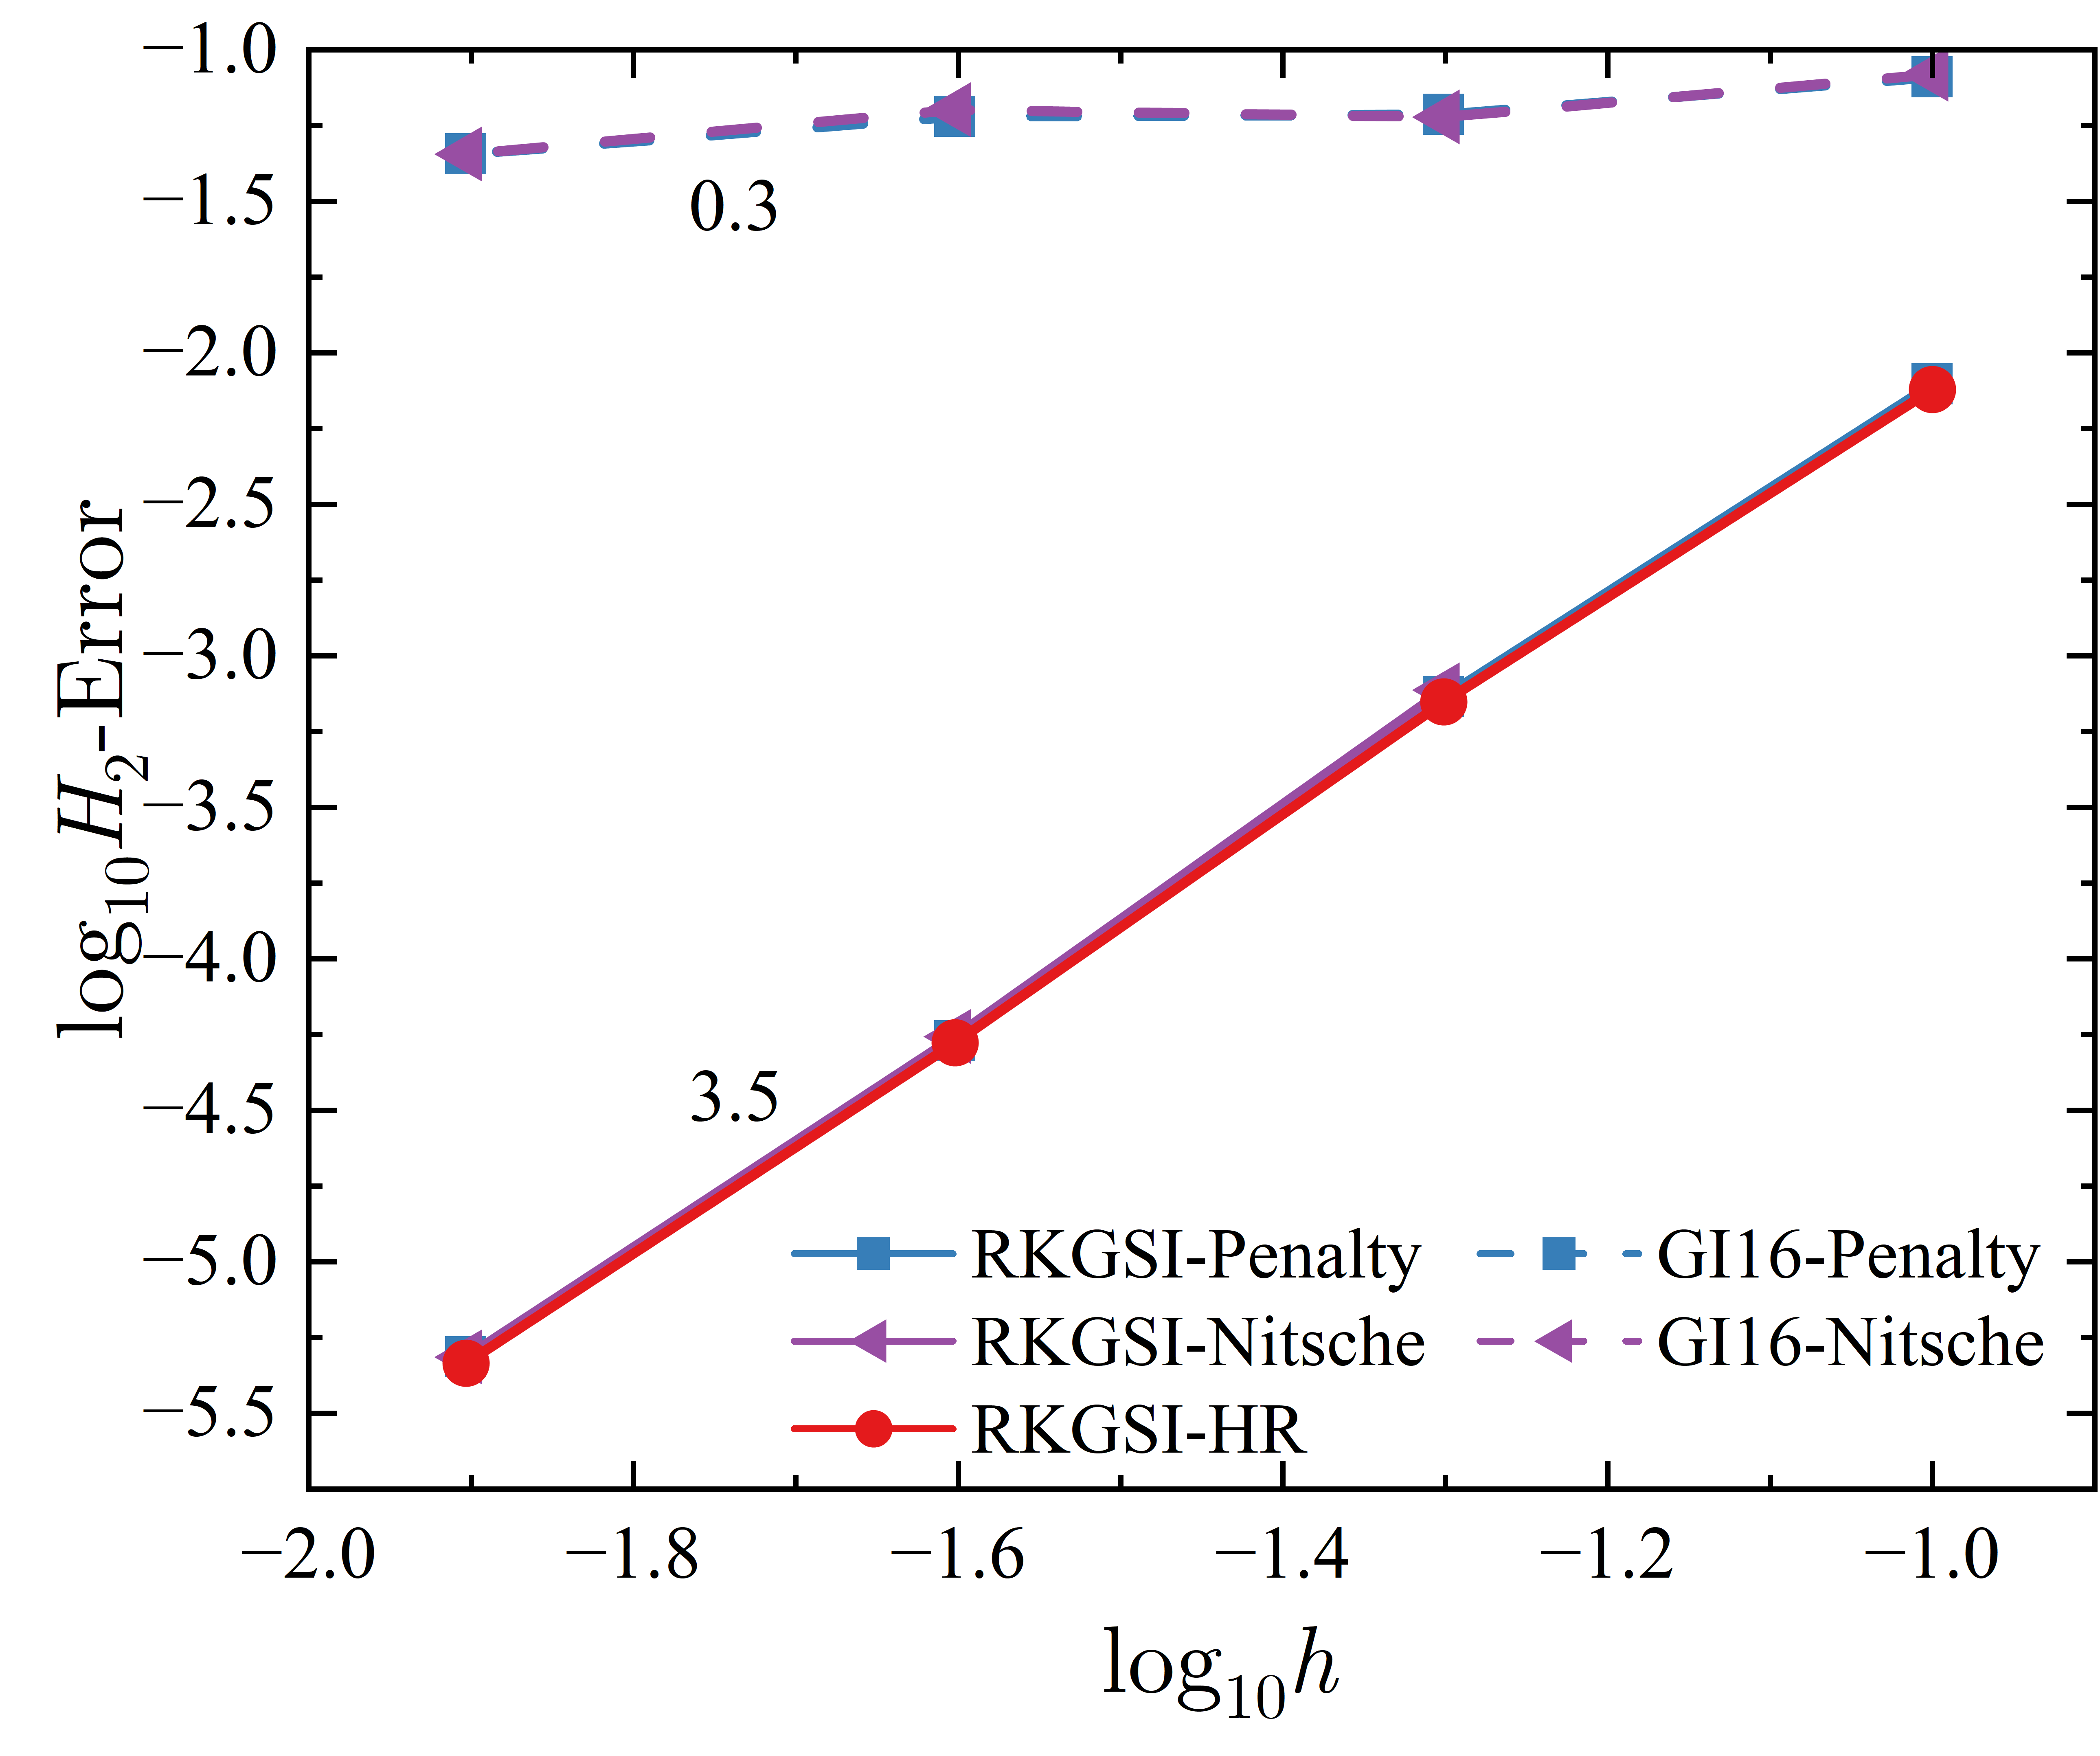
\includegraphics[width=0.49\textwidth]{figure/PHR/T/QH2.png}
    \phantomcaption\label{QH2}
    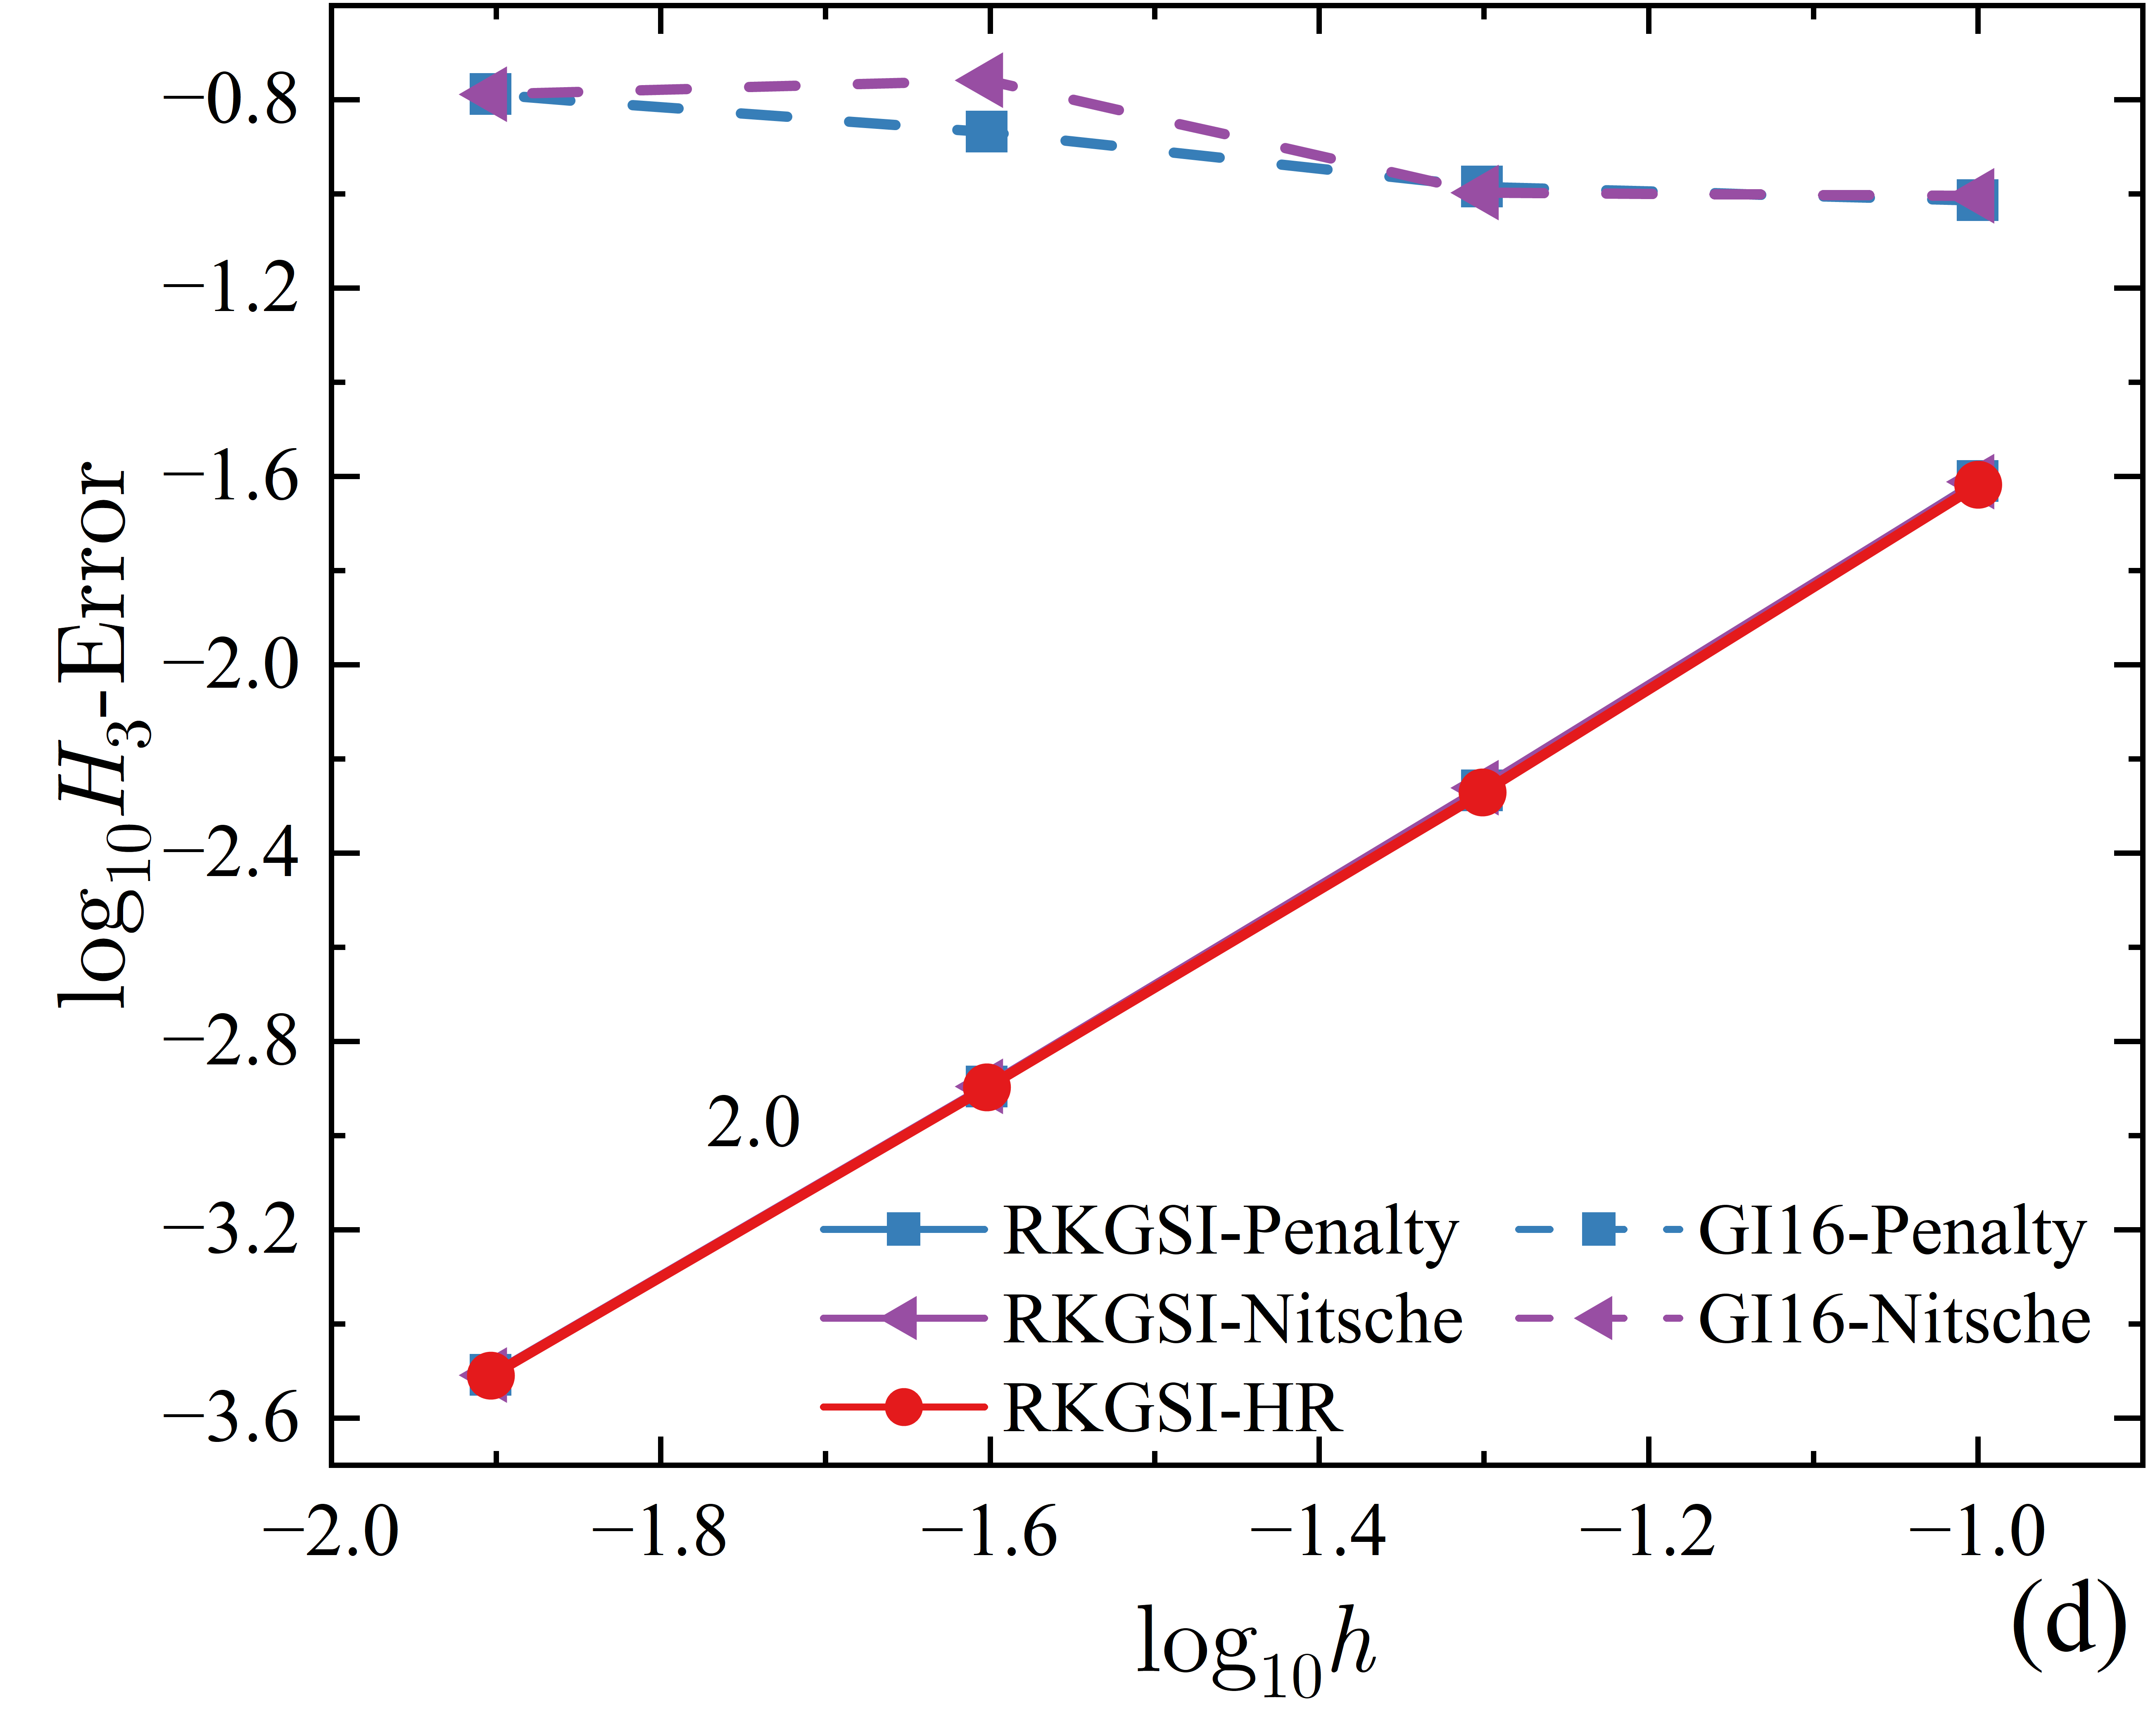
\includegraphics[width=0.49\textwidth]{figure/PHR/T/QH3.png}
    \phantomcaption\label{QH3}
    \end{subcaptiongroup}
\caption{简支等边三角形板问题四次基函数误差对比:\subref{QL2} $L_2$误差;\subref{QH1} $H_1$;误差\subref{QH2};$H_2$误差;\subref{QH3} $H_3$误差}
\label{TQLH}
\end{figure}
\begin{figure}[H]
    \centering
    \begin{subcaptiongroup}
    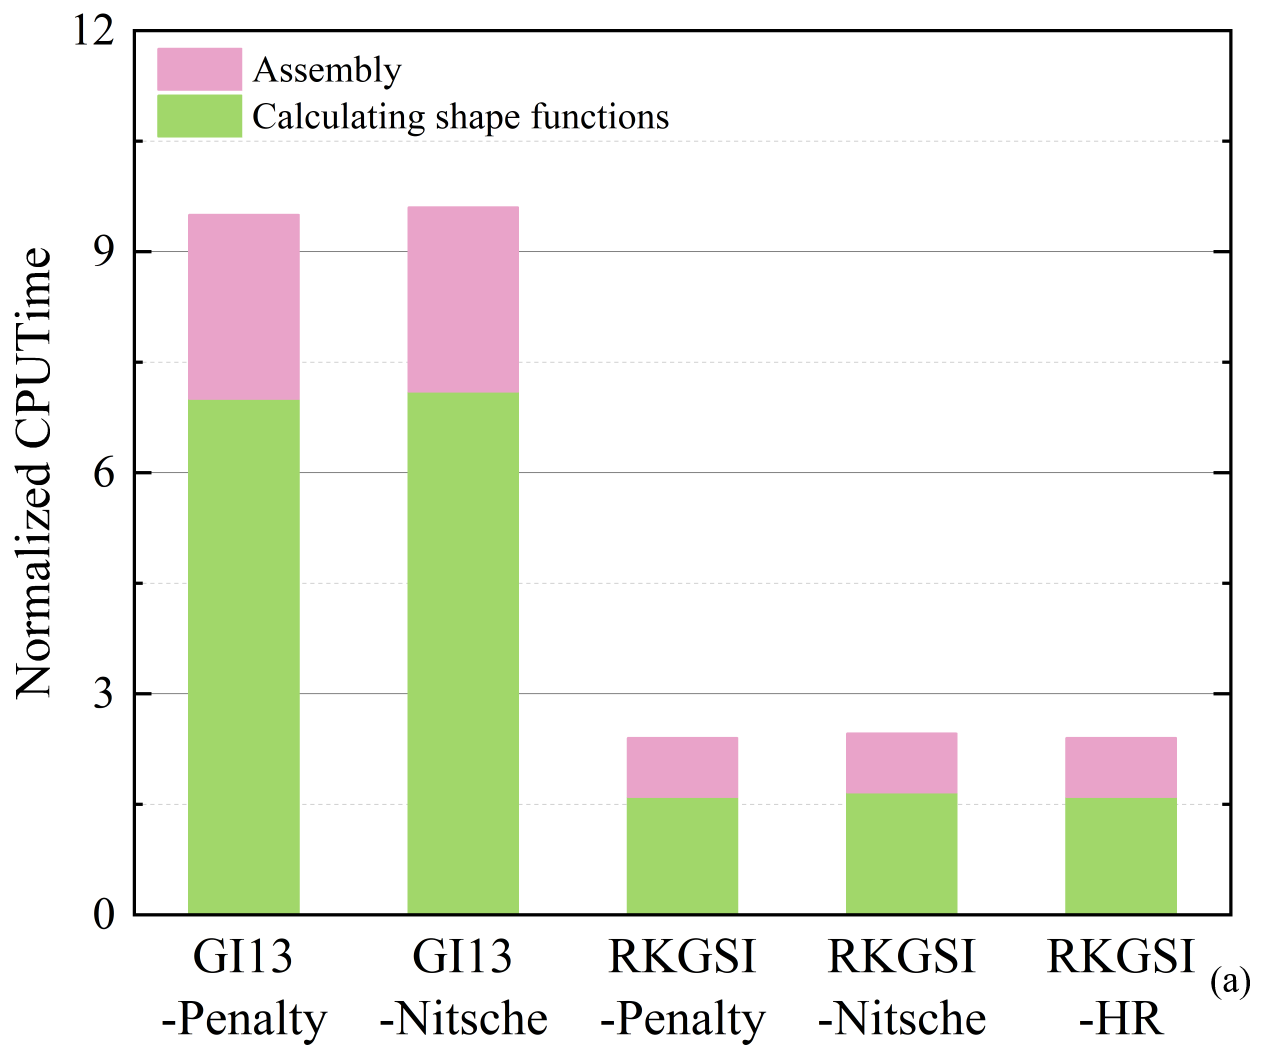
\includegraphics[width=0.49\textwidth]{figure/PHR/T/Cefficiencyomega.png}
    \phantomcaption\label{Cefficiencyomega}
    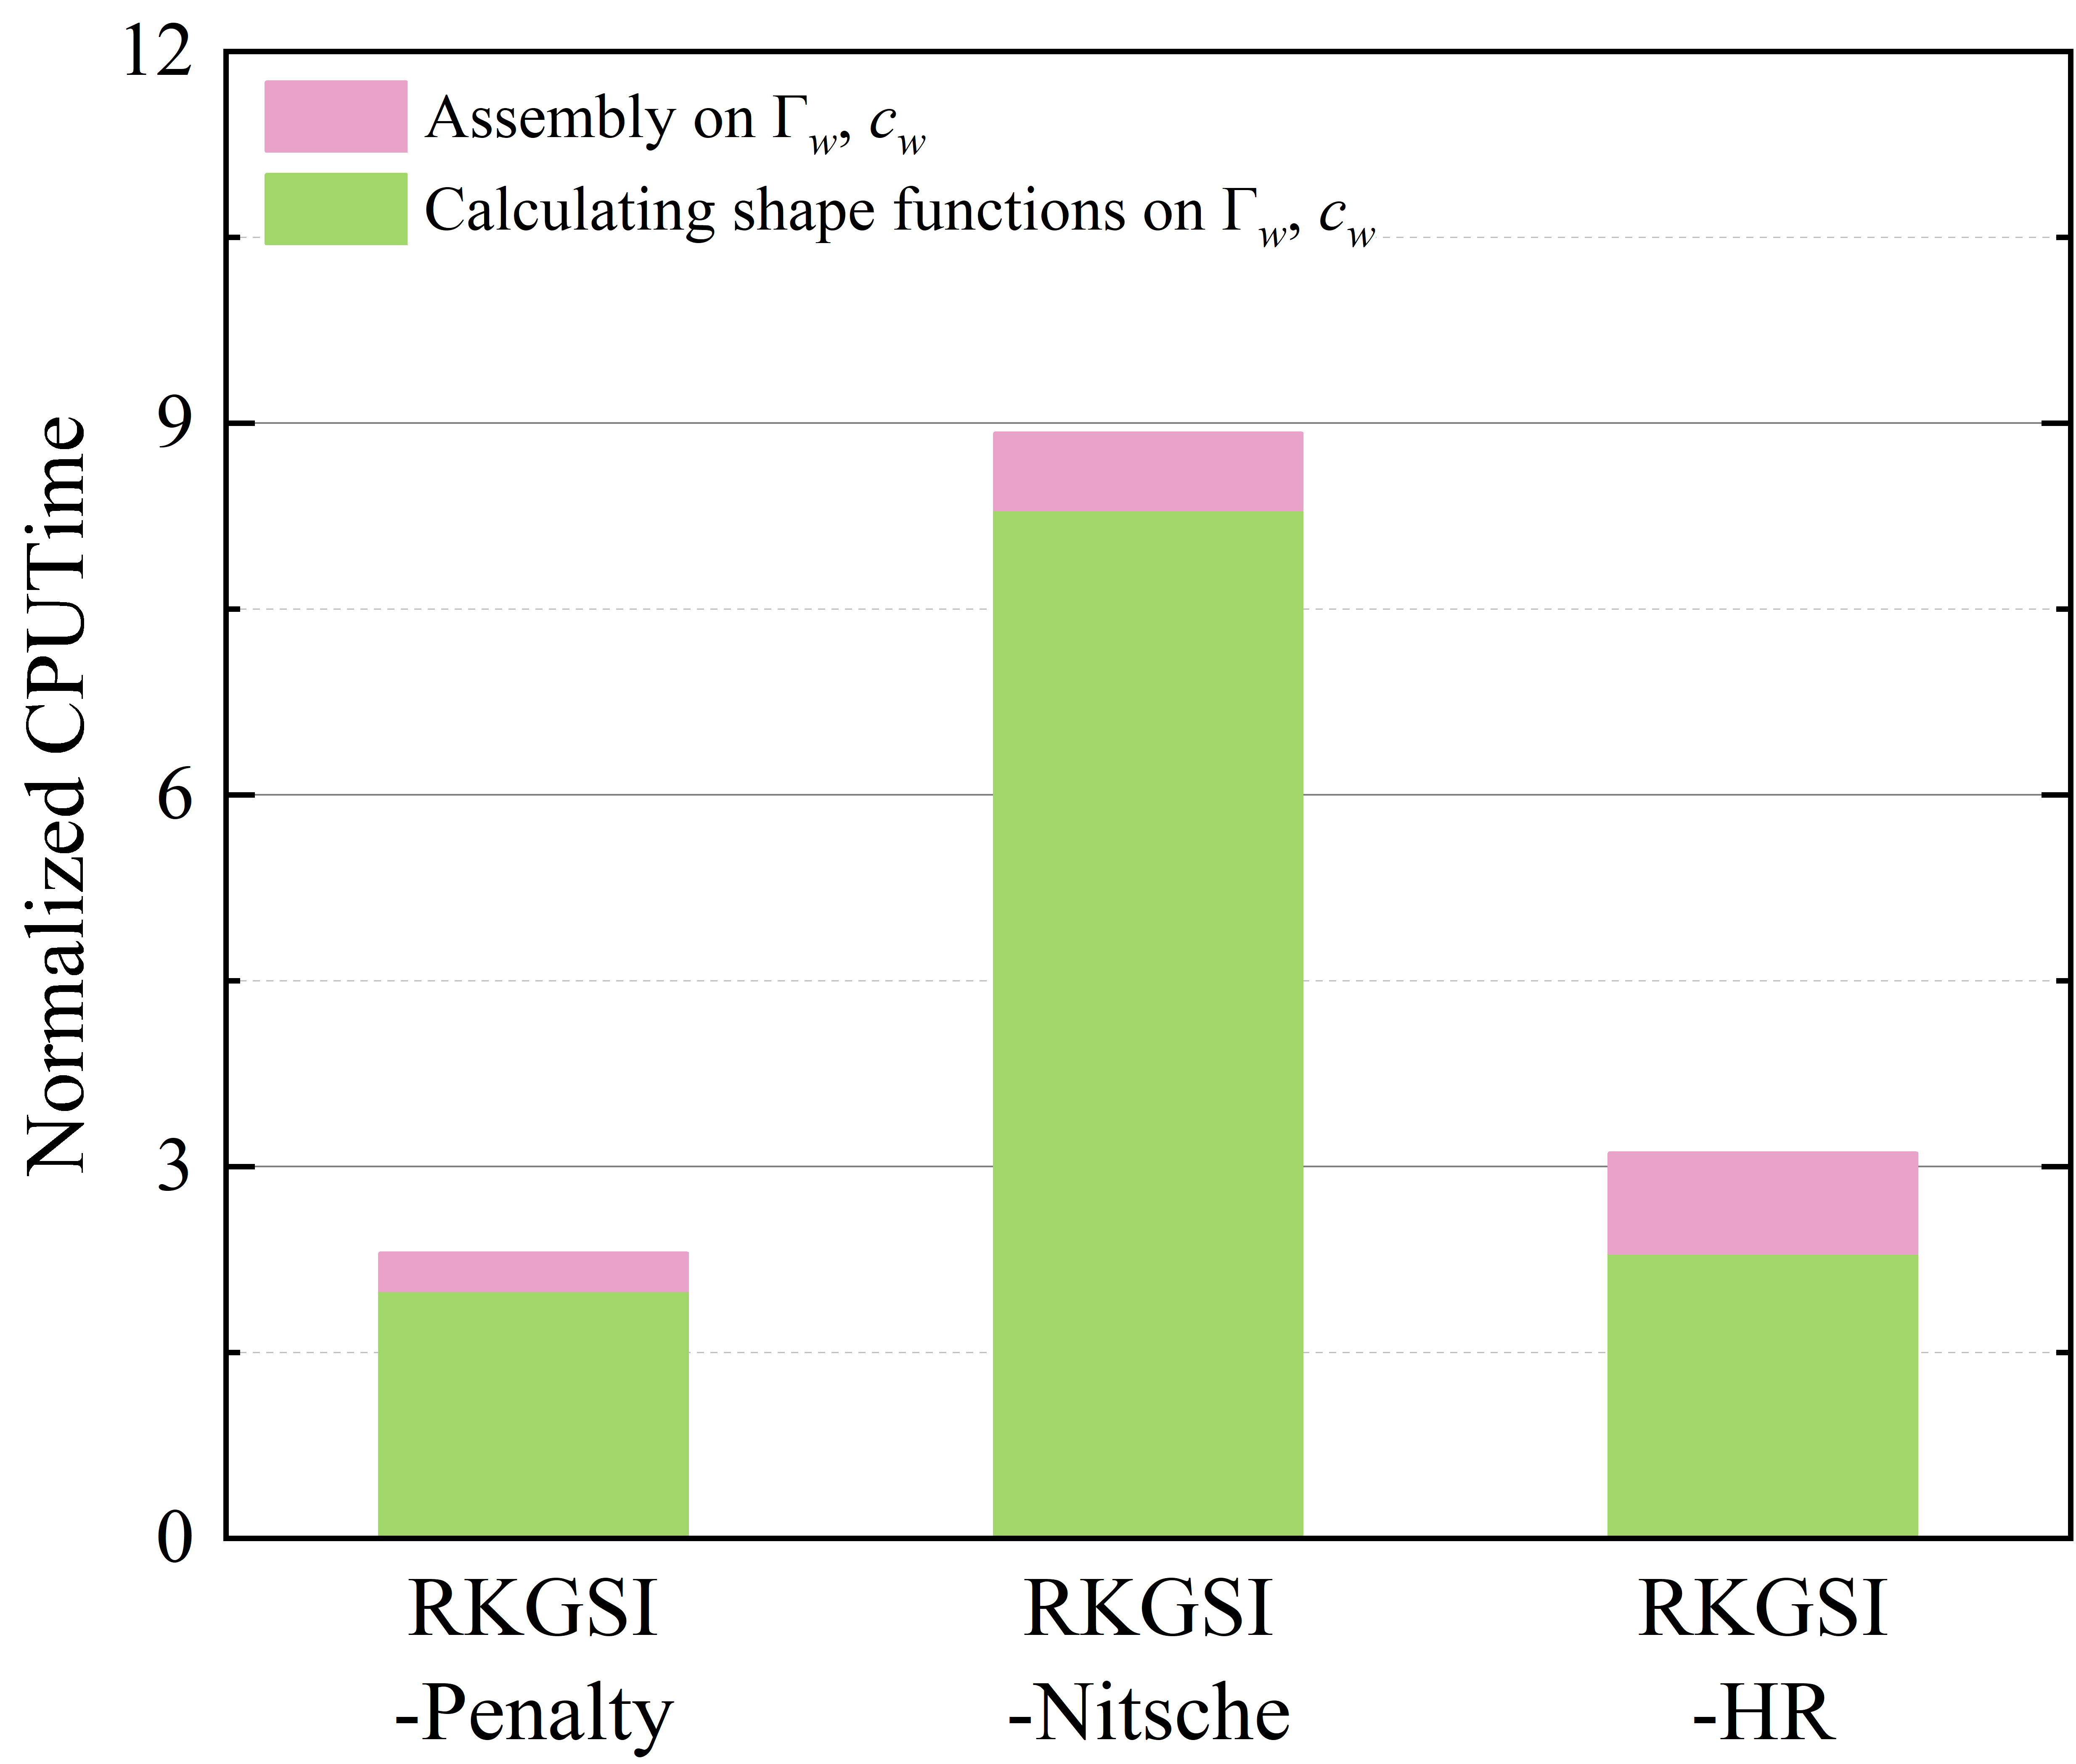
\includegraphics[width=0.49\textwidth]{figure/PHR/T/Cefficiencygamma.png}
    \phantomcaption\label{Cefficiencygamma}
    \end{subcaptiongroup}
\caption{简支等边三角形问题效率对比:\subref{Cefficiencyomega}薄板中面$\Omega$;\subref{Cefficiencygamma}本质边界条件$\Gamma_w,c_w$}
\label{Tefficiency}
\end{figure}
\newpage
\begin{figure}[H]
\centering
    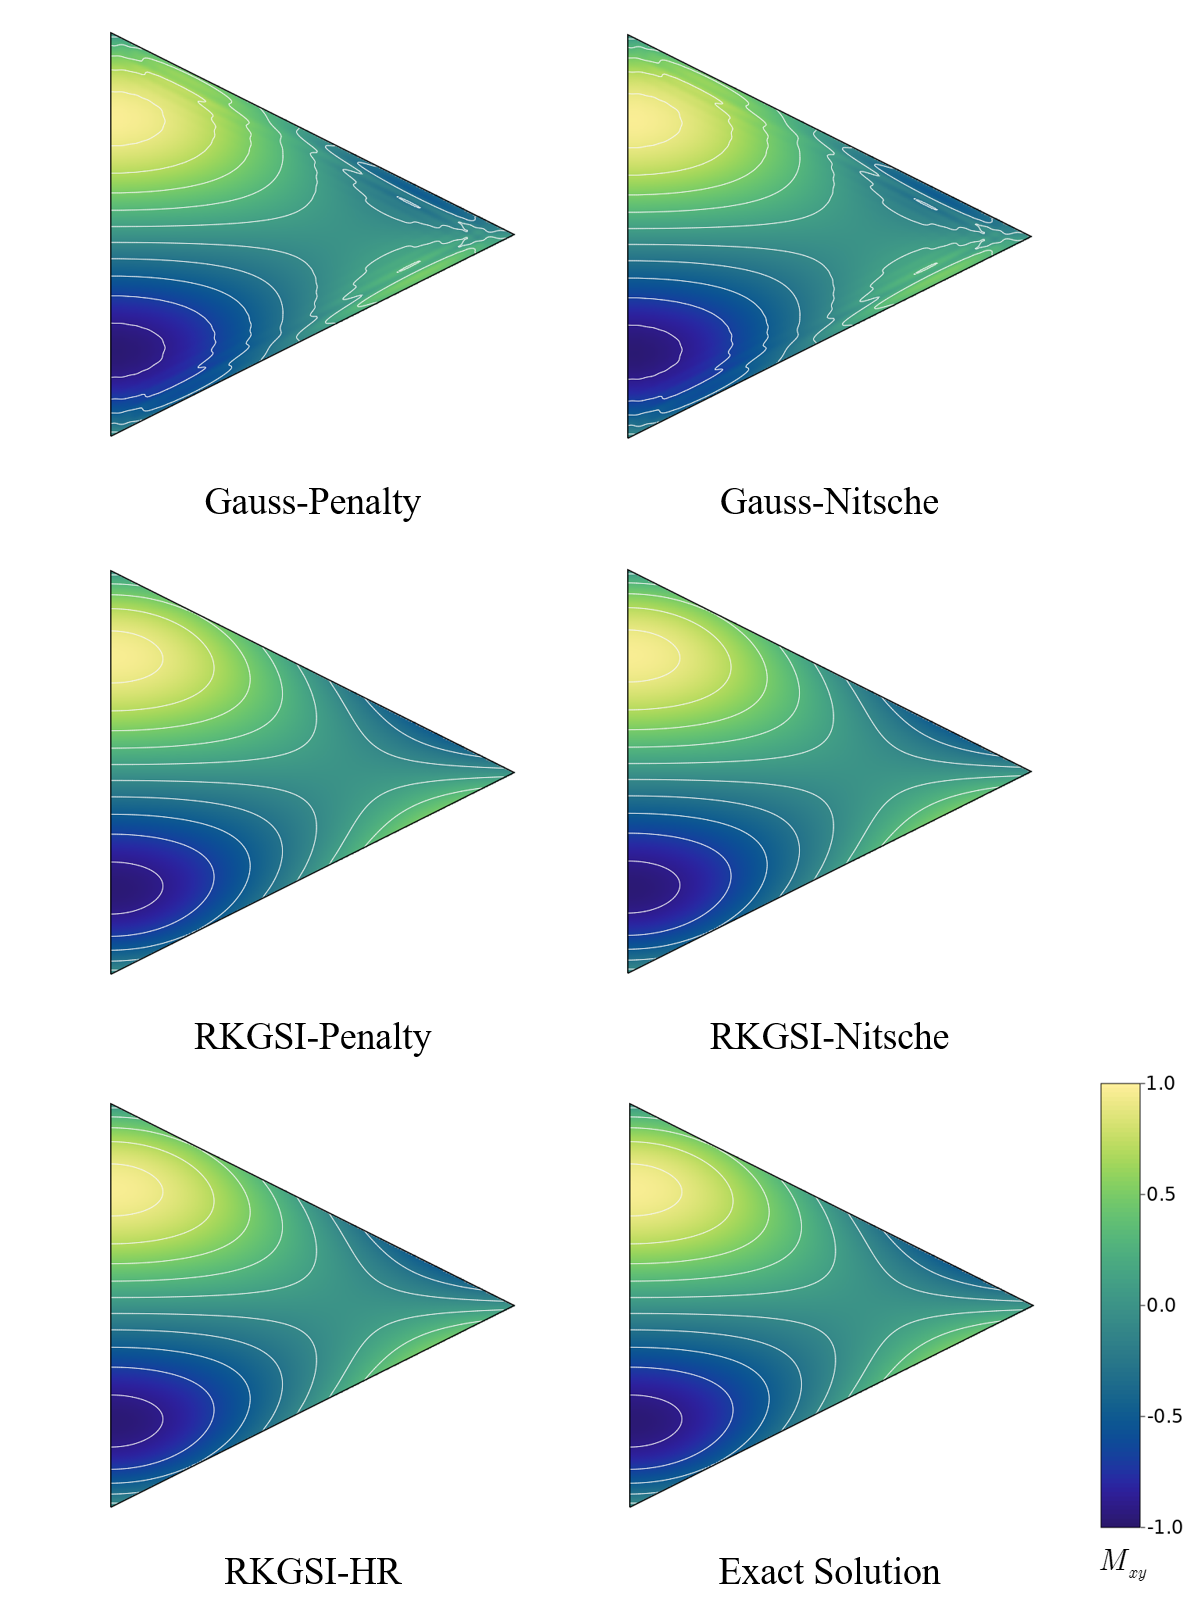
\includegraphics[scale=0.5]{figure/PHR/T/Mxy.png}
\caption{简支等边三角形板问题弯矩云图$\sigma_{xx}$应力云图}
\label{TMxy}
\end{figure}  
\subsection{简支环行板问题}
一简支环行板如图(\ref{annular})所示,其中内外径分别为$a=2$、$b=1$。在环行板的内外径边缘处分别施加弯矩$m_i=2$、$m_0=1$,
材料系数分别为抗弯刚度$\bar{D}=1$、泊松比为$\nu=0.3$。该简支环行板的精确解为:
\begin{equation}
\begin{split}
    w=\frac{(m_i-m_0)a^2b^2}{\bar D(1-\nu)(a^2-b^2)}ln\frac{r}{a}+\frac{m_ib^2-m_oa^2}{2\bar D(1+\nu)(a^2-b^2)}(r^2-a^2)
\end{split}
\end{equation}
其中:$r=\sqrt{x^2+y^2}$是点($x,y$)的极径。
\begin{figure}[H]
    \centering
    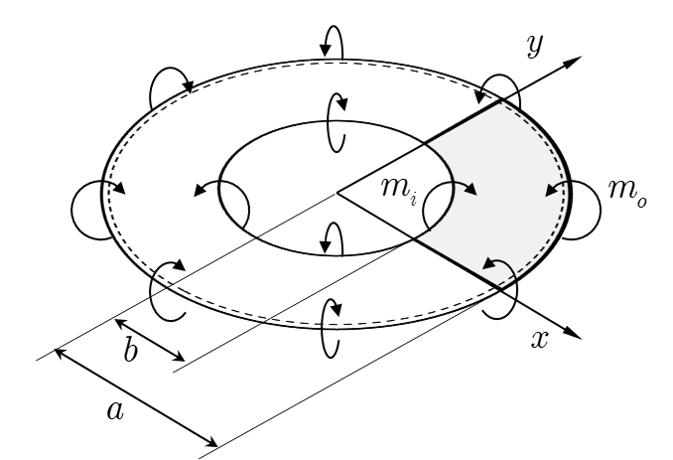
\includegraphics[scale=0.7]{figure/PHR/A/annular.png}
    \caption{简支环形板问题模型}\label{annular}
\end{figure}
如图(\ref{annularmsh})所示,简支环形问题求解域通过采用均布的153、561、2145和8385四个疏密不同的节点进行离散,
该简支环行板采用四次基函数,取相对影响域为4.5进行数值分析。\par
\begin{figure}[H]
    \centering
    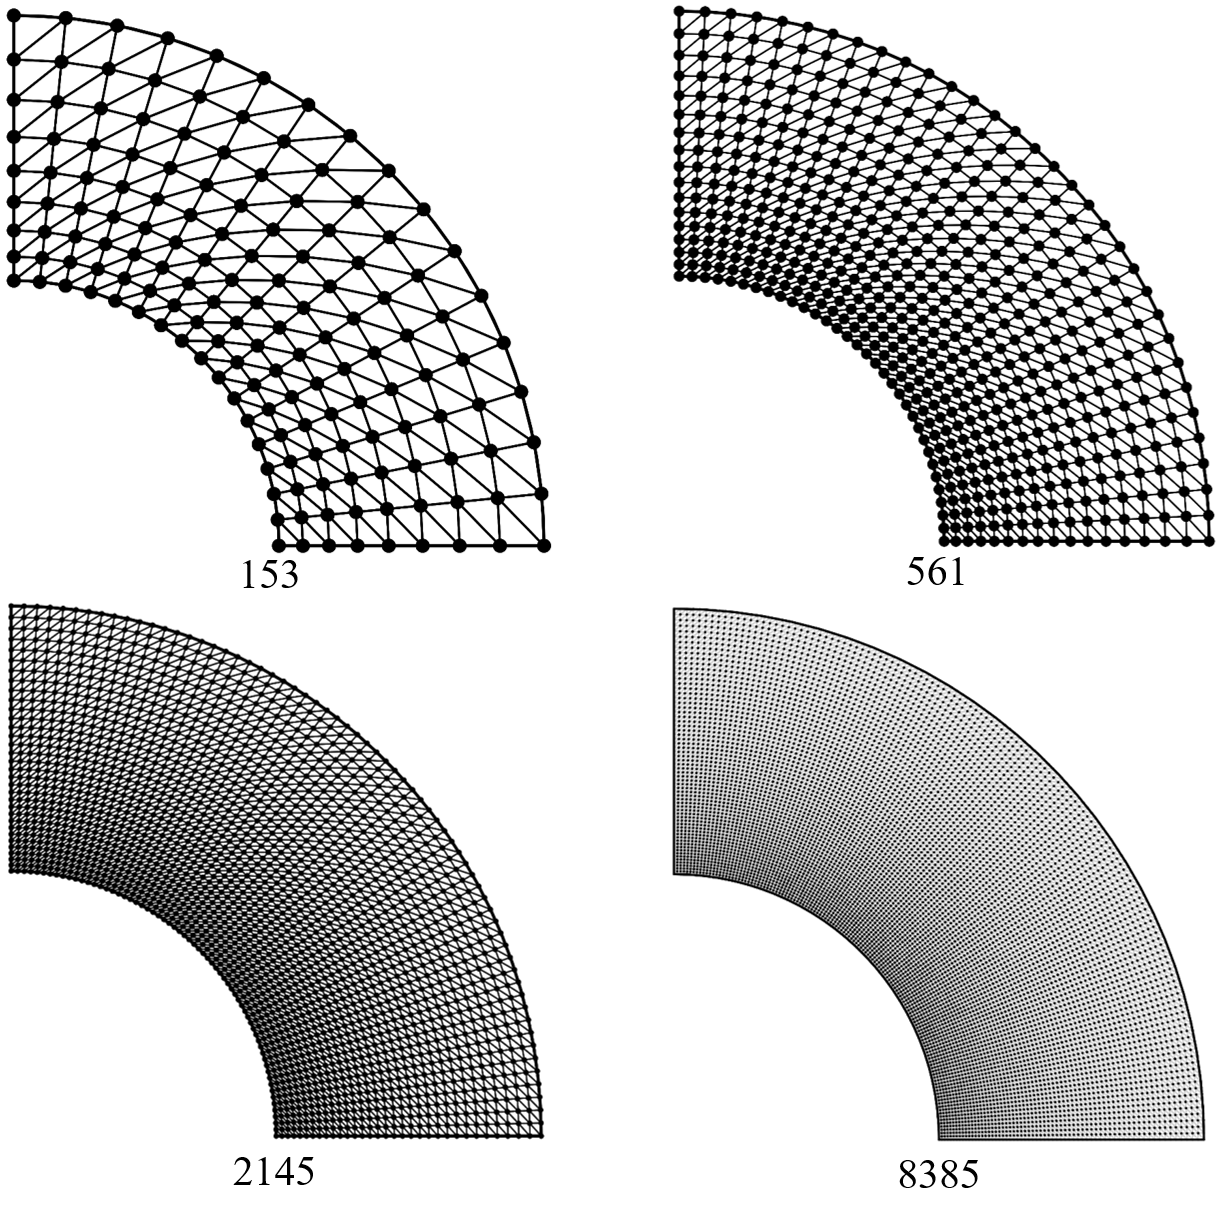
\includegraphics[scale=0.4]{figure/PHR/A/annularmsh.png}
    \caption{简支环形板问题节点离散}\label{annularmsh}
\end{figure}
图(\ref{AQLH})为简支环行板问题的位移误差和能量误差对比图,从图中可以看出“RKGSI-HR”和“RKGSI-Nitsche”同样可以达到理论误差收敛率。
图(\ref{AQcputime})为简支环行板问题在计算时间节点数和施加不同本质边界条件上的效率对比,从图中可以看出采用“RKGSI”时的效率明显高于“GI”法,
与同样满足变分一致性的“RKGSI-Nitsche”法相比,“RKGSI-HR”法在施加过程中效率明显更高。
同样根据简支环行板的弯矩云图(\ref{AMxy})也可以更进一步说明在解决薄板问题上,基于Hellinger-Reissner变分原理的本质边界条件施加方法拥有着更高的计算精度。
在简支环行板问题中,存在两个人工参数影响计算精度。从图(\ref{Aalpha})中可以看出,随着节点数的变化“RKGSI-Nitsche”法和“RKGSI-Penalty”法在达到最优精度时的人工参数值也在发生变化。
而“RKGSI-HR”法中不涉及人工参数,因此随着节点数的增加,计算精度不会受到人工参数的影响,从而提高了一种更稳定和高效的计算方法。
\begin{figure}[H]
    \centering
    \begin{subcaptiongroup}
    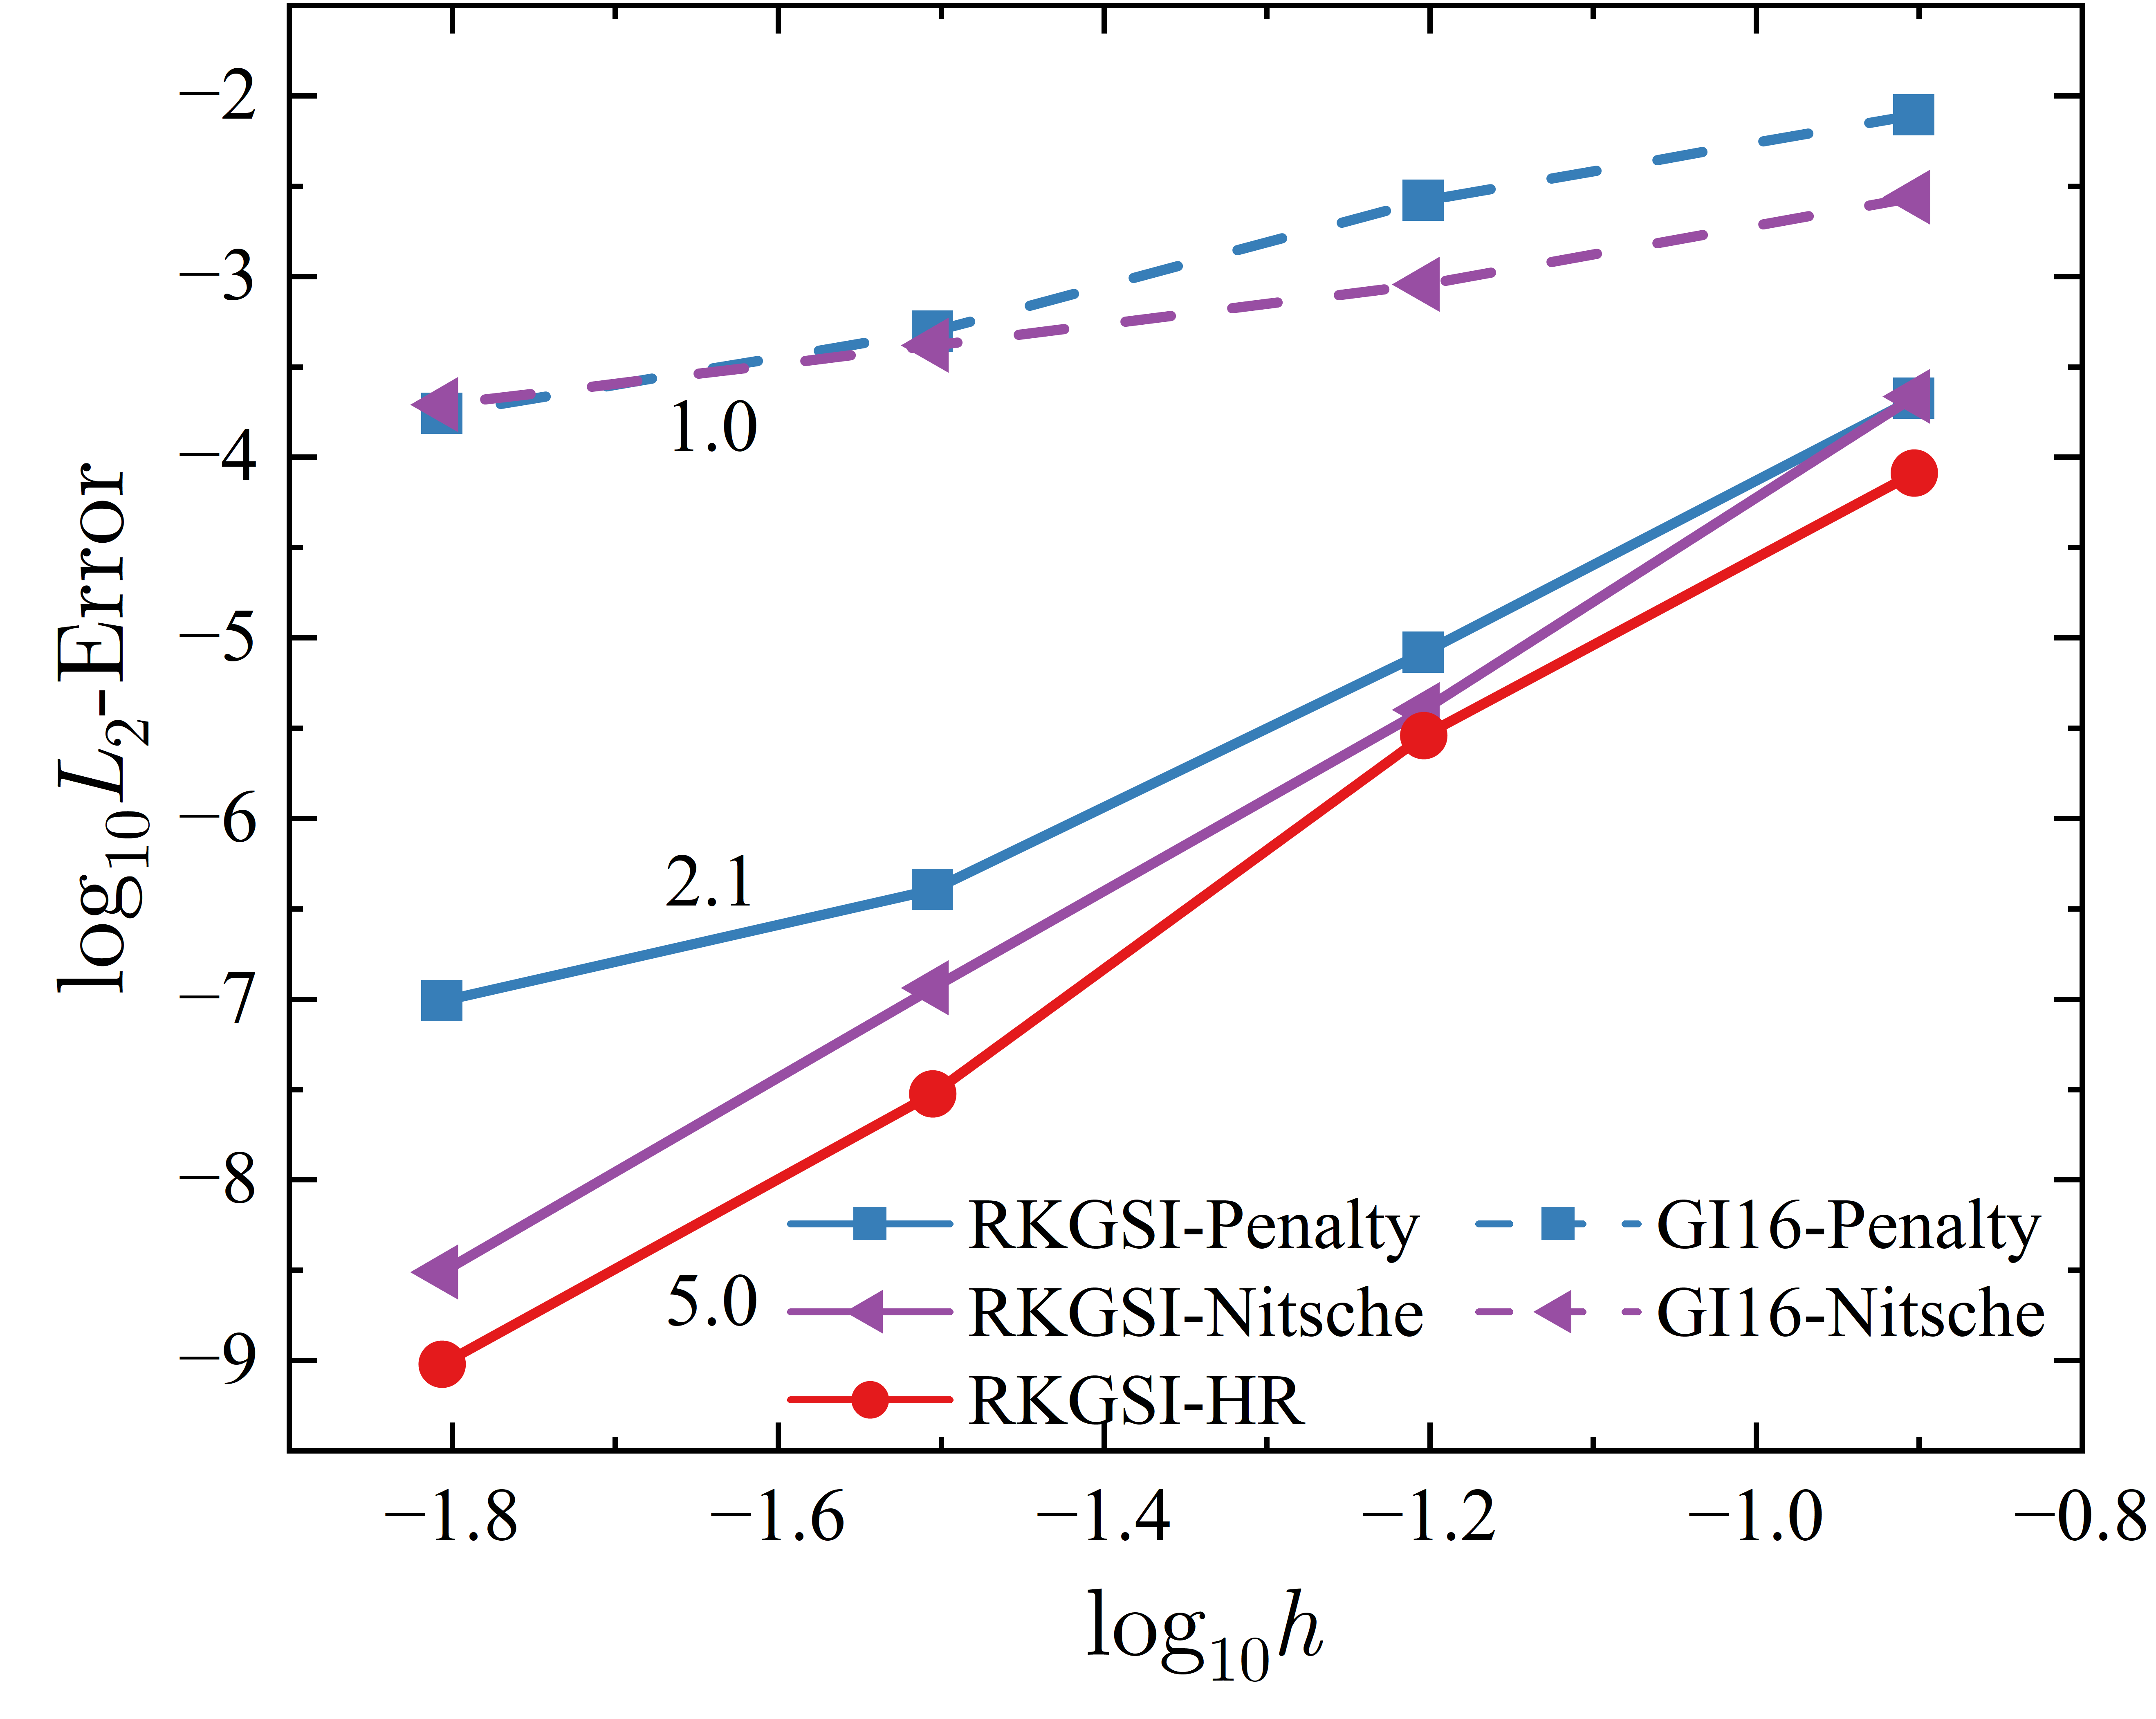
\includegraphics[width=0.49\textwidth]{figure/PHR/A/QL2.png}
    \phantomcaption\label{QL2}
    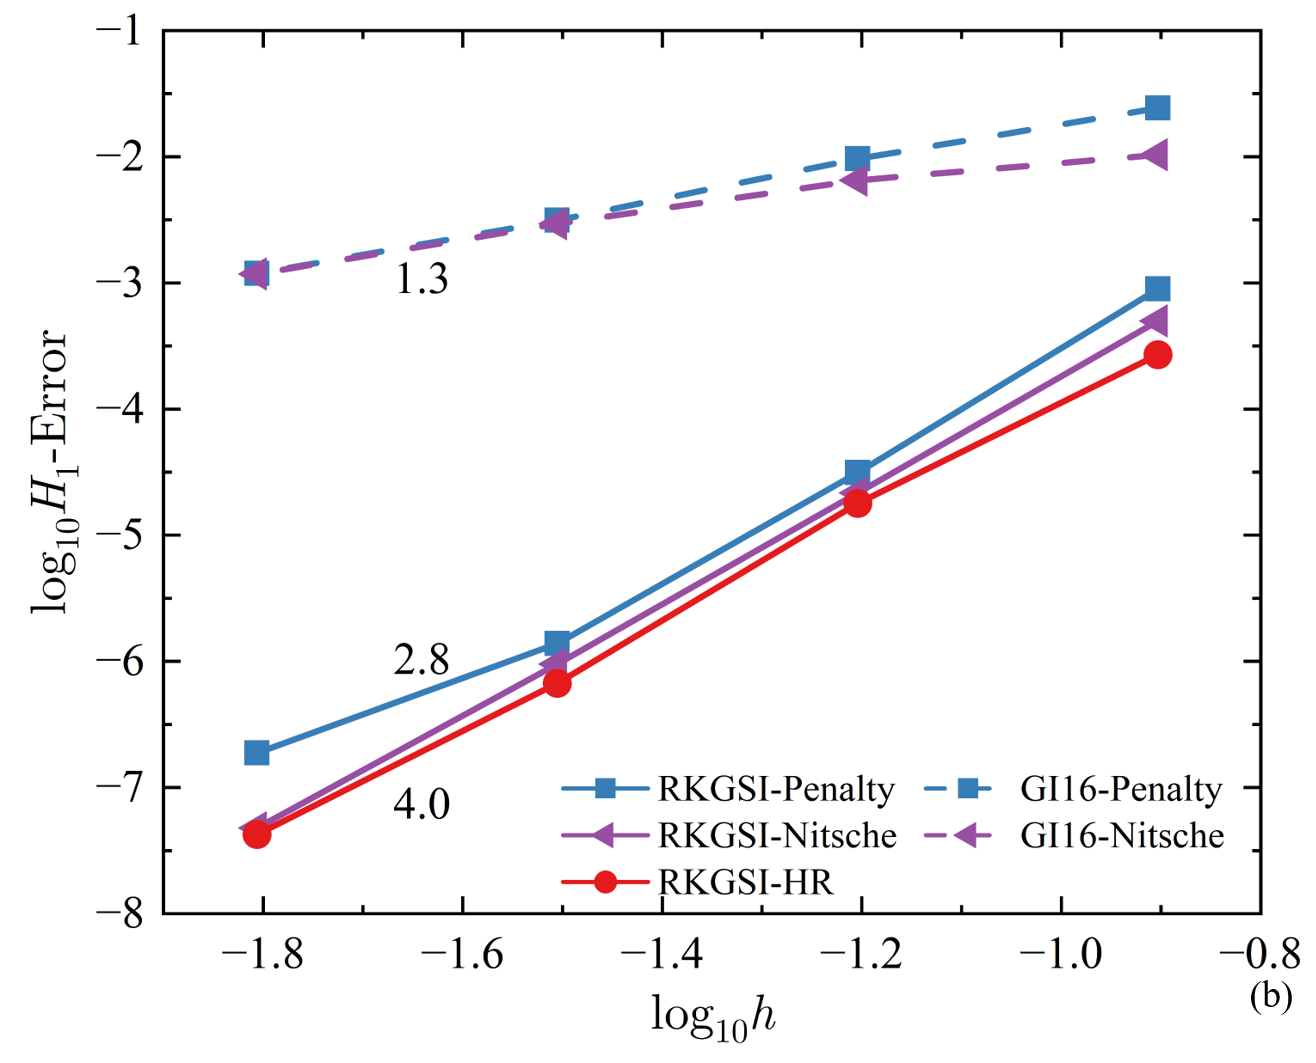
\includegraphics[width=0.49\textwidth]{figure/PHR/A/QH1.png}
    \phantomcaption\label{QH1}
    \end{subcaptiongroup}
    \begin{subcaptiongroup}
    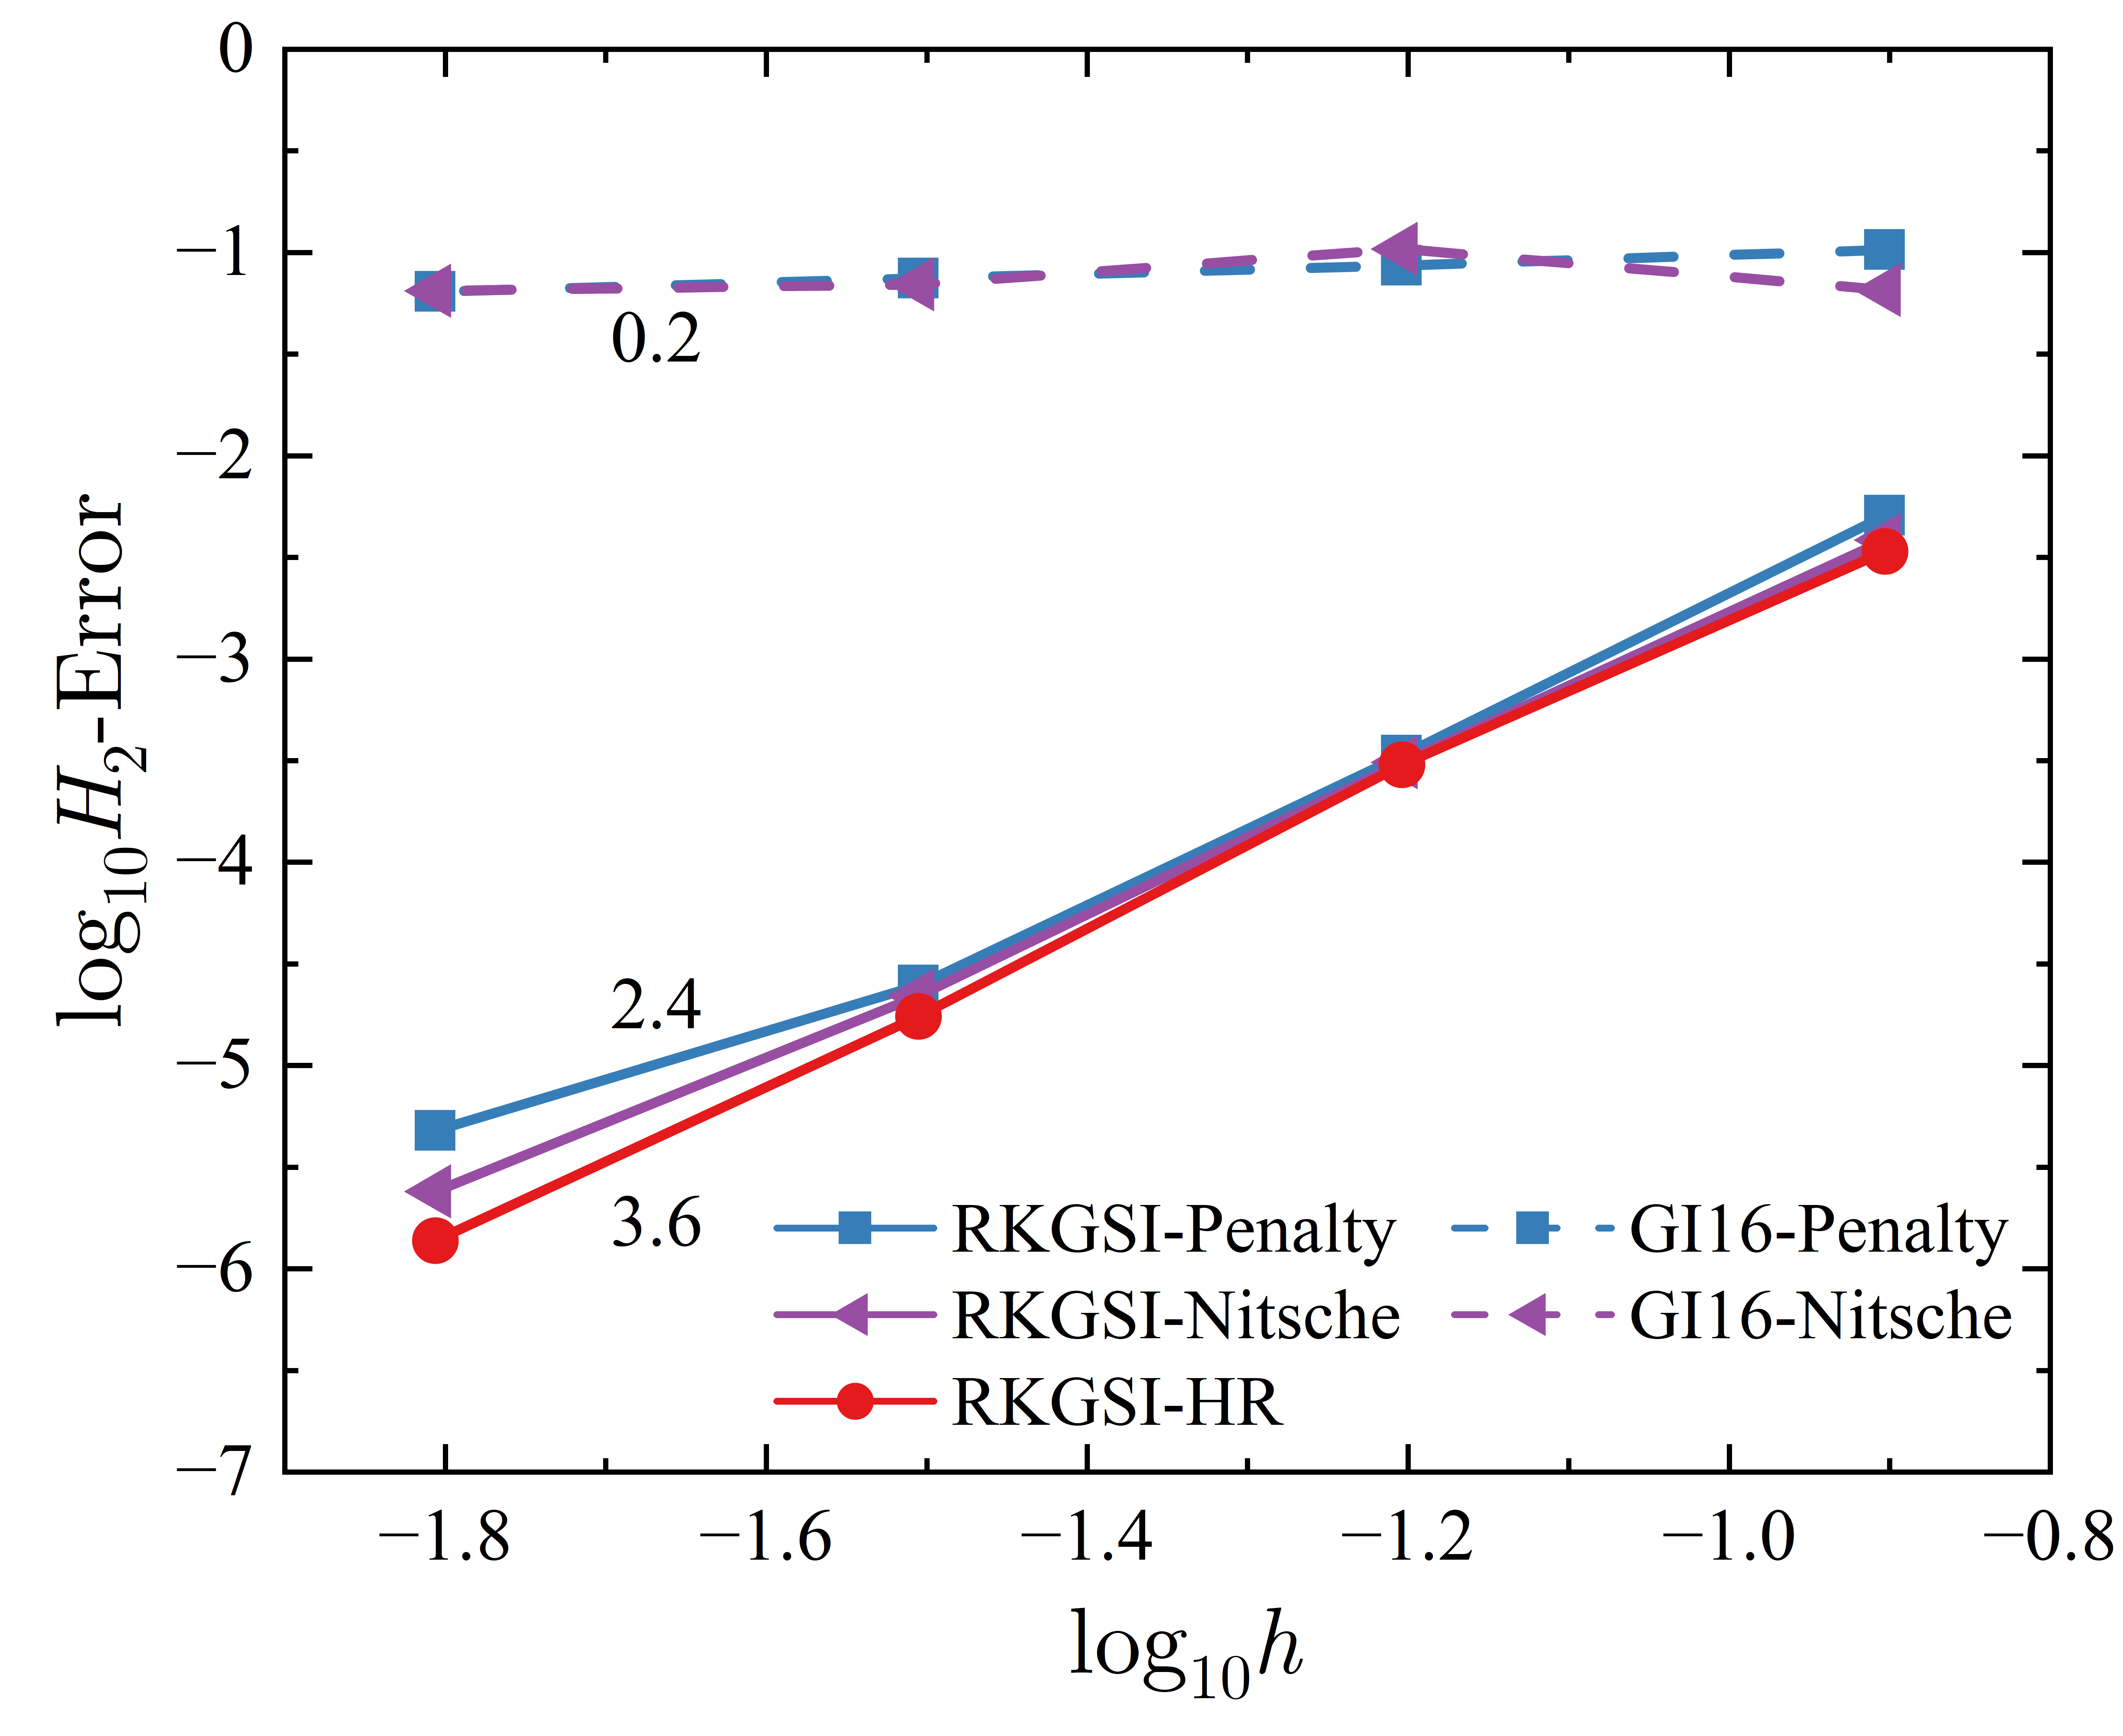
\includegraphics[width=0.49\textwidth]{figure/PHR/A/QH2.png}
    \phantomcaption\label{QH2}
    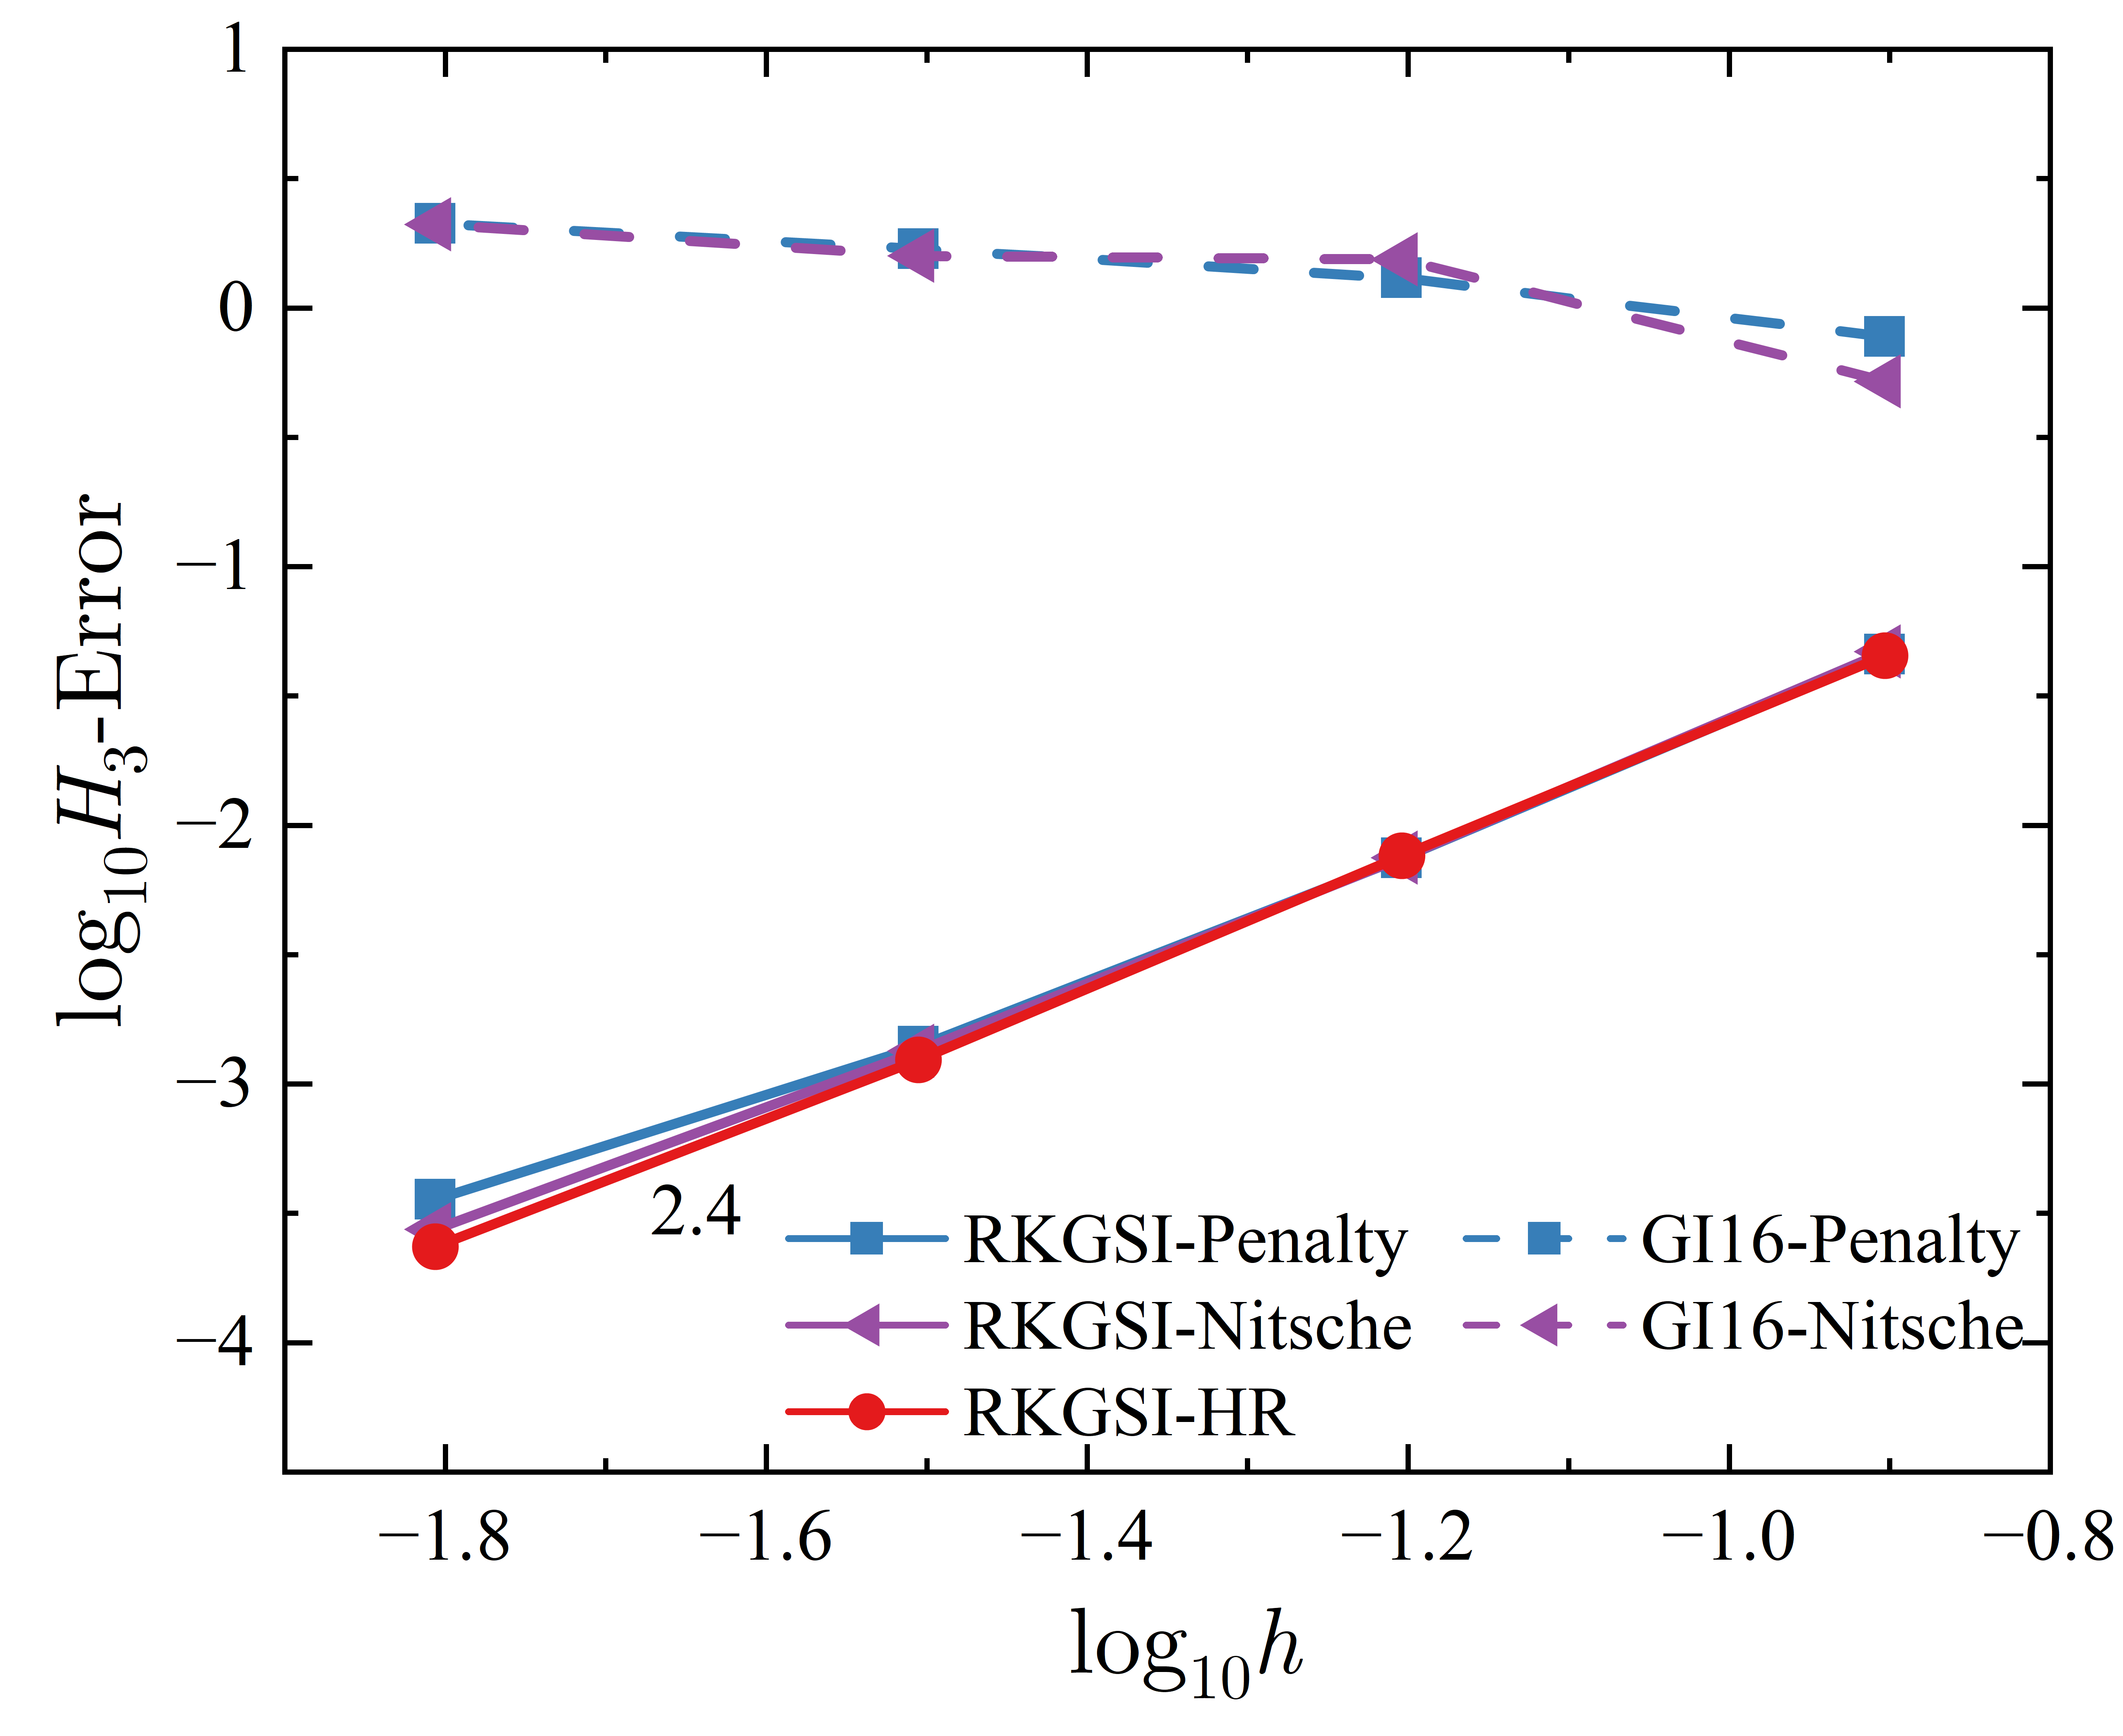
\includegraphics[width=0.49\textwidth]{figure/PHR/A/QH3.png}
    \phantomcaption\label{QH3}
    \end{subcaptiongroup}
\caption{简支环行板问题四次基函数误差对比:\subref{QL2} $L_2$误差;\subref{QH1} $H_1$;误差\subref{QH2};$H_2$误差;\subref{QH3} $H_3$误差}
\label{AQLH}
\end{figure}
\begin{figure}[H]
    \centering
    \begin{subcaptiongroup}
    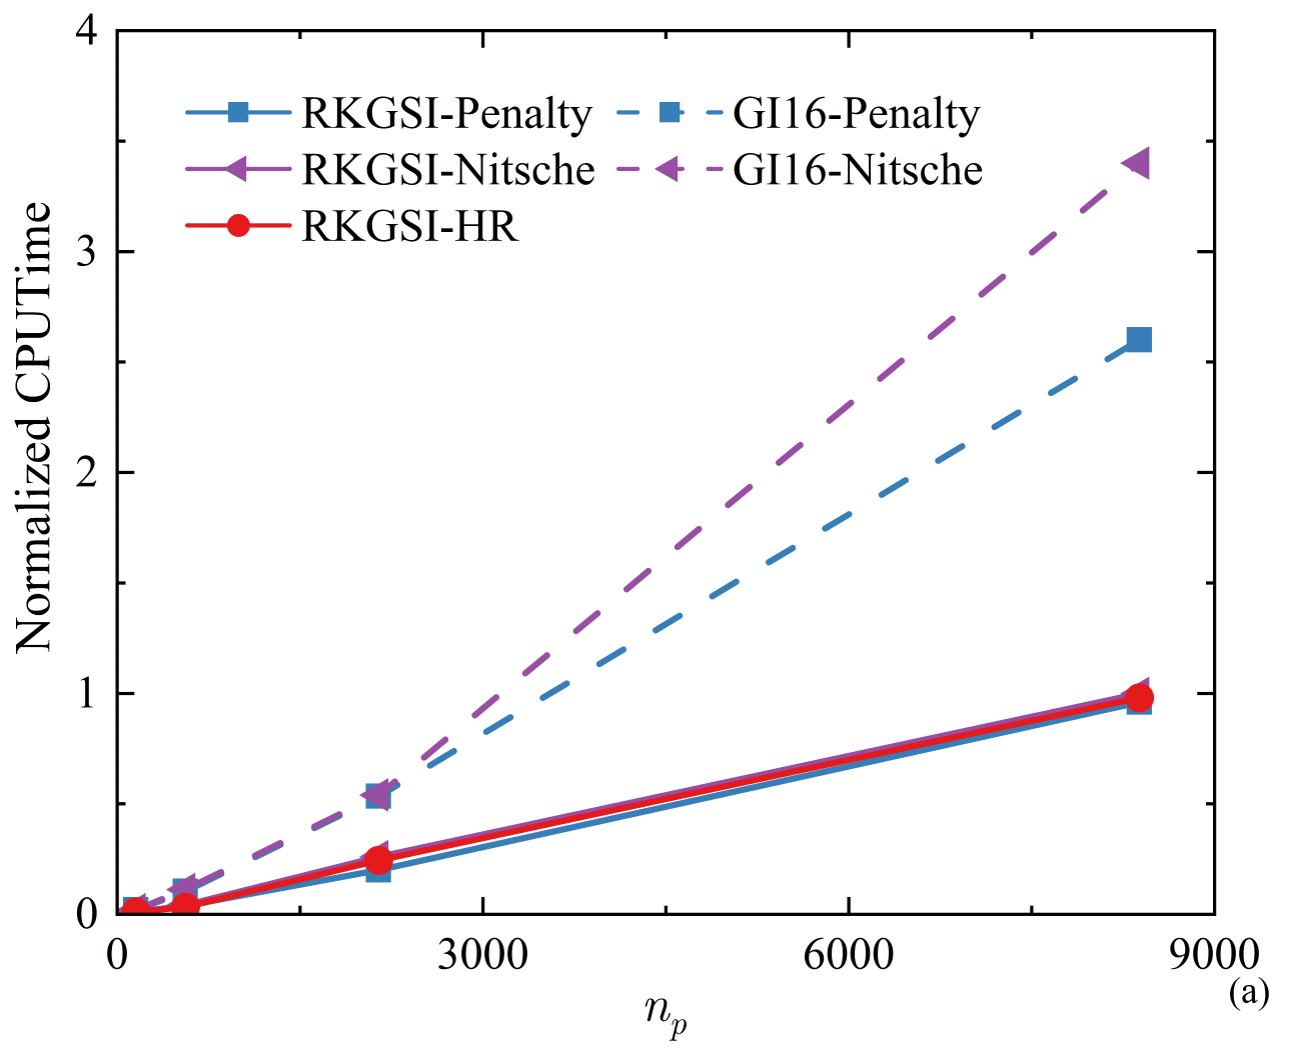
\includegraphics[width=0.49\textwidth]{figure/PHR/A/Qcputime.png}
    \phantomcaption\label{Qcputime}
    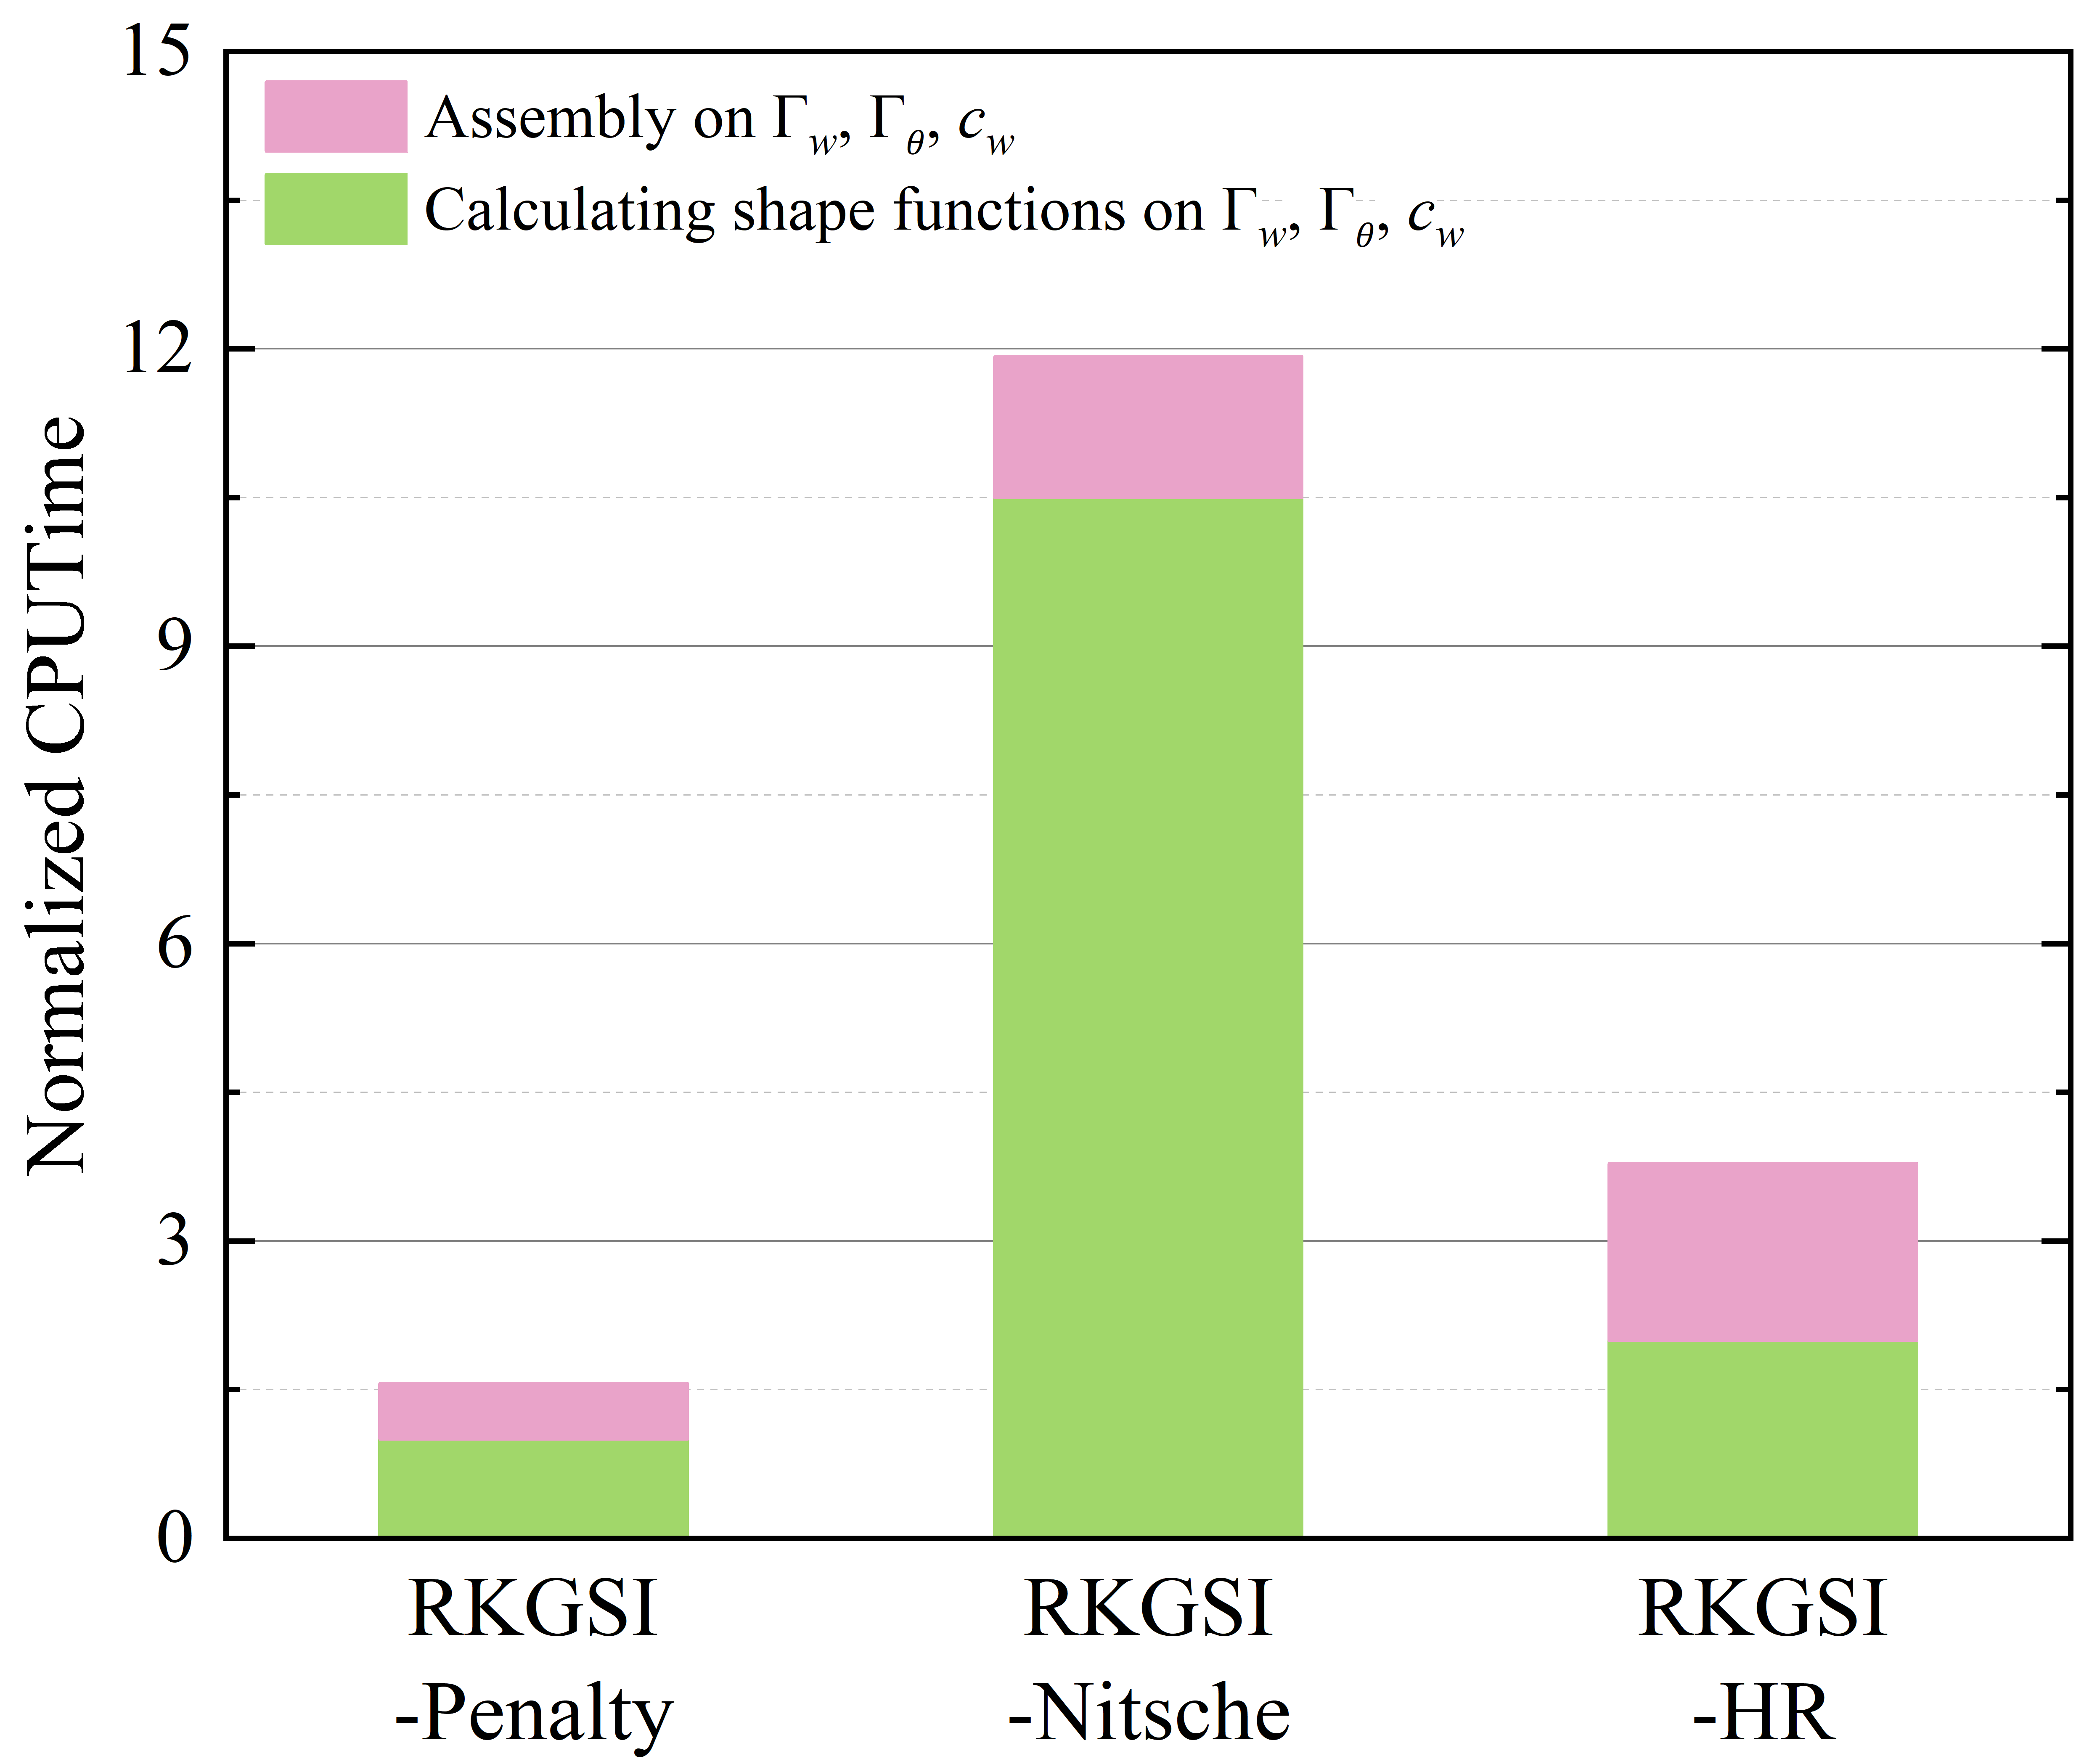
\includegraphics[width=0.49\textwidth]{figure/PHR/A/Qefficiency.png}
    \phantomcaption\label{Qefficiency}
    \end{subcaptiongroup}
\caption{简支环形板问题四次基函数效率对比:\subref{Qcputime}计算时间与节点数的关系;\subref{Cefficiency}本质边界条件施加效率分析}
\label{AQcputime}
\end{figure}
\begin{figure}[H]
    \centering
    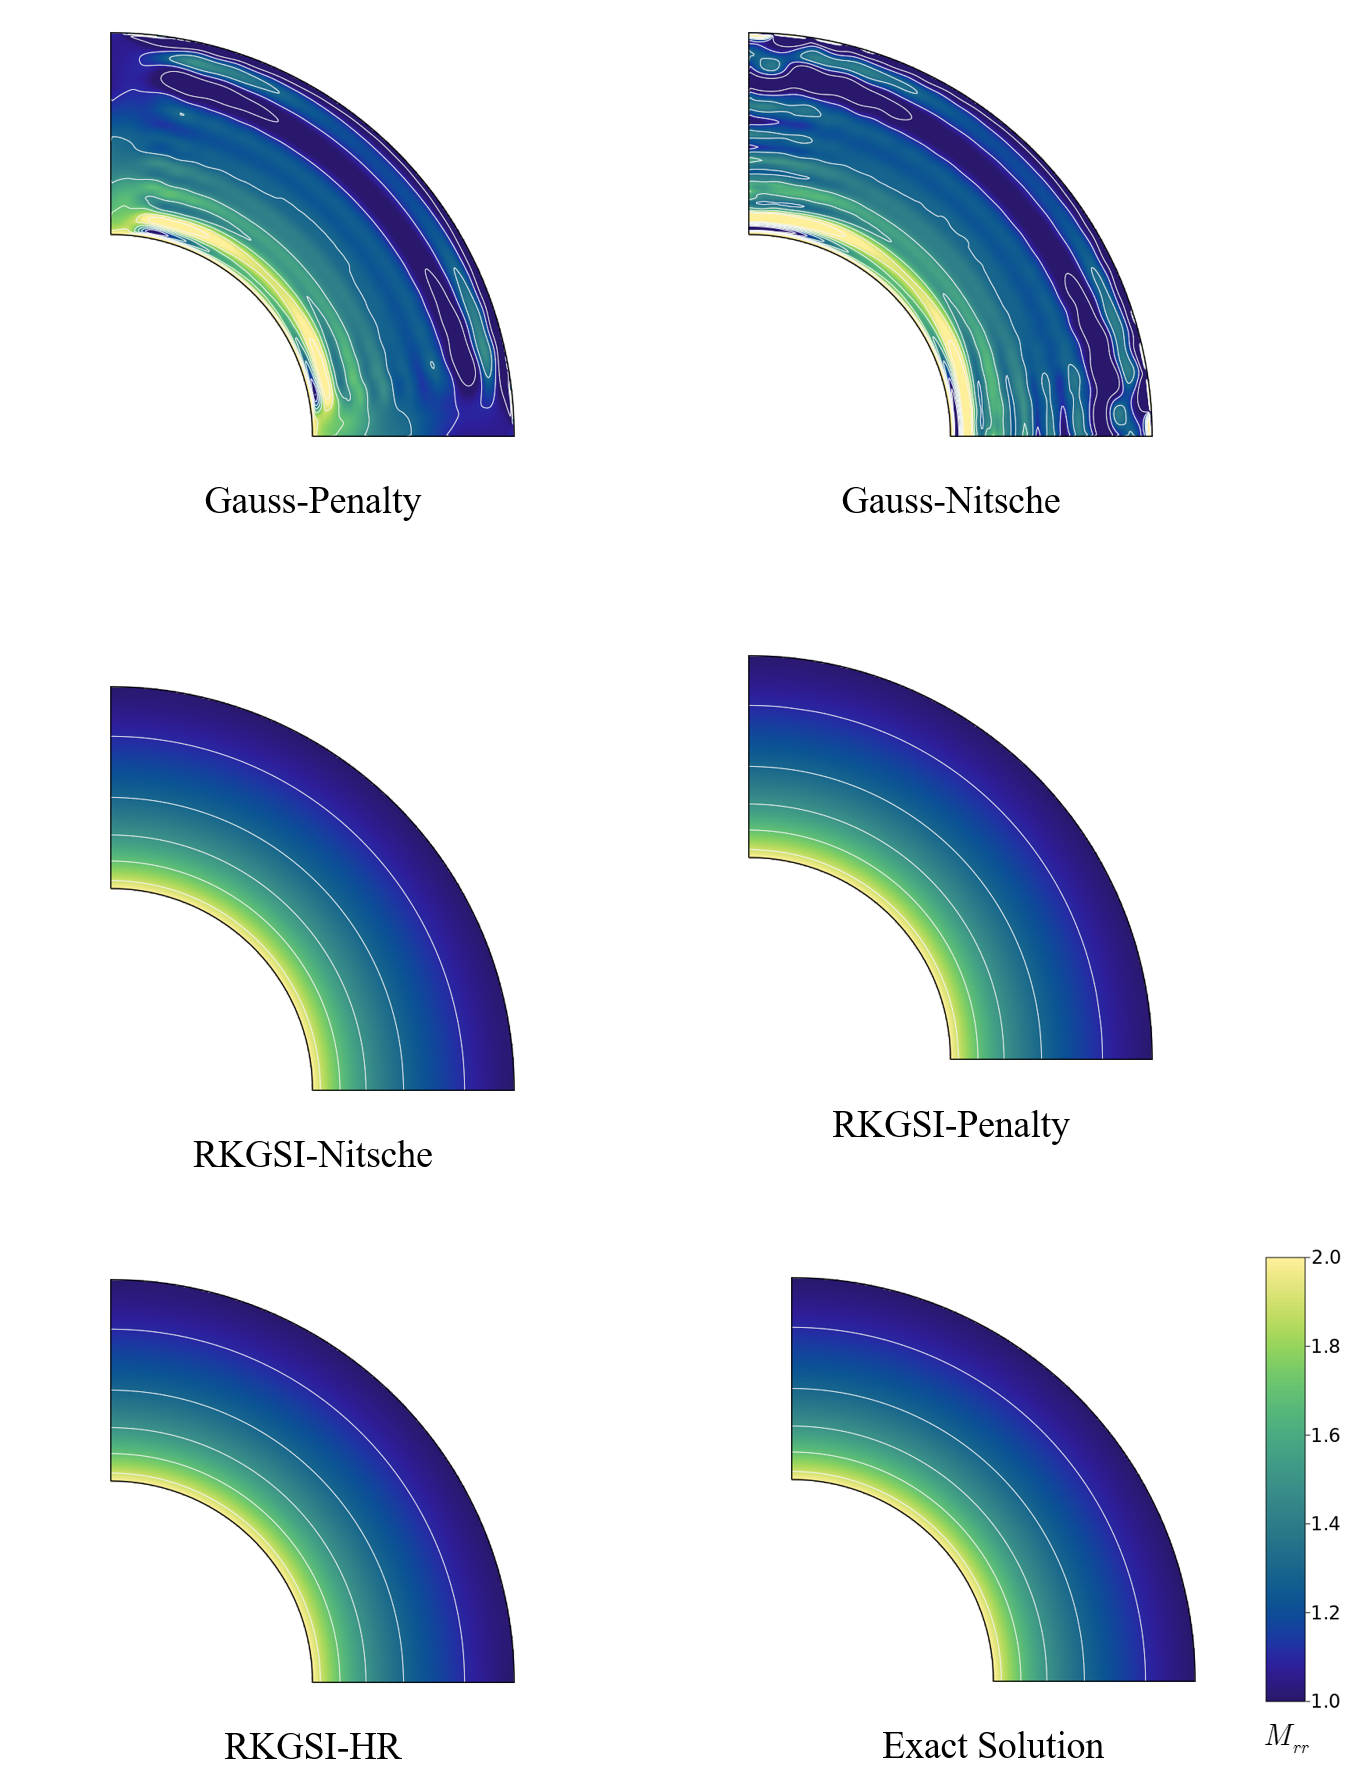
\includegraphics[scale=0.5]{figure/PHR/A/Mxy.png}
    \caption{简支环形板问题弯矩云图}\label{AMxy}
\end{figure}
\begin{figure}[H]
    \centering
    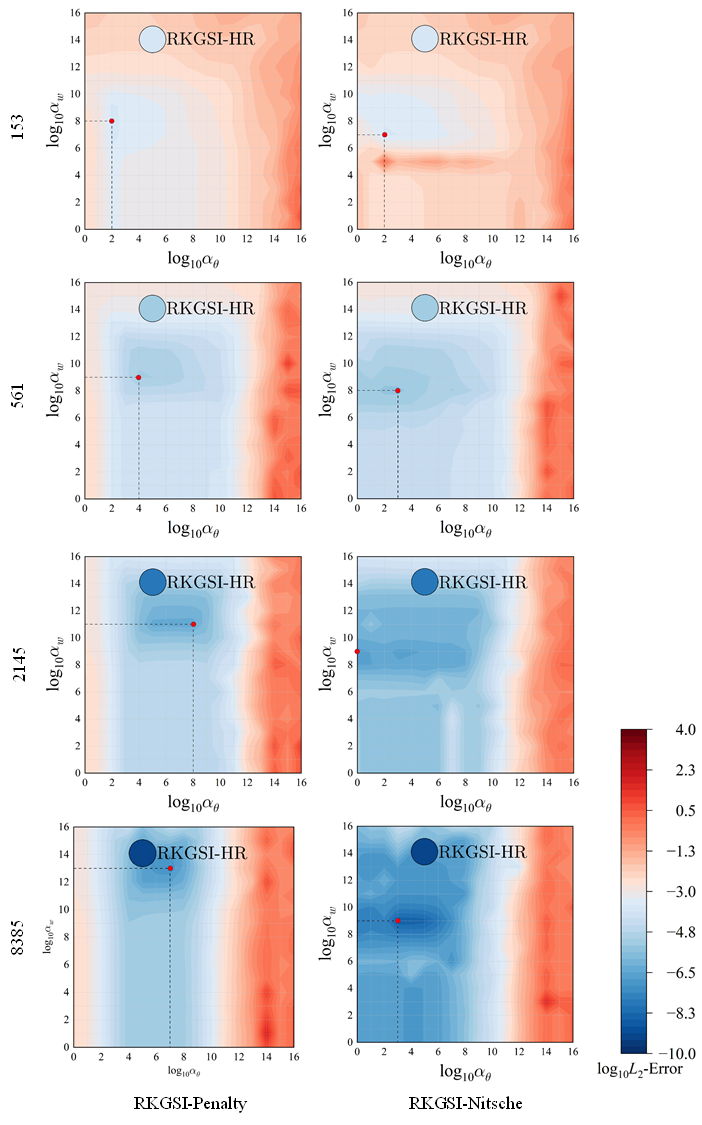
\includegraphics[scale=0.5]{figure/PHR/A/alpha.png}
    \caption{简支环形板问题人工参数敏感性分析}\label{Aalpha}
\end{figure}
\section{小结}
本章进一步介绍了基于Hellinger-Reissner变分原理的变分一致性本质边界条件施加方法,用于求解四阶薄板问题。
该方法通过采用混合离散近似Hellinger-Reissner变分原理弱形式中的挠度和弯矩,实现了满足积分约束条件用于求解高阶薄板问题的一种本质边界条件施加方法。
其中,在离散平衡控制方程中,采用传统无网格形函数对挠度进行离散,弯矩则在每个背景积分单元上以再生光滑梯度独立逼近。
通过采用再生光滑梯度积分法,该方法内嵌了局部积分约束条件,因此严格满足了每个积分单元的变分一致性。此外,由于二阶光滑梯度的计算只涉及无网格形函数及其一阶导数,有效的提高了计算效率。 
之后通过典型的数值算例进一步表明所提方法基于Hellinger-Reissner变分原理无网格薄板公式在满足变分一致性,计算精度以及计算效率方面优于采用传统高斯积分法的Nitsche法、罚函数法以及采用再生光滑梯度积分法的Nitsche法,罚函数法。
基于Hellinger-Reissner变分原理的变分一致性本质边界条件施加方法在解决薄板问题上提供了一种高效精确的边界条件施加方法。





